\documentclass[oneside,a4paper,14pt]{extreport}

% Font tiếng Việt
\usepackage[T5]{fontenc}
\usepackage[utf8]{inputenc}
\DeclareTextSymbolDefault{\DH}{T1}

% Tài liệu tham khảo
\usepackage[
    style=ieee,
	sorting=nty,
    backend=biber,
	defernumbers=true]{biblatex}
\usepackage[unicode]{hyperref} % Bookmark tiếng Việt
\addbibresource{References/references.bib}

\makeatletter
\def\blx@maxline{77}
\makeatother

% Chèn hình, các hình trong luận văn được để trong thư mục Images/
\usepackage{float}
\usepackage{graphicx}
\graphicspath{ {Images/} }

% Chèn và định dạng mã nguồn
\usepackage{listings}
\usepackage{color}
\definecolor{codegreen}{rgb}{0,0.6,0}
\definecolor{codegray}{rgb}{0.5,0.5,0.5}
\definecolor{codepurple}{rgb}{0.58,0,0.82}
\definecolor{backcolour}{rgb}{0.95,0.95,0.92}
\lstdefinestyle{mystyle}{
    backgroundcolor=\color{backcolour},   
    commentstyle=\color{codegreen},
    keywordstyle=\color{magenta},
    numberstyle=\tiny\color{codegray},
    stringstyle=\color{codepurple},
    basicstyle=\footnotesize,
    breakatwhitespace=false,         
    breaklines=true,                 
    captionpos=b,                    
    keepspaces=true,                 
    numbers=left,                    
    numbersep=5pt,                  
    showspaces=false,                
    showstringspaces=false,
    showtabs=false,                  
    tabsize=2
}
\lstset{style=mystyle}

% Chèn và định dạng mã giả
\usepackage{amsmath}
\usepackage{amssymb}
\usepackage{amsthm}
\usepackage{algorithm}
\usepackage[noend]{algpseudocode}
\makeatletter
\def\BState{\State\hskip-\ALG@thistlm}
\makeatother

\newtheorem{assumption}{Giả định}
\newtheorem{proposition}{Mệnh đề}
\newtheorem{theorem}{Định lý}
\newtheorem{lemma}{Bổ đề}
\newtheorem{definition}{Định nghĩa}

% Bảng biểu
\usepackage{tabularx}
\usepackage{multirow}
\usepackage{array}
\newcolumntype{L}[1]{>{\raggedright\let\newline\\\arraybackslash\hspace{0pt}}m{#1}}
\newcolumntype{C}[1]{>{\centering\let\newline\\\arraybackslash\hspace{0pt}}m{#1}}
\newcolumntype{R}[1]{>{\raggedleft\let\newline\\\arraybackslash\hspace{0pt}}m{#1}}
\newcolumntype{Y}{>{\centering\arraybackslash}X}

% Từ viết tắt
\usepackage[acronym,toc,nonumberlist]{glossaries}
\makeglossaries
\loadglsentries{Glossary/glossary.tex}

% Đổi tên mặc định
\renewcommand{\chaptername}{Chương}
\renewcommand{\figurename}{Hình}
\renewcommand{\tablename}{Bảng}
\renewcommand{\contentsname}{Mục lục}
\renewcommand{\listfigurename}{Danh sách hình}
\renewcommand{\listtablename}{Danh sách bảng}
\renewcommand{\appendixname}{Phụ lục}

% Định dạng chapter
\usepackage{titlesec}
\titleformat{\chapter}
    [display] 
    {\normalfont\bfseries\Large}{\chaptername \ \thechapter}{10pt}{\huge}
\titlespacing*{\chapter}{0pt}{-10pt}{40pt} %khoảng cách giữa chapter và đầu trang

\titleformat{\section}
    {\normalfont\bfseries\large}{\thesection}{1em}{}
 
\titleformat{\subsection}
    {\normalfont\bfseries\normalsize}{\thesubsection}{1em}{}
  
% Dãn dòng 1.5
\usepackage{setspace}
\onehalfspacing

% Thụt vào đầu dòng
\usepackage{indentfirst}

% Canh lề
\usepackage[
  top=20mm,
  bottom=10mm,
  left=30mm,
  right=20mm,
  footskip = 15mm,
  includefoot]{geometry}

% Quản lý pdf
\usepackage{pdfpages}

% Quản lý itemize
\usepackage{enumitem}

% Trang bìa
\usepackage{tikz}
\usetikzlibrary{calc}
\newcommand\HRule{\rule{\textwidth}{1pt}}

% ========================================================================================= %
% Ý: Thông tin chung về KLTN - sinh viên điền vào đây để tự động update các trang khác  %
% ========================================================================================= %
\newcommand{\tenSV}{Nguyễn~Lê~Tuấn~Khải}
\newcommand{\mssv}{20120503}
\newcommand{\tenKL}{Giải~thích~Negative~Transfer~trong~Meta-Learning}
\newcommand{\tenGVHD}{GS.TS~Lê~Hoài~Bắc}
\newcommand{\tenBM}{Khoa~học~máy~tính}

%%%%%%%%%%%%%%%%%%%%%%%%%%%%%%%%%%%%%%%%%%%%%%%%%%%%%%%%%%%%%%%%%%%%%%%%%%%%%%%%%%%%%%%%%%%%%
\begin{document}

\begin{titlepage}

\begin{center}
%ĐẠI HỌC QUỐC GIA THÀNH PHỐ HỒ CHÍ MINH\\
TRƯỜNG ĐẠI HỌC KHOA HỌC TỰ NHIÊN\\
\textbf{KHOA CÔNG NGHỆ THÔNG TIN}\\[2cm]


{ \Large \bfseries \tenSV\\[2cm] } 

{ \Large \bfseries  \MakeUppercase{\tenKL}\\[3cm]} 

\large KHÓA LUẬN TỐT NGHIỆP CỬ NHÂN\\
\large CHƯƠNG TRÌNH CHÍNH QUY\\


\begin{tikzpicture}[remember picture, overlay]
  \draw[line width = 2pt] ($(current page.north west) + (2cm,-2cm)$) rectangle ($(current page.south east) + (-1.5cm,2cm)$);
\end{tikzpicture}

\vfill
Tp. Hồ Chí Minh, tháng 07/2026

\end{center}

\pagebreak



\begin{center}

TRƯỜNG ĐẠI HỌC KHOA HỌC TỰ NHIÊN\\
\textbf{KHOA CÔNG NGHỆ THÔNG TIN}\\[2cm]


{\large \bfseries \tenSV~-~\mssv} 

{ \Large \bfseries \MakeUppercase{\tenKL}\\[2cm] } 

\large KHÓA LUẬN TỐT NGHIỆP CỬ NHÂN\\
\large CHƯƠNG TRÌNH CHÍNH QUY\\[2cm]

\textbf{GIÁO VIÊN HƯỚNG DẪN}\\
\tenGVHD\\

\begin{tikzpicture}[remember picture, overlay]
  \draw[line width = 2pt] ($(current page.north west) + (2cm,-2cm)$) rectangle ($(current page.south east) + (-1.5cm,2cm)$);
\end{tikzpicture}

\vfill
Tp. Hồ Chí Minh, tháng 07/2026

\end{center}

\end{titlepage}

% Sau trang Title, các bạn chèn nhận xét gủa GVHD và GVPB. Nhận xét sẽ được giáo vụ phát sau buổi bảo vệ để các bạn đóng quyển.

\pagenumbering{roman} % Đánh số i, ii, iii, ...

%\addcontentsline{toc}{chapter}{Lời cam đoan}
\chapter*{Lời cam đoan}
\label{reassurances}

Tôi là Nguyễn Lê Tuấn Khải, sinh viên chuyên ngành Khoa học Máy tính, khoa CNTT, trường Đại học Khoa học Tự nhiên - ĐHQG TP.HCM. Tôi xin khẳng định và cam đoan rằng luận văn này là công trình nghiên cứu khoa học do tôi thực hiện dưới sự hướng dẫn của GS.TS Lê Hoài Bắc.

Toàn bộ nội dung, kết quả, số liệu, bảng biểu và hình ảnh được trình bày trong luận văn này đều được tôi thu thập, xử lý, phân tích và trình bày một cách trung thực, khách quan và có trích dẫn đầy đủ theo đúng quy định và pháp luật. Những tài liệu, dữ liệu và công trình nghiên cứu của các tác giả trong và ngoài nước được sử dụng để tham khảo đều đã được ghi rõ nguồn và thực hiện đúng theo quy định về trích dẫn tài liệu khoa học.

Và tôi xin tự chịu hoàn toàn trách nhiệm trước Hội đồng và trước pháp luật về tính xác thực, tính khách quan cũng như mọi vấn đề pháp lý liên quan đến bản quyền của công trình nghiên cứu này.  Nếu có bất kỳ sai phạm nào liên quan đến vấn đề sao chép, gian lận hoặc vi phạm bản quyền, tôi xin chịu mọi hình thức xử lý theo quy định hiện hành.


\addcontentsline{toc}{chapter}{Nhận xét của GVHD và GVPB}
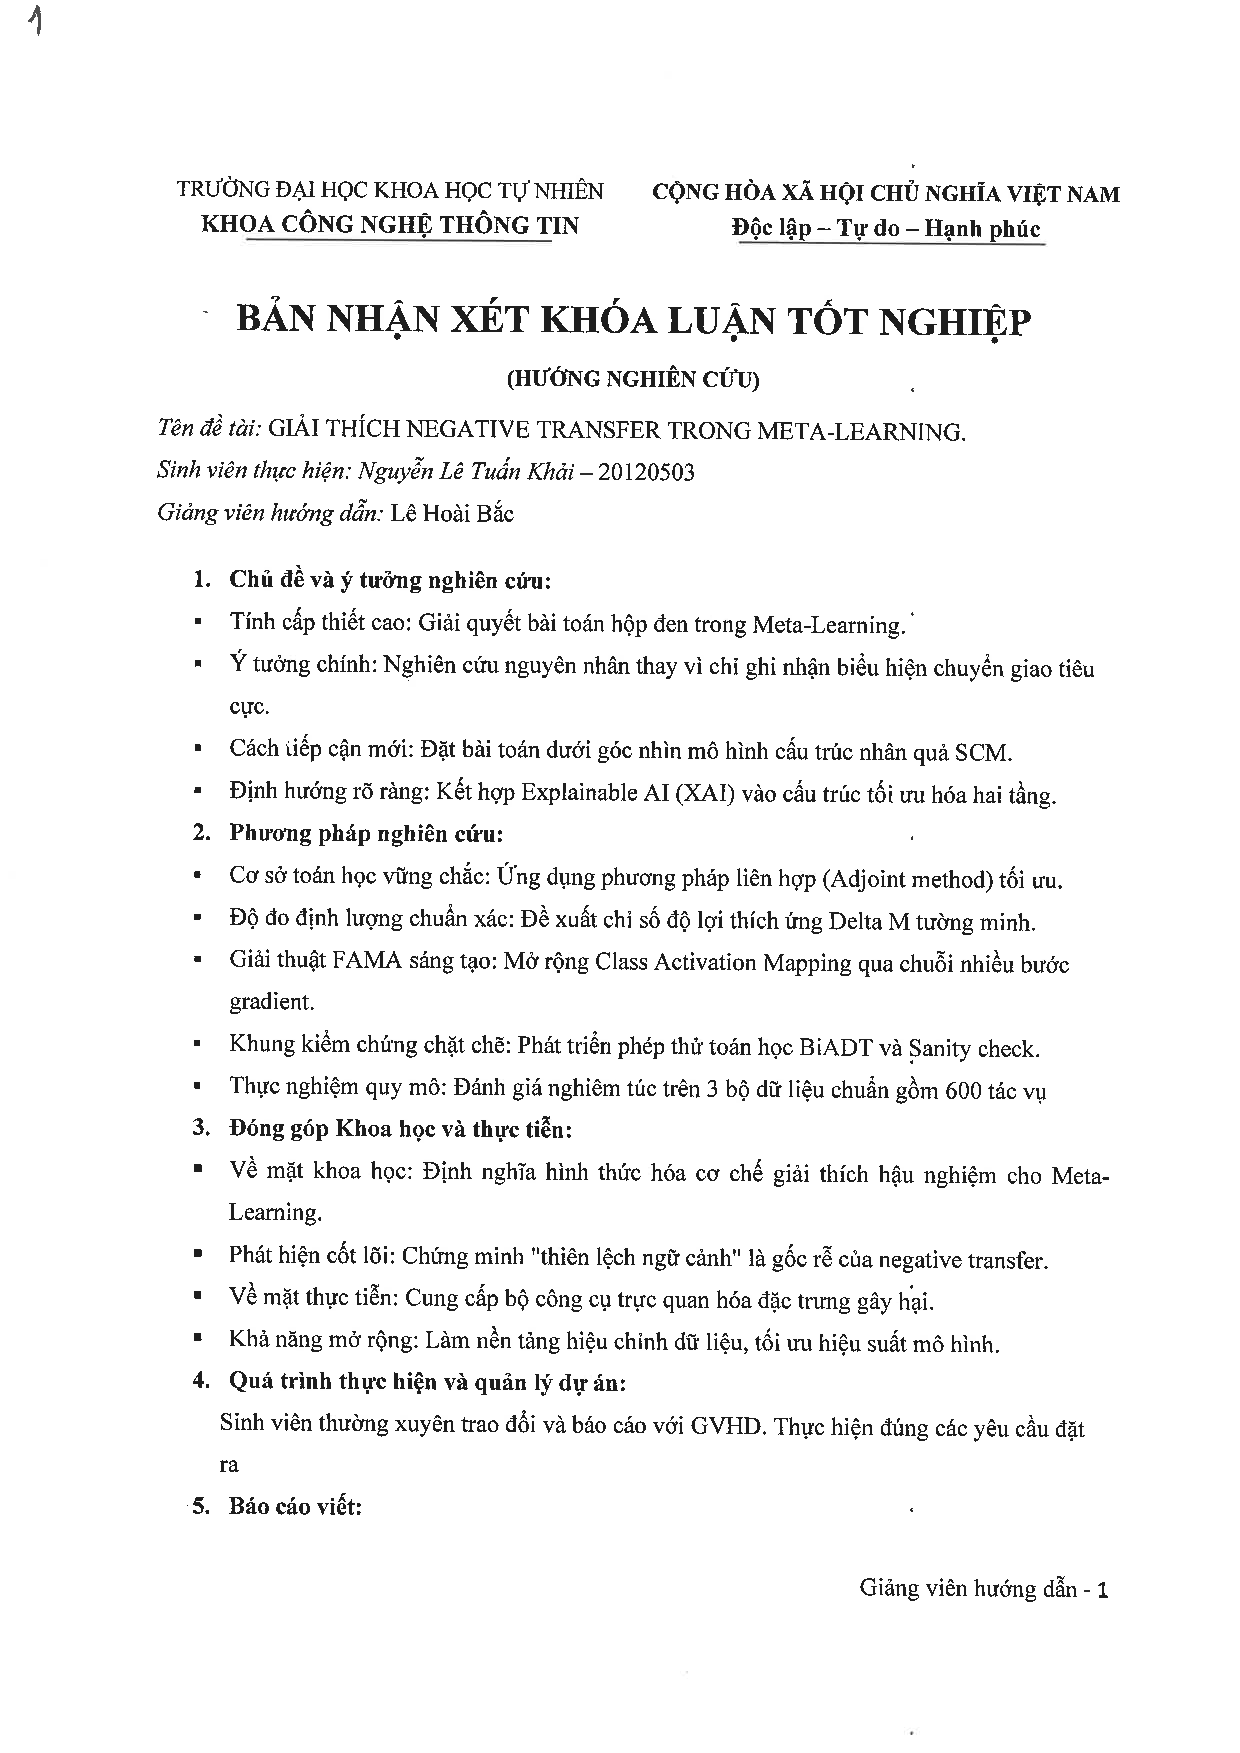
\includepdf[pages=-]{nhanxets.pdf}

\addcontentsline{toc}{chapter}{Lời cảm ơn}
\chapter*{Lời cảm ơn}
\label{thanks}

Trước hết, tôi xin được gửi lời tri ân sâu sắc nhất đến GS.TS. Lê Hoài Bắc, người đã tận tình hướng dẫn, định hướng và hỗ trợ tôi trong suốt quá trình thực hiện luận văn này. Những góp ý chuyên môn sâu sắc từ thầy chính là động lực to lơn giúp tôi hoành thành nghiên cứu này một cách trọn vẹn.

Bên cạnh đó, tôi cũng xin bày tỏ lòng kính trọng và biêt ơn sâu sắc đến tập thể giảng viên Khoa Công nghệ Thông tin, Trường Đại học Khoa học Tự nhiên - ĐHQG TP.HCM, đã truyền thụ cho tôi những nền tảng tri thức chuyên môn vững chắc trong suốt quá trình học tập tại trường. Chính những tri thức này đã định hình tư duy một cách hoàn thiện để đạt được các kết quả trong nghiên cứu này.

Cuối cùng, tôi muốn gửi lời cảm tạ tới gia đình, bạn bè đã luôn đồng hành cùng tôi trong suốt hành trình vừa qua.

Và lời kết, dù đã dành nhiều tâm huyết và nỗ lực, song đề án khó tránh khỏi những điểm thiếu sót ngoài ý muốn. Cho nên, tôi kính mong nhận được những lời nhận xét, góp ý quý báu từ quý thầy cô và Hội đồng để nghiên cứu này ngày càng hoàn thiện hơn.

Tôi xin trân trọng cảm ơn!


\addcontentsline{toc}{chapter}{Đề cương chi tiết}
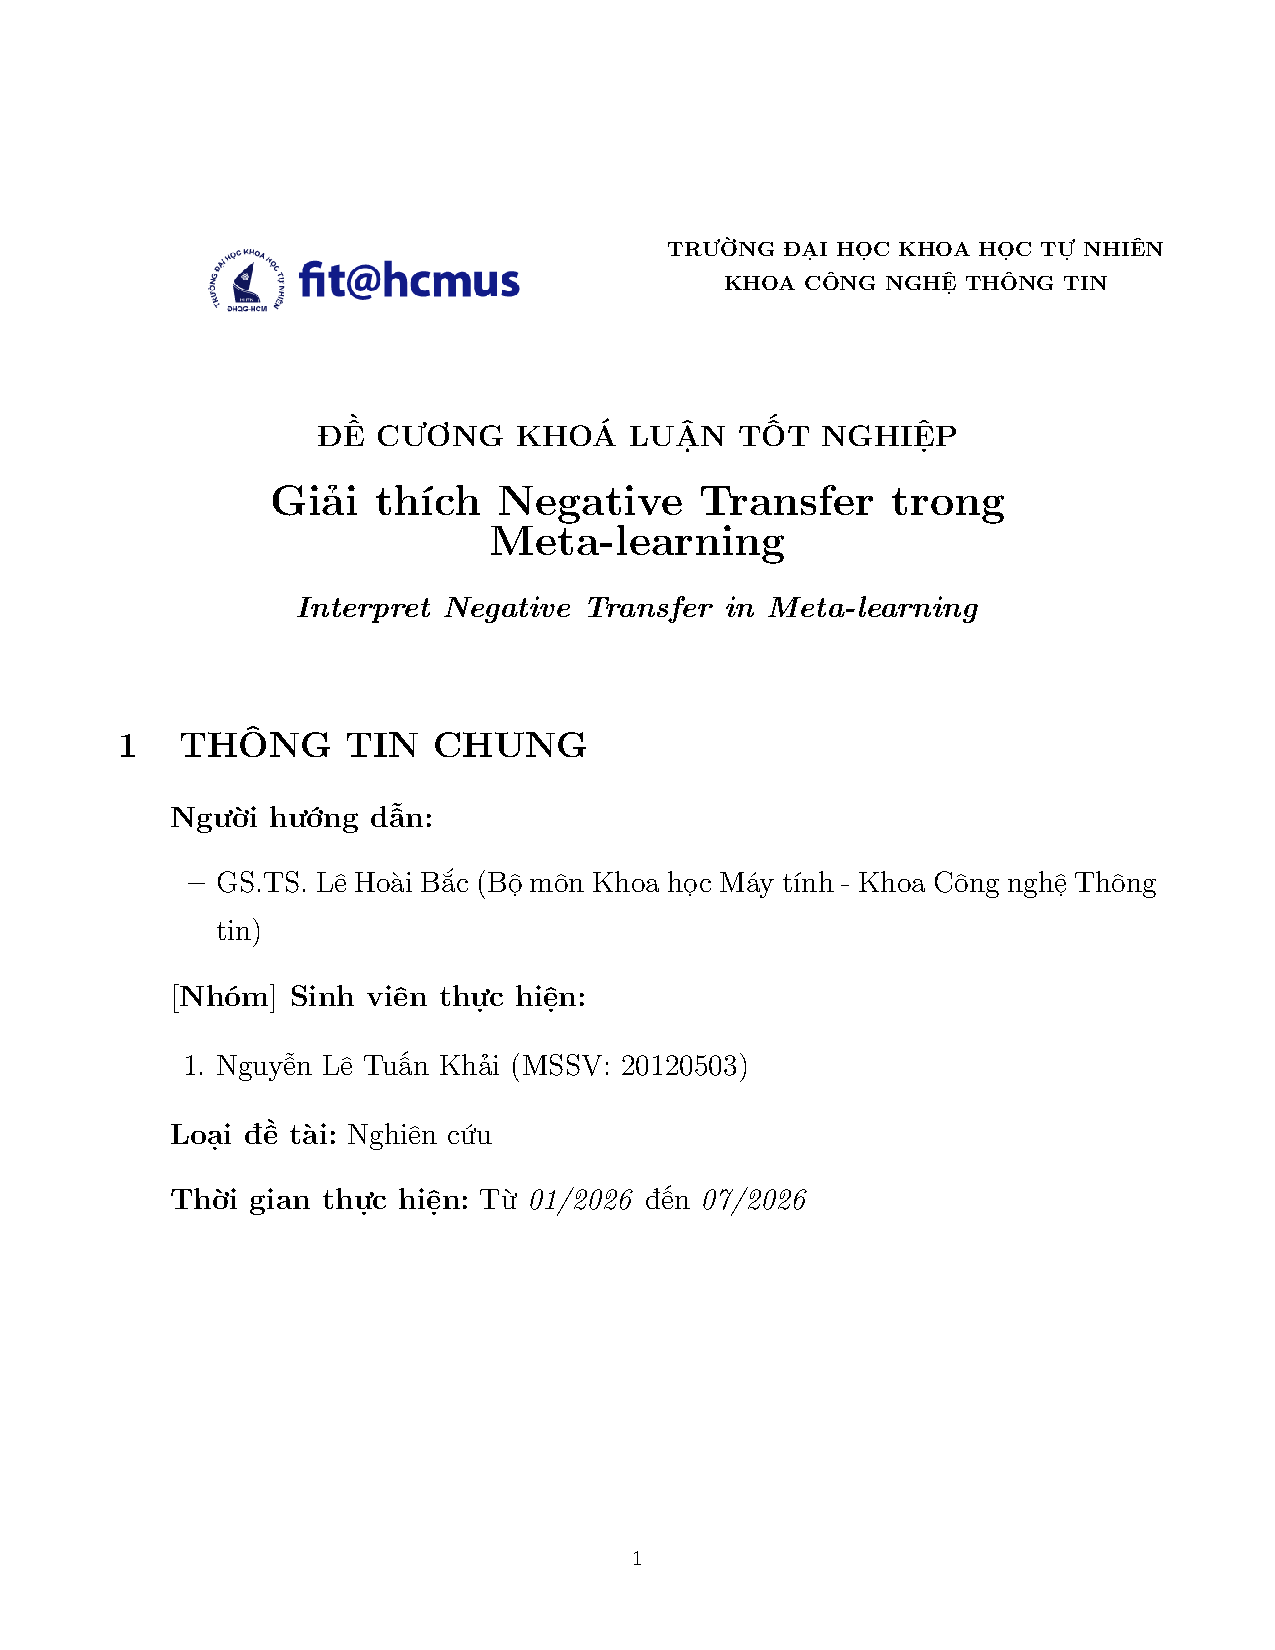
\includepdf[pages=-]{25D2-KL-KHMT03_DeCuong_16032026.pdf}

% Mục lục, danh sách hình, danh sách bảng
\addcontentsline{toc}{chapter}{Mục lục}
\printglossary[type=\acronymtype, title={Danh mục các từ viết tắt}]
\tableofcontents
\listoffigures
\listoftables

\addcontentsline{toc}{chapter}{Tóm tắt}
\chapter*{Tóm tắt}
\label{abs}

Học sâu hiện đại phụ thuộc nặng vào dữ liệu lớn, khiến các bài toán thiếu dữ liệu gán nhãn gặp nhiều trở ngại. Trong bối cảnh đó, meta-learning dựa trên gradient, tiêu biểu là MAML, nổi lên như hướng tiếp cận chủ đạo cho học ít mẫu. Tuy nhiên, cơ chế tri thức tiền nghiệm ở tham số khởi tạo $\theta_0$ chi phối quá trình thích ứng nhanh vẫn là hộp đen, khiến chuyển giao tiêu cực (negative transfer) - khi tập hỗ trợ $S_i$ định hướng sai làm giảm hiệu suất — chỉ được phát hiện qua các biểu hiện chứ chưa giải thích được ở cấp độ nguyên nhân. Đề tài đặt mục tiêu xây dựng phương pháp hậu diễn giải nhằm định lượng mức lợi/hại của bước thích nghi và định vị đặc trưng trong tập hỗ trợ gây ra ảnh hưởng đó. Trong đó, đề tài đề xuất độ lợi thích nghi $\Delta M$, đo bằng chênh lệch hàm mất mát trên tập truy vấn giữa hai nhánh can thiệp và không can thiệp quá trình thích ứng, cùng phương pháp \acrfull{fama} nhằm mở rộng Class Activation Mapping qua nhiều bước gradient để trực quan hóa đặc trưng có lợi/hại. Tính trung thực được kiểm định qua phép xóa-và-đo hai chiều và kiểm tra tỉnh táo, thực nghiệm trên kiến trúc Conv4 với \emph{miniImageNet}, \emph{tieredImageNet} và \emph{CUB-200-2011}. Kết quả cho thấy hai chỉ số $\mathrm{ABC}_\downarrow$, $\mathrm{ABC}_\uparrow$ đạt ý nghĩa thống kê (p<0,001), tương quan tỉnh táo sụt giảm gần như tức thời khi phá hủy tầng gần đầu ra, và phân tích trên 600 tác vụ chỉ ra "thiên lệch ngữ cảnh" là nguyên nhân cốt lõi gây chuyển giao tiêu cực. Kết quả khẳng định \acrshort{fama} là công cụ diễn giải trung thực, đáng tin cậy cho thích nghi trong meta-learning, mở ra ứng dụng chẩn đoán, giảm thiểu chuyển giao tiêu cực, và làm nền tảng mở rộng sang kiến trúc sâu hơn.


\clearpage

\pagenumbering{arabic} % Đánh số 1, 2, 3, ...

% Các chương nội dung
\chapter{Phần mở đầu}
\label{Chapter1}

\section{Tính cấp thiết của đề tài}
\label{sec:research_urgency}
Trong khoảng một thập kỷ trở lại đây, \acrfull{ml} nói chung và \acrfull{dl} nói riêng đã đạt được những thành tựu vượt bậc trên hầu hết các bài toán trong các lĩnh vực khác nhau. Tuy nhiên, phần lớn thành công này dựa trên một giả định rằng mô hình có thể được huấn luyện trên một tập dữ liệu có kích thước lớn và đa dạng cho tác vụ cụ thể, và nhìn chung, mô hình càng sâu thì càng khai thác tốt lượng dữ liệu đó để giải quyết tác vụ. Nhưng giả định này trong bối cảnh thực tế đã vấp phải một trở ngại lớn đối với nhiều tác vụ nhạy cảm hoặc đặc thù, việc thu thập một lượng dữ liệu đủ lớn và đa dạng là rất khó khăn, thậm chí bất khả thi, do chi phí, tính đặc thù chuyên môn (y khoa, công nghiệp) hoặc các ràng buộc đạo đức và pháp lý \cite{wang2020generalizing, fawakherji2026learning}.

Bài toán \acrfull{fsl} vốn đã được đặt nền móng từ trước khi \acrlong{dl} bùng nổ, nhưng trở nên đặc biệt cấp thiết trở lại trong kỷ nguyên deep learning, khi các mô hình sâu hiện đại lại càng phụ thuộc nặng nề vào dữ liệu lớn. Các phương pháp \acrshort{fsl} dựa trên deep learning ra đời nhằm giải quyết trực tiếp trở ngại này, cho phép mô hình học và tổng quát hóa tốt chỉ với một lượng rất nhỏ mẫu dữ liệu gán nhãn. Trong số các hướng tiếp cận của bài toán \acrlong{fsl}, Meta-Learning (học cách học) vốn đã được đề xuất từ lâu, trước cả deep learning hiện đại \cite{schmidhuber1987evolutionary, bengio2013optimization}, là hướng phổ biến và đặc trưng cho lớp bài toán này. Đồng thời, với đột phá của C.Finn và các cộng sự \cite{finn2017model}, lớp phương pháp dựa trên gradient (gradient-based), đại diện tiêu biểu là \acrfull{maml} đã trở thành một trong những hướng tiếp cận chủ đạo nhờ tính linh hoạt và khả năng áp dụng cho mọi kiến trúc khả vi.

Tuy nhiên, cũng như phần lớn các mô hình học sâu khác, các mô hình meta-learning nói chung và \acrshort{maml} nói riêng vẫn là các mô hình hộp đen (blackbox models). Cơ chế mà tri thức tiền nghiệm (prior knowledge) ẩn chứa trong bộ tham số khởi tạo $\theta_0$ chi phối quá trình thích nghi nhanh (fast-adaptation) trên tập hỗ trợ (support set) $S$ vẫn chưa được biểu diễn một cách tường minh. Sự thiếu minh bạch này đặt ra rào cản lớn khi triển khai các hệ thống đòi hỏi độ tin cậy cao, nơi người dùng cần kiểm chứng được quyết định của mô hình thay vì chấp nhận nó như một phép màu thống kê \cite{lum2016predict, angwin2016machine}.

Đồng thời, tri thức tiền nghiệm cũng không phải lúc nào cũng có lợi cho tác vụ đích. Khi tác vụ đích là một tác vụ không đồng nhất (Heterogeneous task), tập hỗ trợ của tác vụ đích khó (hard), nhiễu (noisy), hoặc nằm ngoài phân phối (out-of-distribution) so với phân phối các tác vụ tại giai đoạn meta-training \cite{si2025meta}, quá trình thích nghi nhanh có thể trở nên kém hiệu quả, thậm chí làm giảm hiệu suất so với trước khi thích nghi. Mà nguyên nhân chính dẫn tới việc giảm hiệu suất chính là do sự chuyển giao tiêu cực (negative transfer) của các tri thức tiền nghiệm (prior knowledge), vốn đã được Yue và các cộng sự chứng minh trong công trình của mình \cite{yue2020interventional}.

Nhưng hầu hết các phương pháp giải quyết hiện tượng chuyển giao tiêu cực hiện chỉ được \textbf{phát hiện thông qua triệu chứng} từ các độ đo về độ chính xác giảm trên tác vụ đích, chứ chưa được \textbf{giải thích ở cấp độ nguyên nhân}, do bản thân bước thích nghi vẫn là một hộp đen. Một kết quả khác do Raghu và các cộng sự \cite{raghu2019rapid} thực hiện việc đóng băng phần thân mạng (backbone) và chỉ thực hiện thích nghi nhanh với phần đầu ra (head) của mô hình, cho thấy phần lớn hiệu quả của \acrshort{maml} đến từ việc tái sử dụng đặc trưng (feature reuse) của phần thân mô hình (backbone) đã được học từ quá trình meta-training. Điều này gợi ý rằng tập hỗ trợ $S$ đóng một vai trò lớn trong việc định hướng tín hiệu thích nghi (steering signal) trên không gian đặc trưng sẵn có. Do đó, dẫn tới một góc nhìn khác là nguyên nhân của negative transfer nhiều khả năng nằm ở việc $S$ định hướng sai vùng chú ý của mô hình trong quá trình thích nghi nhanh. Hướng lập luận này được củng cố gián tiếp bởi HSFM \cite{parast2026hsfm}, phương pháp can thiệp trực tiếp lên các vector nhúng của tập hỗ trợ $S$ (support embeddings) trong không gian đặc trưng đã được đóng băng để chống tương quan giả. 

Tuy nhiên tất cả các phương pháp trên, chỉ dừng ở việc \textbf{sửa chữa} biểu diễn nhằm tăng cường hiệu suất khái quát hóa cho tác vụ đích, mà không nhằm \textbf{giải thích cho con người} cơ chế mà $S$ đã định hướng sai ở đâu. 

Ở một nhánh khác trong lĩnh vực nghiên cứu về \acrlong{ml}, \acrfull{xai} trong những năm gần đây đã được giới học thuật chú ý trở lại và đạt được nhiều thành công đáng kể trong việc mở hộp đen cho các mô hình học sâu đơn lẻ, tiêu biểu là các phương pháp diễn giải cục bộ (local explanation) như Grad-CAM \cite{selvaraju2017grad} hay SHAP \cite{lundberg2017unified}. Tuy nhiên, việc áp dụng các kỹ thuật này vào các phương pháp học có cấu trúc tối ưu hai tầng như meta-learning/\acrshort{maml} vẫn còn rất hạn chế. Các nỗ lực hiện có theo hướng này đối với dữ liệu phi cấu trúc nói chung và dạng hình ảnh nói riêng, chủ yếu chỉ diễn giải được bước suy luận cuối cùng trên mô hình đã thích nghi (Grad-CAM cục bộ \cite{uddin2025expert}), mà bỏ qua vai trò định hướng của tập hỗ trợ $S$. Và phương pháp gần đây nổi bậc do Mitsuka và các cộng sự đề xuất \cite{mitsuka2025tlxml} nhằm mở rộng hàm ảnh hưởng (influence functions) sang cấp độ tập hợp các tác vụ (task-level) để định lượng ảnh hưởng của các tác vụ trong quá trình meta-training ảnh hưởng lên hành vi thích nghi. Nhưng nhược điểm của phương pháp này là vẫn phụ thuộc vào dữ liệu các tác vụ trong quá trình huấn luyện để tính giá trị ảnh hưởng, gây cản trở lớn về mặt chi phí tính toán, đồng thời giới hạn khả năng áp dụng trong các ứng dụng thực tế nơi dữ liệu meta-training bị đóng gói hoặc không thể truy xuất do rào cản bảo mật.

Xuất phát từ khoảng trống trên, nghiên cứu này đặt ra câu hỏi trung tâm, \textit{điều gì gây ra negative transfer trong quá trình thích nghi của meta-learning?}. Câu hỏi này có thể được cụ thể hóa thành hai câu hỏi nghiên cứu theo thứ từ lần lượt. Thứ nhất, quá trình thích nghi từ tri thức tiền nghiệm (prior knowledge) sang tri thức cụ thể (specific knowledge) với một tác vụ đích cho trước là có lợi hay có hại, và mức độ ảnh hưởng đó là bao nhiêu? Thứ hai, những đặc trưng nào trong tập hỗ trợ $S$ là nguyên nhân gây ra ảnh hưởng tích cực hay tiêu cực đó, và chúng nằm ở đâu trong không gian đặc trưng $F$?

Để giải quyết và trả lời hai câu hỏi nghiên cứu này, không chỉ đòi hỏi một độ đo định lượng mà còn yêu cầu một cơ chế diễn giải hậu nghiệm nhằm truy vết ngược từ độ đo đó về từng đặc trưng đầu vào. 

\section{Mục tiêu nghiên cứu}
\label{sec:objective}
Xuất phát từ khoảng trống đã được phân tích ở phần \ref{sec:research_urgency} với hai câu hỏi nghiên cứu đã nêu, mục tiêu của đề tài hướng đến việc xây dựng một khung diễn giải hậu nghiệm (post-hoc explanation framework) gồm hai thành phần chính, cùng với các thực nghiệm chứng minh tính hiệu quả và độ tin cậy của khung phương pháp này.

Với mục tiêu thứ nhất, là xây dựng một độ đo định lượng ứng với thành phần đầu tiên trong khung diễn giải, nhằm xác định mức độ lợi/hại của bước thích nghi nhanh trên một tác vụ đích cụ thể. Đồng thời, độ đo này phải nhạy cảm với sự thay đổi của $S$, thay vì chỉ đo hiệu suất tổng thể như độ chính xác truyền thống.

Với mục tiêu thứ hai, là xây dựng một phương pháp diễn giải thông qua trực quan hóa nhằm định vị các đặc trưng trong $S$, ứng với vị trí trong không gian đặc trưng chung $F$, đóng góp tích cực hay tiêu cực cho độ lợi thích nghi đo được ở thành phần thứ nhất.

Cuối cùng, đề tài đặt mục tiêu là thông qua các thực nghiệm định lượng lẫn định tính trên các bộ dữ liệu và backbone chuẩn, nhằm minh chứng phương pháp được đề xuất là hiệu quả, chính xác (correctness) và đáng tin cậy (trustworthiness) trong việc phản ánh đúng cơ chế thích nghi.

\section{Phương pháp tiếp cận}
\label{sec:proposed_method}

Tương ứng với các mục tiêu đã nêu, nghiên cứu đề xuất hai giải pháp kế tiếp nhau, cùng hai phép kiểm định đảm bảo tính đúng đắn và đáng tin cậy của cả hai. Đối với mục tiêu thứ nhất, độ lợi thích nghi (adaptation gain) $\Delta M$ được xây dựng dựa trên chênh lệch giá trị mất mát trên tập truy vấn $Q$ tại thời điểm trước và sau khi thực hiện quá trình thích nghi nhanh, đóng vai trò vừa là câu trả lời định lượng câu hỏi nghiên cứu thứ nhất, vừa là hàm mục tiêu để truy vết nguyên nhân ở bước tiếp theo. Đối với mục tiêu thứ hai, dựa trên việc mở rộng kỹ thuật Class Activation Mapping sang nhiều bước gradient liên tiếp trong quá trình thích nghi, nhằm lan truyền ngược độ lợi thích nghi $\Delta M$ về từng đặc trưng trong tập hỗ trợ $S$ trên không gian đặc trưng chung, qua đó xác định đặc trưng nào có lợi, đặc trưng nào có hại cho quá trình thích nghi.

Cuối cùng, tính đúng đắn (correctness) của FAMA được kiểm định thông qua hai phép kiểm tra. Thứ nhất là \acrfull{biadt}, điều chỉnh từ các bài kiểm tra xóa-và-đo (deletion test) truyền thống sang bối cảnh động của quá trình thích nghi, nhằm kiểm chứng tính trung thực (faithfulness) của FAMA đối với hành vi thực của mô hình. Thứ hai là bài kiểm tra độ nhạy (sanity check) \cite{adebayo2018sanity}, được điều chỉnh để xác minh rằng các attribution do FAMA sinh ra thực sự phụ thuộc vào tham số đã học của mô hình, chứ không phải một phép biến đổi không mang thông tin của đầu vào.

\section{Đóng góp của đề tài}
\label{sec:contributions}

Trong khuôn khổ luận văn, đề tài mang lại các đóng góp chính sau. 

\textbf{Thứ nhất,} đề tài phát biểu negative transfer trong meta-learning như một bài toán diễn giải hậu nghiệm ở cấp độ đặc trưng cho \textit{bản thân quá trình thích nghi nhanh (fast-adaptation)}, thay vì chỉ là một triệu chứng đo bằng độ chính xác. Góc nhìn này khác với TLXML \cite{mitsuka2025tlxml} vốn vẫn coi bước thích nghi là một hộp đen và Grad-CAM cục bộ vốn chỉ diễn giải được bước suy luận cuối cùng trên mô hình đã thích nghi (Chương~\ref{Chapter3}).

\textbf{Thứ hai,} đề tài đề xuất độ lợi thích nghi $\Delta M$, là độ đo định lượng mức độ lợi/hại mà bước thích nghi mang lại trên một tác vụ đích cụ thể, làm cơ sở để phát hiện negative transfer một cách định lượng thay vì chỉ định tính (Chương~\ref{Chapter3}).

\textbf{Thứ ba,} đề tài đề xuất \acrfull{fama}, phương pháp trực quan hóa trực tiếp đặc trưng nào trong $S$ có lợi hay có hại cho quá trình thích nghi trên không gian đặc trưng chung, khác với HSFM \cite{parast2026hsfm} ở chỗ hướng đến diễn giải cho con người thay vì chỉ sửa chữa biểu diễn để tăng hiệu năng (Chương~\ref{Chapter3}).

\textbf{Thứ tư,} đề tài đề xuất \acrshort{biadt} và điều chỉnh phép sanity check sang bối cảnh thích nghi động. Hai công cụ này không phụ thuộc riêng vào \acrshort{fama} và có thể áp dụng để kiểm định bất kỳ phương pháp XAI nào khác được đề xuất trong tương lai cho bài toán thích nghi trong meta-learning (Chương~\ref{Chapter4}).

\section{Bố cục luận văn}
\label{sec:structure}
Phần còn lại của luận văn được tổ chức thành các chương như sau:

\begin{itemize}
    \item \textbf{Chương 2 - Tổng quan nghiên cứu}: trình bày nền tảng lý thuyết về \acrlong{fsl}, Meta-Learning, cơ chế thích nghi hai tầng của MAML, các phương pháp diễn giải hậu nghiệm dựa trên saliency map, và các nguyên lý kiểm định XAI (completeness, sanity check). Trên cơ sở đó, các phân tích và đánh giá của các công trình liên quan trực tiếp về cơ chế nội tại của MAML, và về XAI ở mức tác vụ (TLXML) hay feature-space (HSFM) sẽ được trình bày nhằm nêu rõ những vấn đề mà các hướng này chưa giải quyết được, từ đó chỉ ra những vấn đề mà đề tài tập trung giải quyết thông qua $\Delta M$ và FAMA.

    \item \textbf{Chương 3 - Phương pháp đề xuất}: phát biểu bài toán và trình bày chi tiết hai thành phần chính của đề tài. Gồm định nghĩa độ lợi thích nghi $\Delta M$ và phương pháp \acrfull{FAMA}, cơ sở toán học và ý nghĩa của chúng.

    \item \textbf{Chương 4 - Thực nghiệm và đánh giá}: mô tả thiết lập thực nghiệm trên các bộ dữ liệu chuẩn và các phương pháp đối chứng. Đồng thời, cũng trình bày các bài kiểm định tính đúng đắn và độ tin cậy của \acrshort{fama}, và phân tích kết quả định lượng lẫn định tính.

    \item \textbf{Chương 5 - Kết luận và hướng phát triển}: tổng kết các kết quả đạt được, hạn chế của phương pháp, và đề xuất hướng phát triển trong tương lai (mở rộng sang các phương pháp meta-learning khác ngoài MAML, sang các bài toán ngoài phân loại ảnh, và ứng dụng kết quả diễn giải vào việc giảm thiểu negative transfer trong quá trình huấn luyện).
\end{itemize}

%Ngôn ngữ để viết và trình bày báo cáo khóa luận tốt nghiệp, đồ án tốt nghiệp, thực tập tốt nghiệp (sau đây gọi chung là báo cáo) là tiếng Việt hoặc tiếng Anh. 
%Trường hợp chọn ngôn ngữ tiếng Anh để viết và trình bày báo cáo,  sinh viên cần có đơn đề nghị, được cán bộ hướng dẫn (CBHD) đồng ý và nộp cho bộ phận Giáo vụ của Khoa vào thời điểm đăng ký đề tài để xin ý kiến.
%Báo cáo viết và trình bày bằng tiếng Anh phải có bản tóm tắt viết bằng tiếng Việt.


%Tóm tắt luận văn được trình bày nhiều nhất trong 24 trang in trên hai mặt giấy, cỡ chữ Times New Roman 11 của hệ soạn thảo Winword hoặc phần mềm soạn thảo Latex đối với các chuyên ngành thuộc ngành Toán.

%Mật độ chữ bình thường, không được nén hoặc kéo dãn khoảng cách giữa các chữ.
%Chế độ dãn dòng là Exactly 17pt.
%Lề trên, lề dưới, lề trái, lề phải đều là 1.5 cm.
%Các bảng biểu trình bày theo chiều ngang khổ giấy thì đầu bảng là lề trái của trang.
%Tóm tắt luận án phải phản ảnh trung thực kết cấu, bố cục và nội dung của luận án, phải ghi đầy đủ toàn văn kết luận của luận án.
%Mẫu trình bày trang bìa của tóm tắt luận văn (phụ lục 1).

\chapter{Tổng quan nghiên cứu}
\label{Chapter2}

\section{Cơ sở lý thuyết}
\label{sec:background}
\subsection{Bài toán \acrfull{fsl} và Meta-Learning}

Bài toán \textbf{\acrfull{fsl}} khởi nguồn từ các công trình về one-shot learning dựa trên suy luận Bayesian, khai thác tri thức đã học từ các lớp đối tượng trước đó để nhận diện một lớp mới chỉ từ một hoặc vài mẫu quan sát \cite{fei2006one}. Khái niệm này ra đời từ trước khi \acrlong{dl} bùng nổ, nhưng đã trở nên đặc biệt cấp thiết trở lại trong kỷ nguyên deep learning và từ đó phát triển thành một nhánh nghiên cứu riêng với hàng loạt phương pháp dựa trên mạng nơ-ron sâu, tập trung xây dựng các mô hình có khả năng khái quát hóa mạnh mẽ trên các lớp hoặc tác vụ mới mà không cần thu thập lượng dữ liệu quy mô lớn \cite{wang2020generalizing}.

Về mặt hình thức, \acrshort{fsl} phổ biến nhất với bài toán $N$-way $K$-shot, nơi mô hình cần xử lý các tác vụ, phân biệt $N$ lớp, với điều kiện mỗi lớp chỉ có $K$ mẫu được gán nhãn. Để mô hình đạt được năng lực khái quát hoá này, quá trình huấn luyện được tổ chức theo cơ chế \emph{episodic training} trên một tập hợp các tác vụ nền (base tasks) phong phú, gọi là giai đoạn \emph{meta-training}. Hiệu suất của mô hình sau đó sẽ được kiểm chứng trên các tác vụ hoàn toàn mới, không trùng lặp với giai đoạn trước, giai đoạn này gọi là \emph{meta-testing}. Mỗi tác vụ $\mathcal{T}_i$ trong cả hai giai đoạn đều được phân tách thành hai tập con biệt lập, gồm tập hỗ trợ (support set) $S_i = \{(x_k^S, y_k^S)\}_{k=1}^{N\times K}$, đóng vai trò như một "cuốn sách giáo khoa" chỉ với vài mẫu để mô hình được phép quan sát và thích ứng nhanh chóng, và tập truy vấn (query set) $Q_i = \{(x_k^Q, y_k^Q)\}_{k=1}^{M}$, dùng để đánh giá năng lực của mô hình sau thích ứng.

Dựa trên cách thức khai thác tri thức tiền nghiệm (prior knowledge), \acrshort{fsl} thường được phân thành ba nhóm phương pháp chính \cite{wang2020generalizing, song2023comprehensive}: tăng cường dữ liệu (data augmentation/hallucination), học chuyển giao (transfer learning) và Meta-Learning. Trong đó, \textbf{Meta-Learning} hay còn gọi là "học cách học" tiếp cận bài toán bằng cách tối ưu hóa trên toàn bộ phân phối tác vụ $p(\mathcal{T})$ thay vì một tác vụ đơn lẻ. Mục tiêu của Meta-Learning là tìm kiếm một cơ chế thích ứng sao cho mô hình đạt được hiệu năng tối ưu trên tập truy vấn $Q_i$  sau khi đã tiếp nhận tín hiệu từ tập hỗ trợ $S_i$ của tác vụ $\mathcal{T}_i$ tương ứng.

Dựa trên thành phần được tối ưu ở cấp độ phân phối tác vụ, các phương pháp Meta-Learning được chia thành ba nhóm tiêu biểu \cite{gharoun2024meta}.

\textbf{Nhóm thứ nhất}, là các phương pháp \textbf{Metric-based} học trên không gian nhúng (embedding space) sao cho khoảng cách giữa các mẫu trong cùng một lớp được tối thiểu, với tiêu biểu là Matching Networks \cite{vinyals2016matching} và Prototypical Networks \cite{snell2017prototypical}. \textbf{Nhóm thứ hai}, là các phương pháp \textbf{Model-based} sử dụng kiến trúc bộ nhớ ngoài hoặc siêu mạng (hypernetwork) để trực tiếp sinh ra tham số cho tác vụ mới, mà tiêu biểu là Memory-Augmented Neural Networks \cite{santoro2016meta}. \textbf{Cuối cùng}, là các phương pháp \textbf{Optimization-based} thực hiện việc thích ứng một cách tường minh qua các bước cập nhật gradient trên tập hỗ trợ $S$. Đây cũng là nhóm phương pháp có liên quan mật thiết nhất đến luận văn này, với đại diện tiêu biểu là \acrshort{maml} do C.Finn và các cộng sự đề xuất \cite{finn2017model}.

\subsection{\acrfull{maml}}
\label{subsec:maml_define}

\textbf{\acrfull{maml}} \cite{finn2017model} là đại diện tiêu biểu và có ảnh hưởng nhất trong nhóm các phương pháp dựa trên tối ưu hoá. Tiếp nối thành công của \acrshort{maml} nhiều biến thể đã được đề xuất nhằm tối ưu hóa quá trình học như Reptile \cite{nichol2018first} (một xấp xỉ bậc một của MAML), Meta-SGD \cite{li2017meta} - tự động hóa việc học tốc độ học (learning rate) như một siêu tham số, ALFA \cite{baik2020meta} - học một cơ chế sinh siêu tham số thích ứng theo từng bước và từng tác vụ, Meta-Curvature \cite{park2019meta} - học một ma trận tiền điều kiện (preconditioner) để định hình lại hình học của không gian tham số trong inner loop, iMAML \cite{rajeswaran2019meta} - sử dụng định lý hàm ẩn để tránh phải lan truyền ngược qua toàn bộ quỹ đạo $T$ bước của inner loop. Mà điểm chung của toàn bộ các phương pháp dựa trên tối ưu hoá này là chúng đều thừa nhận vai trò trung tâm của tập hỗ trợ $S$ như một "lực định hướng" cho quá trình thích ứng thông qua quá trình tối ưu hai tầng (bi-level optimization) đối với bộ tham số khởi tạo chung (shared initialization parameters) $\theta_0$.

Cụ thể, để giải quyết bài toán \acrlong{fsl}, \acrshort{maml} dựa trên cảm hứng về cơ chế học tập của con người. Trong suốt cuộc đời, con người sử dụng tri thức tích lũy từ quá khứ để nắm bắt nhanh các cấu trúc đặc thù của một bài toán mới. Chẳng hạn, khi đối diện với các bài toán hình học lạ, con người tận dụng tri thức về số lượng cạnh, đỉnh hay tính chất bất biến của phép quay để truy xuất lời giải thay vì bắt đầu từ con số không (Hình \ref{fig:meta_learning_demos}).

\begin{figure}[h]
    \centering
    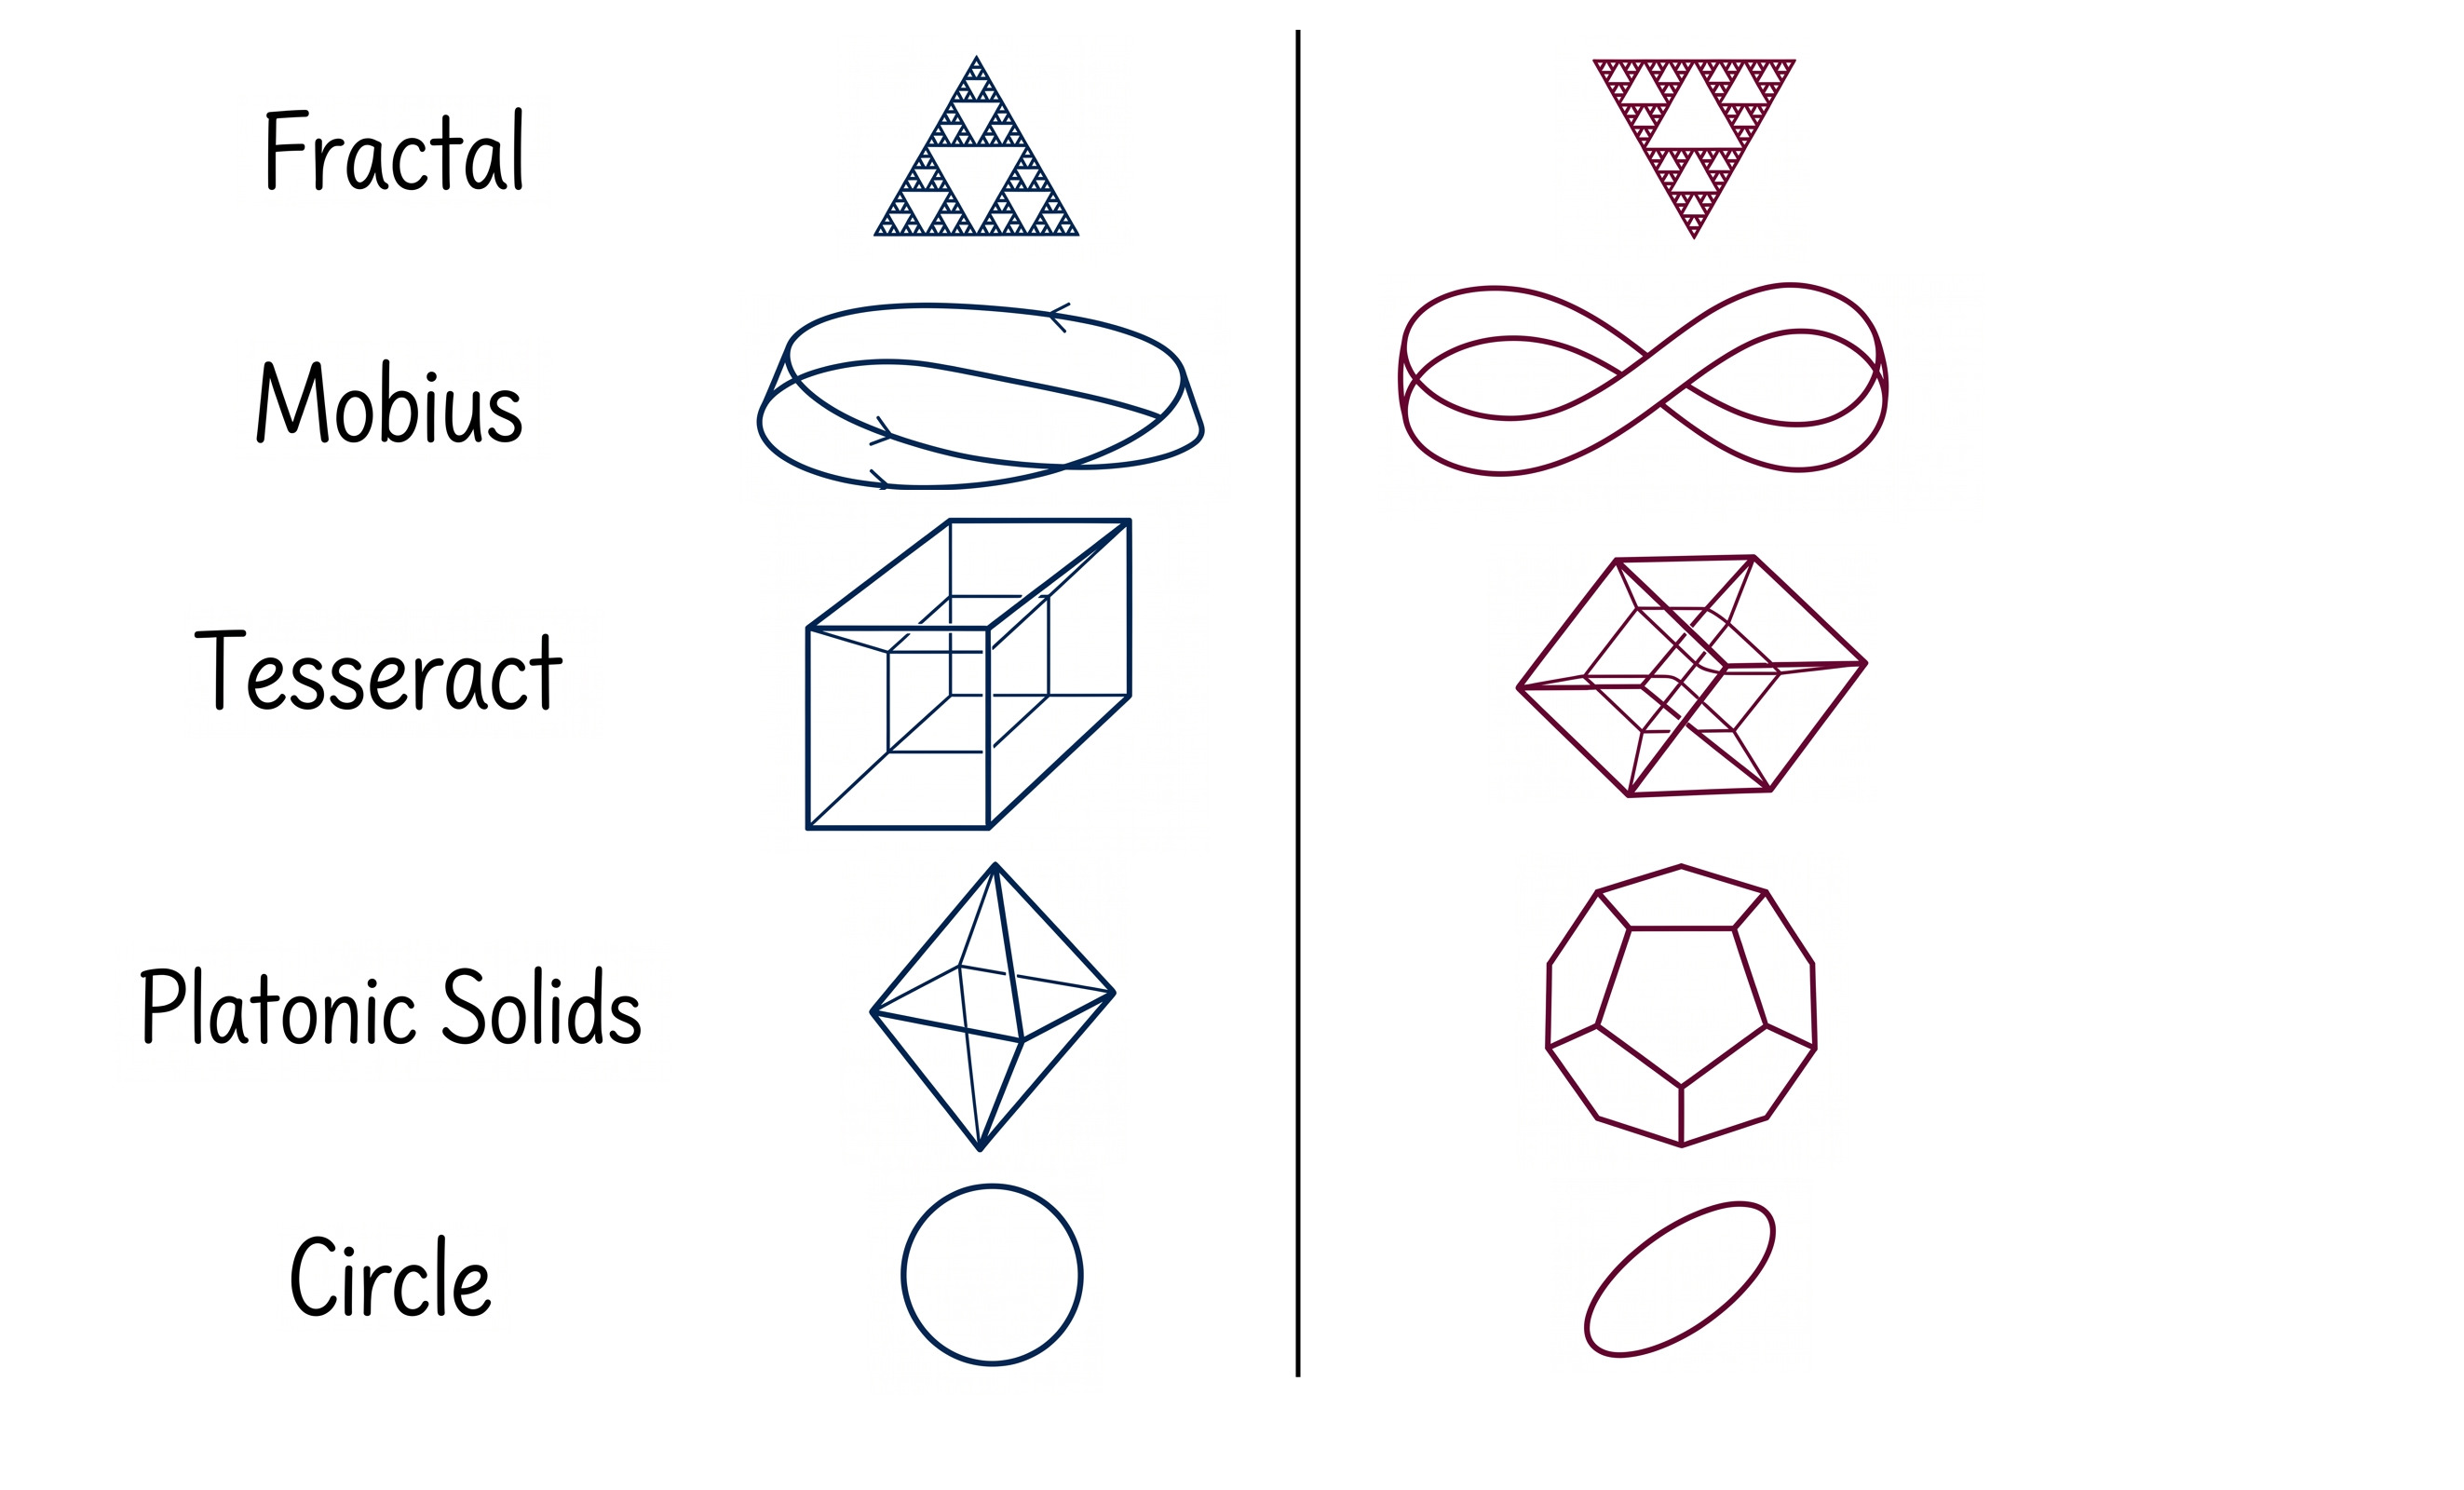
\includegraphics[width=0.8\textwidth]{../images/meta_learning_human.jpg}
    \caption{Hình minh họa một bài toán nhận diện hình học.}
    \label{fig:meta_learning_demos}
\end{figure}

Dựa trên cơ chế đó, \acrshort{maml} giải quyết bài toán \acrlong{fsl} thông qua một quá trình tối ưu gồm hai tầng (Hình \ref{fig:meta_learning_obj}). Với tầng lặp trong (inner loop), mô hình học xuất phát từ tham số khởi tạo chung $\theta_0$ thực hiện $T$ bước cập nhật gradient trên hàm mất mát tính trên tập hỗ trợ $S_i$ của tác vụ $\mathcal{T}_i$, theo phương trình \ref{eq:inner_loop}.
\begin{equation}
    \centering
    \phi_j = \phi_{j-1} - \alpha \nabla_{\phi} \mathcal{L}_{S_i}(\phi_{j-1}), \qquad j = 1, 2, \dots, T, \quad \phi{0} = \theta_0
    \label{eq:inner_loop}
\end{equation}
Trong đó $\alpha$ là tốc độ học của inner loop, và nghiệm sau $T$ bước được ký hiệu là $\phi_i^* := \phi_T$. Sau đó, ở tầng lặp ngoài (outer loop), tham số khởi tạo chung $\theta_0$ sẽ được cập nhật theo phương trình \ref{eq:outer_loop} sao cho tổng (hoặc trung bình) giá hàm mất mát trên các tập truy vấn $Q_i$, tính tại nghiệm đã thích ứng $\phi_i^*$, được tối thiểu hoá trên toàn bộ phân phối tác vụ.
\begin{equation}[h]
    \centering
    \theta = \theta_0 - \beta \nabla_\theta \sum_{k} \mathcal{L}_{Q_i}(\phi_i^*)
    \label{eq:outer_loop}
\end{equation}
Trong đó, $\beta$ là tốc độ học của outer loop, $\mathcal{L}_{Q_i}$ là hàm mất mát trên tập truy vấn $Q_i$ với mô hình sau khi cập nhật bởi inner loop và $\sum_{k}$ là tổng hàm mất mát của tất cả các tác vụ trong một meta-batch.

\begin{figure}[h]
    \centering
    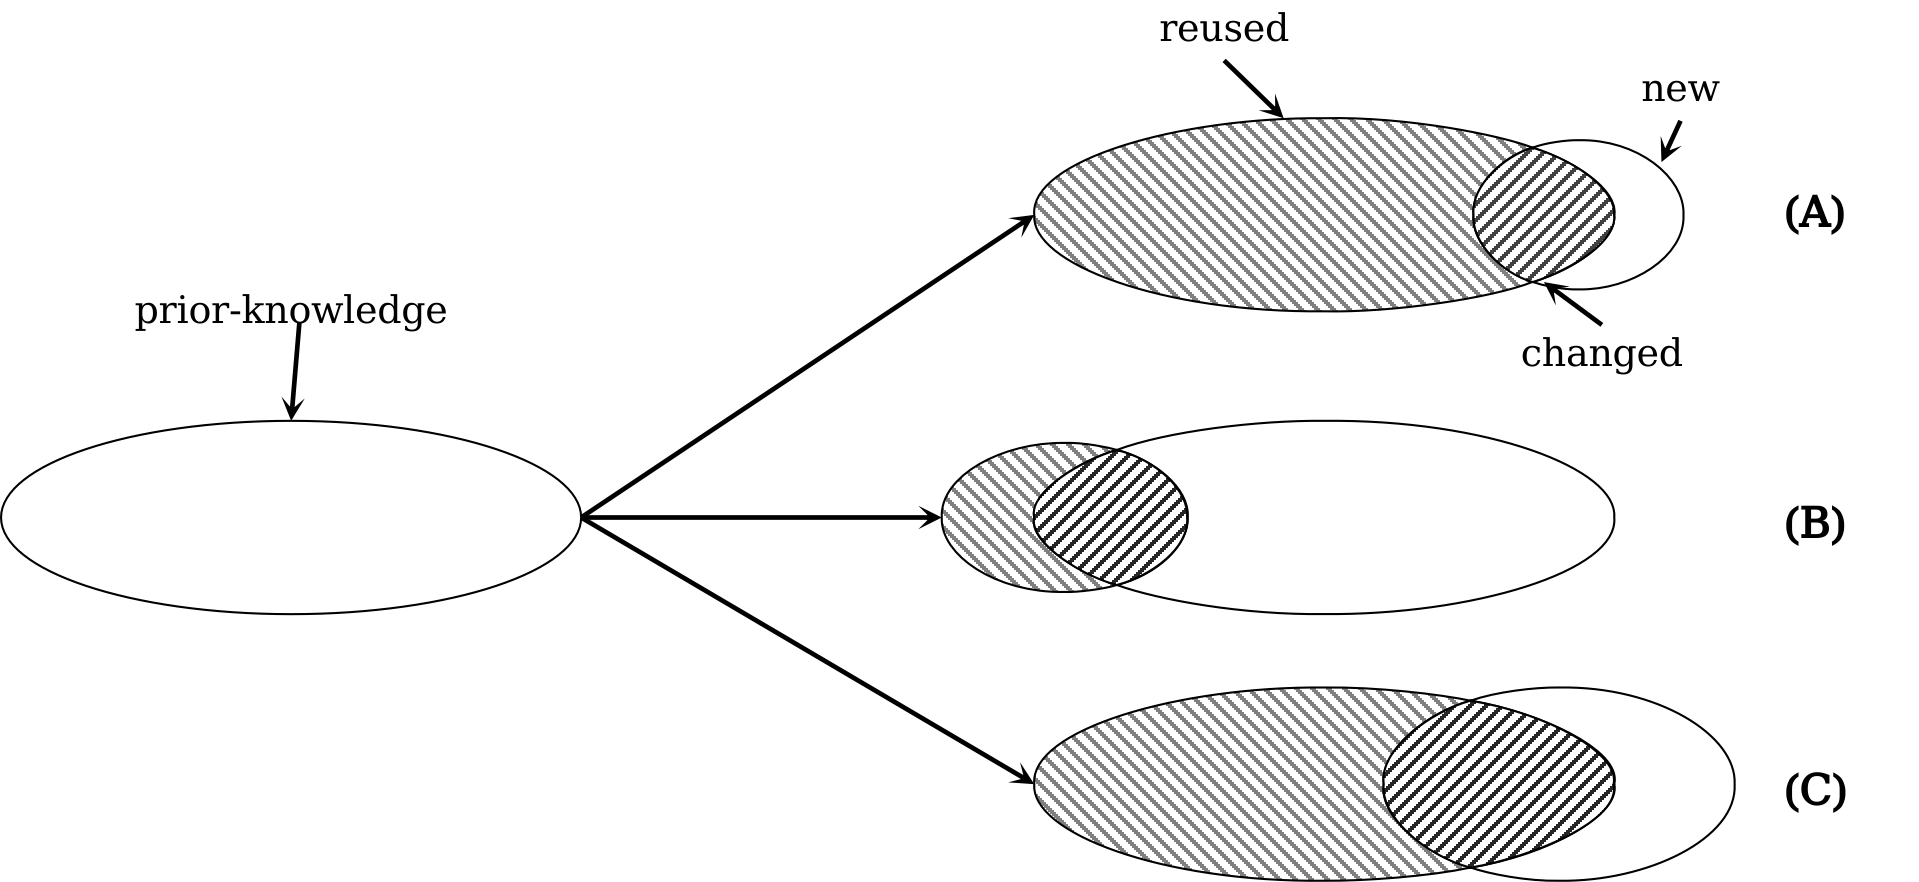
\includegraphics[width=0.8\textwidth]{../images/meta_learning_obj.png}
    \caption{Quá trình \acrshort{maml} tìm kiếm vị trí khởi tạo thuận lợi cho tham số $\theta_0$ trong giai đoạn meta-training.}
    \label{fig:meta_learning_process}
\end{figure}

Để lý giải cơ thích ứng nhanh của \acrshort{maml}, Raghu và các cộng sự \cite{raghu2019rapid} đã thực hiện thí nghiệm đóng băng phần thân trích xuất đặc trưng (backbone) $\theta_0^{b}$ và chỉ cho phép phần đầu phân loại (head) $\theta_0^{h}$ cập nhật trong inner loop - thuật toán ANIL (Almost No Inner Loop). Bằng cách so sánh biểu diễn của backbone trước và sau thích ứng thông qua CCA và CKA, nhóm tác giả cho thấy các lớp tích chập gần như không dịch chuyển, trong khi chỉ riêng head thay đổi đáng kể. Từ đó, đi tới kết luận rằng hiệu quả của \acrshort{maml} chủ yếu đến từ việc $\theta_0$ đã sẵn mang những đặc trưng tổng quát, có thể tái sử dụng nguyên trạng các đặc trưng này cho hầu hết tác vụ mới (feature reuse). Trạng thái này được khái quát hóa tại Hình \ref{fig:repr_space} A, trong đó không gian biểu diễn sau thích ứng ($\phi_i^*$) duy trì sự đồng nhất gần như tuyệt đối với không gian tiền nghiệm ($\theta_0$). Cũng đồng nghĩa với việc vai trò thực sự của $S_i$, trong trường hợp này, chỉ là căn chỉnh lại ranh giới quyết định ở phần đầu phân loại (head) cho phù hợp với từng tác vụ cụ thể.

Mặc dù vậy, giả thuyết về tính phổ quát của việc \emph{tái sử dụng đặc trưng (feature reuse)} bộc lộ sự hạn chế khi đối mặt với sự dịch chuyển phân phối (distribution shift) lớn giữa miền dữ liệu huấn luyện (meta-training) và miền kiểm tra (meta-testing). Oh và các cộng sự \cite{oh2020boil} đã phản bác hệ quả của ANIL thông qua một can thiệp kiến trúc đối xứng mang tên BOIL (Body Only Inner Loop) — chỉ cập nhật $\theta_0^{b}$ và đóng băng $\theta_0^{h}$. Kết quả là trên các môi trường có miền dữ liệu khác nhau (cross-domain), tri thức tiền nghiệm $\theta_0$ không chứa sẵn các biễu diễn có lợi và phù hợp cho tác vụ đích buộc phải dưới áp lực của $S_i$ dần bị thu hẹp và bị triệt tiêu tối đa, nhường chỗ cho sự dịch chuyển và hình thành các vùng biểu diễn hoàn toàn mới (Hình \ref{fig:repr_space} B). 

Từ sự đối lập của hai cơ chế trên, có thể thấy \acrshort{maml} tiêu chuẩn khi không bị ràng buộc bởi việc đóng băng trên toàn bộ mạng, đã cho phép nó hoạt động dựa trên một trạng thái linh hoạt điều chỉnh tỷ trọng giữa việc "tái sử dụng" và "tái cấu trúc". Lập luận này được củng cố bởi các thí nghiệm do Gou và các cộng sự thực hiện kiểm chứng trên các tập dữ liệu có sự khác biệt lớn, với kết luận tỷ trọng biến đổi của phần thân (backbone) tỷ lệ thuận với khoảng cách phân phối dữ liệu (domain shift). Hệ quả là, không gian biểu diễn chung $F$ của \acrshort{maml} sau khi thích ứng trở thành một môi trường giao thoa phức hợp bao gồm ba miền, (1) miền kế thừa nguyên trạng từ $\theta_0$, (2) miền đặc trưng cũ bị bẻ cong/điều biến dưới áp lực của $S_i$, và (3) miền tiếp thu các cấu trúc hoàn toàn mới (Hình \ref{fig:repr_space} C).

\begin{figure}[h]
    \centering
    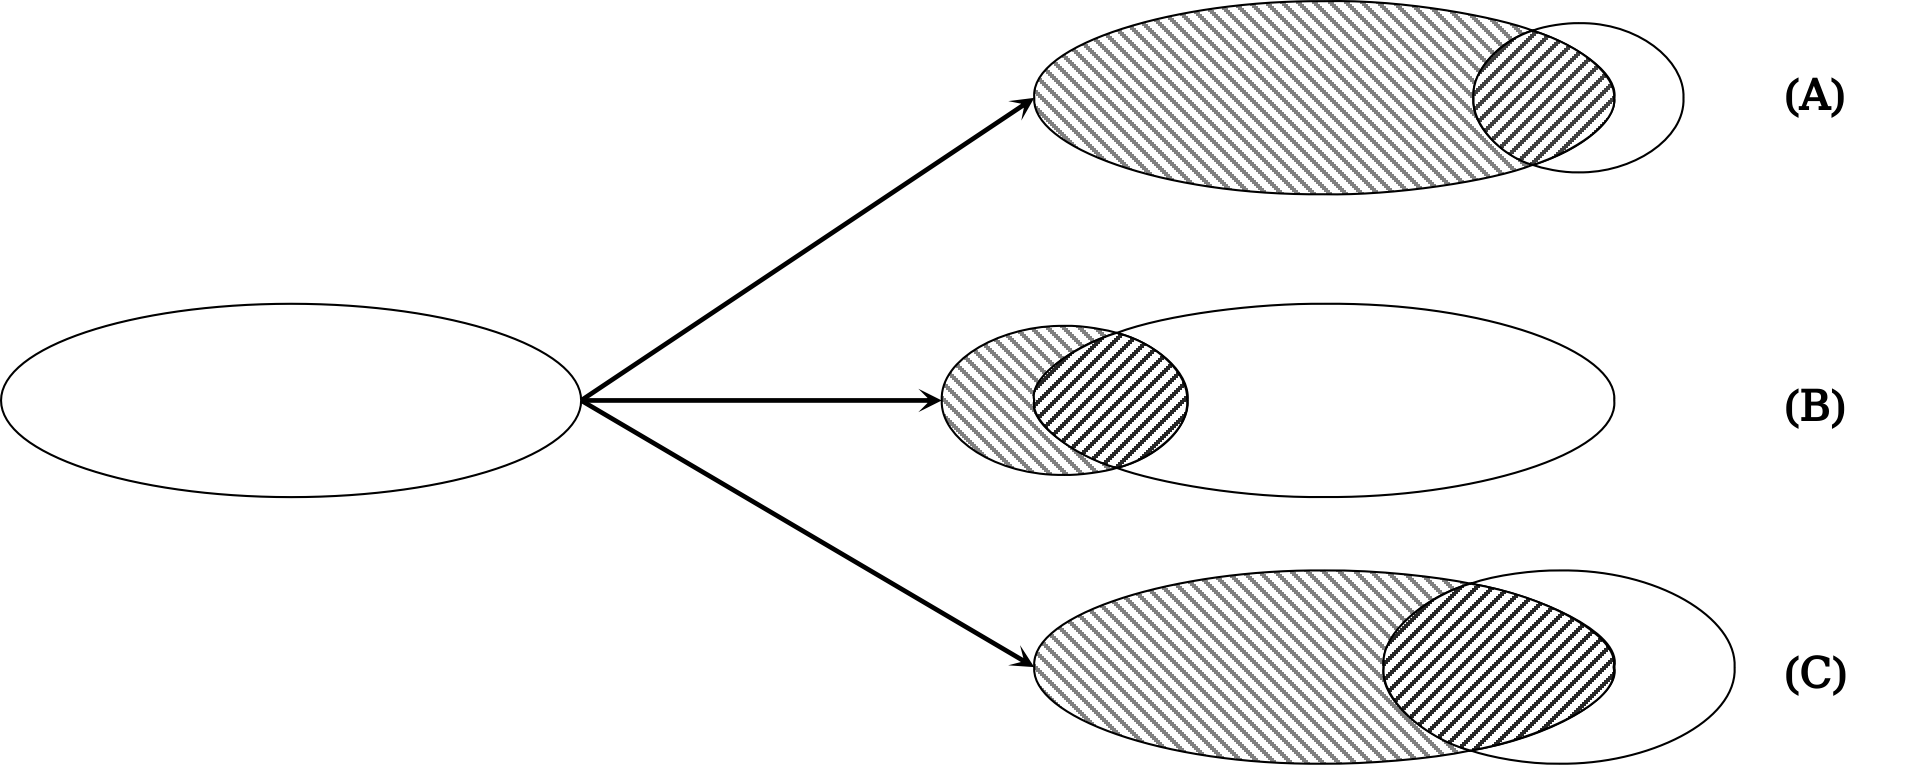
\includegraphics[width=\textwidth]{images/repr_space.png}
    \caption{Minh họa sự thay đổi của không gian biểu diễn $F$ sau thích ứng nhanh.}
    \label{fig:repr_space}
\end{figure}

\subsection{\acrfull{xai}}
\label{subsec:xai_bg}

Mặc dù \acrshort{maml} và các biến thể đã chứng minh được hiệu quả trong việc cải thiện \emph{phương thức} thích ứng, cơ chế vận hành của "lực định hướng" này tại cấp độ đặc trưng vẫn là một dạng "hộp đen". Các phương pháp hiện nay chưa cung cấp một lý giải tường minh cho câu hỏi: \textit{Tại sao một tập hỗ trợ cụ thể lại điều hướng mô hình tới một hướng thích ứng nhất định?} Sự thiếu vắng này đặc biệt đáng chú ý tại không gian đặc trưng chung $F$. Dẫn đến việc chúng ta không thể truy vết được nguồn gốc của các tương quan giả khi mô hình rơi vào trạng thái chuyển giao tiêu cực (negative transfer).

\textbf{\acrfull{xai}} là lĩnh vực nghiên cứu các phương pháp giúp con người hiểu được cơ chế ra quyết định của một mô hình học máy, ra đời như một phản ứng tất yếu trước sự phát triển của các mô hình học sâu. Trong khi các mô hình như hồi quy tuyến tính hay cây quyết định vốn có tính minh bạch nội tại (intrinsic model), cho phép truy vết trực tiếp đường đi từ đặc trưng đầu vào đến dự đoán đầu ra, thì các kiến trúc phức tạp hơn như mạng nơ-ron sâu lại đánh đổi tính minh bạch đó để lấy độ chính xác, trở thành những mô hình "hộp đen" mà cơ chế nội tại không thể quan sát trực tiếp.

Dựa trên thời điểm can thiệp vào mô hình, các kỹ thuật \acrshort{xai} được chia thành hai nhóm. \emph{Ante-hoc}, với tính khả diễn giải được tích hợp ngay từ khi thiết kế kiến trúc mô hình (cây quyết định, cơ chế attention, Self-Explaining Neural Networks) và \emph{post-hoc}, với các kỹ thuật diễn giải được áp dụng ngay sau khi mô hình đã huấn luyện xong, nhằm phân tích và diễn giải một mô hình đã có mà không cần huấn luyện lại. Do các phương pháp post-hoc không yêu cầu thay đổi kiến trúc hay quy trình huấn luyện gốc của mô hình, nên chúng có tính linh hoạt cao và có thể áp dụng cho các mô hình hộp đen phức tạp đã được huấn luyện. Theo Arrieta và các cộng sự \cite{arrieta2020explainable}, các kỹ thuật post-hoc thường dựa trên một trong ba cách tiếp cận chính. Gồm, đơn giản hoá mô hình (model simplification, xây dựng một mô hình thay thế — surrogate — dễ diễn giải hơn để xấp xỉ hành vi cục bộ của mô hình hộp đen, như LIME), độ liên quan đặc trưng (feature relevance explanation, xếp hạng mức độ quan trọng của từng đặc trưng đầu vào đối với một dự đoán cụ thể, như SHAP) và cuối cùng là trực quan hoá (visual explanation, cho phép con người quan sát trực tiếp bằng hình ảnh cơ chế mà mô hình đưa ra quyết định).

Trong ba hướng trên, trực quan hoá cho phép con người dễ dàng diễn giải lựa chọn của mô hình thông qua hình ảnh trực quan thay vì các con số trừu tượng. Tiêu biểu đối với các mạng nơ-ron tích chập (CNN) dùng cho các bài toán thị giác máy tính, các kỹ thuật trực quan hoá mức độ đóng góp (attribution visualization) đã được phát triển nhằm định vị và làm nổi bật những vùng đầu vào chi phối mạnh nhất đến kết quả dự đoán của mô hình. Khởi nguồn cho hướng tiếp cận này là bản đồ nổi bật (saliency map) của Simonyan và các cộng sự \cite{simonyan2014visualising}, sử dụng đạo hàm điểm ảnh (vanilla gradient) ứng với một lớp mục tiêu để sinh ra bản đồ có cùng kích thước không gian với ảnh đầu vào, qua đó định lượng trực tiếp mức độ đóng góp của từng vị trí vào quyết định của mô hình. Kế thừa nền tảng này, Guided Backpropagation \cite{springenberg2014striving} sau đó đã điều chỉnh lại quy tắc lan truyền ngược qua hàm kích hoạt ReLU nhằm triệt tiêu các gradient âm, từ đó tạo ra bản đồ phân bổ sắc nét hơn, dù vẫn bị giới hạn ở các điểm ảnh riêng lẻ. Nhằm dịch chuyển trọng tâm phân tích sang các vùng không gian ngữ nghĩa, Zhou và các cộng sự \cite{zhou2016learning} đề xuất Class Activation Mapping (CAM) bằng cách chèn thêm lớp global average pooling vào cuối kiến trúc mạng. Tuy nhiên, đổi lại CAM đòi hỏi phải thay đổi kiến trúc gốc và huấn luyện lại mô hình. Để khắc phục điểm nghẽn này, Gradient-weighted Class Activation Mapping (Grad-CAM) \cite{selvaraju2020grad} đã tổng quát hoá CAM, cho phép áp dụng hậu diễn giải (post-hoc) trên mọi mạng CNN mà không cần can thiệp kiến trúc. Bằng cách tận dụng gradient của lớp mục tiêu lan truyền ngược đến lớp tích chập cuối cùng, Grad-CAM đã tổng hợp thành một bản đồ nhiệt không gian, một đặc tính vô cùng giá trị khi làm việc với các mô hình đã huấn luyện sẵn. Mặc dù vậy, một điểm mù cố hữu của toàn bộ các biến thể CAM là việc trích xuất tín hiệu diễn giải luôn bị bó hẹp tại một \emph{trạng thái tham số tĩnh} duy nhất, tức thời điểm suy luận sau khi mạng đã hội tụ. Đặc tính tĩnh này khiến chúng trở nên bất lực khi phải giải phẫu hệ động lực học của quá trình thích ứng nhanh (fast adaptation), nơi không gian biểu diễn không đứng yên mà liên tục biến thiên qua từng bước cập nhật gradient.

\subsection{Correctness và trustworthiness của một phương pháp XAI}

Theo Hướng dẫn Đạo đức cho AI Đáng tin cậy (Ethics Guidelines for Trustworthy AI) của Nhóm chuyên gia cấp cao về AI thuộc Ủy ban Châu Âu (EC) \cite{eu2019trustworthy}, tính minh bạch (transparency), bao hàm khả năng diễn giải (explainability), là một trong bảy yêu cầu tiên quyết để kiến tạo một hệ thống AI đáng tin cậy (\emph{trustworthy}). Dẫu vậy, cần phân định rạch ròi giữa hai cấp độ khái niệm: "đáng tin cậy" là thuộc tính vĩ mô của \emph{toàn bộ hệ thống}, trong khi một phương pháp XAI, để đóng góp vào thuộc tính này, trước hết phải tự chứng minh được \textbf{tính đúng đắn} (\emph{correctness}) nội tại. Cụ thể, điều này đòi hỏi mức độ trung thành (\emph{faithfulness}) tuyệt đối của lời giải thích đối với cơ chế ra quyết định thực tế của mô hình, hoàn toàn độc lập với việc lời giải thích đó "nhìn có vẻ hợp lý" dưới lăng kính trực giác cảm quan của con người.

Để định lượng tính trung thành này, \textbf{nguyên lý thứ nhất} được thiết lập dựa trên kỹ thuật nhiễu loạn đặc trưng, nổi bật là phép kiểm định \emph{xóa-và-đo} (deletion test) do Samek và các cộng sự \cite{samek2016evaluating} đặt nền móng. Với ý tưởng cốt lõi là nếu bản đồ phân bổ định vị chuẩn xác các vùng đầu vào mang tính quyết định, thì việc tuần tự che khuất các vùng này (bằng nhiễu hoặc giá trị nền) theo thứ tự độ quan trọng giảm dần sẽ khiến hiệu năng dự đoán của mô hình suy sụp nhanh hơn đáng kể so với việc xóa ngẫu nhiên. Kế thừa tư tưởng này, Petsiuk và các cộng sự \cite{petsiuk2018rise} đã tiêu chuẩn hóa thành hai độ đo nghịch đảo — \emph{Xóa (Deletion)} và \emph{Thêm (Insertion)} — cho phép đánh giá khách quan tính trung thành thông qua diện tích dưới đường cong (AUC) của biểu đồ hiệu năng, qua đó triệt tiêu hoàn toàn sự phụ thuộc vào sự phán xét chủ quan của mắt người.

\textbf{Nguyên lý thứ hai}, được biết đến qua các phép kiểm tra tính hợp lý (sanity checks) do Adebayo và các cộng sự \cite{adebayo2018sanity} đề xuất, lại tập trung vào khả năng phản chiếu tri thức. Nguyên lý này lập luận, "một bản đồ phân bổ đích thực phải thể hiện sự \emph{nhạy cảm} trước những biến động phá vỡ cấu trúc tri thức tiềm ẩn của mạng". Thông qua kỹ thuật ngẫu nhiên hóa tham số lan truyền ngược từ lớp đầu ra (\emph{cascading randomization}), nhóm tác giả chỉ ra việc nếu bản đồ phân bổ gần như bất biến dù trọng số mô hình đã bị phá hủy ngẫu nhiên, phương pháp \acrshort{xai} đó thực chất không trích xuất bất kỳ tri thức nào, mà chỉ đang hoạt động như một bộ dò biên cạnh (edge detector) vô tri. Nghiên cứu này đã phơi bày một lỗ hổng nghiêm trọng của nhiều phương pháp \acrshort{xai} phổ biến thời bấy giờ (như Guided Backpropagation) khi chúng hoàn toàn trơ lỳ trước các lớp trọng số bậc cao, một "tử huyệt" bị che đậy đằng sau hình thức trực quan bắt mắt.

Tuy nhiên, như đã phân tích trước đó, dù cả hai nguyên lý trên đều cung cấp một khung đánh giá vững chắc, nhưng cũng đều tồn tại một điểm mù cố hữu. Chúng được thiết kế độc quyền cho các kiến trúc mô hình \emph{tĩnh}, nơi tín hiệu diễn giải được trích xuất từ một trạng thái tham số bất động tại một thời điểm suy luận duy nhất. Khi áp đặt vào hệ động lực học của quá trình thích ứng nhanh (fast-adaptation), nơi các bản đồ phân bổ được trích xuất liên tục chạy dọc theo một quỹ đạo cập nhật gradient, tính hiệu lực của các nguyên lý này lập tức bị thách thức. Bài toán làm thế nào để định lượng tính trung thành của một diễn giải XAI không chỉ tại một tọa độ tĩnh, mà xuyên suốt \emph{một chuỗi các biến thiên tham số liên tiếp}, hiện vẫn là một "vùng tối" chưa có lời giải trong cộng đồng nghiên cứu, đòi hỏi một nỗ lực tái định chuẩn và mở rộng hệ thống đo lường toàn diện.

\section{Các nghiên cứu liên quan}

Dựa trên nền tảng lý thuyết ở Mục~\ref{sec:background}, chúng tôi tiến hành rà soát bốn nhóm nghiên cứu liên quan trực tiếp đến đề tài. Gồm, các phương pháp hiện có giải quyết bài toán tác vụ không đồng nhất (heterogenous task) và hiện tượng Negative Transfer (Mục \ref{subsec:negative_transfer}), các công cụ hiện có cho hậu diễn giải (post-hoc) tổng quát dựa trên gradient và nhiễu loạn (perturbation) (Mục \ref{subsec:background_post_hoc}), khảo sát các phương pháp diễn giải hiện đang áp dụng riêng cho meta-learning (Mục \ref{subsec:xai_metalearning}) và attribution dựa trên quỹ đạo tham số (Mục \ref{subsec:trajectory_attribution}). Mục~\ref{subsec:relatedwork_synthesis} tổng hợp lại toàn bộ và chỉ ra các khoảng trống còn tồn tại.

\subsection{Tác vụ không đồng nhất (heterogeneous task) và hiện tượng Negative Transfer}
\label{subsec:negative_transfer}

Phần lớn các phương pháp meta-learning giả định ngầm rằng tập hợp tác vụ dùng để meta-training tương đối đồng nhất (\emph{homogeneous}), sao cho một điểm khởi tạo chung $\theta_0$ duy nhất là đủ tốt cho mọi tác vụ \cite{finn2017model, snell2017prototypical, vinyals2016matching, santoro2016meta}. Một nhánh nghiên cứu song song đã chỉ ra giả định này thường bị vi phạm trong thực tế, khi các tác vụ đích đến từ phân phối tác vụ không đồng nhất (task heterogenous) với phân phối tác vụ trong giai đoạn meta-training. Dẫn đến sự ra đời của các cơ chế tùy chỉnh (customize) tri thức tiên nghiệm theo từng cụm hoặc nhóm tác vụ thay vì chia sẻ toàn cục.

Yao và các cộng sự đã đề xuất \acrfull{hsml} \cite{yao2019hierarchically}, tổ chức các tác vụ thành một cấu trúc phân cụm phân cấp, qua đó đặc thù hóa tri thức chuyển giao cho từng nhóm tác vụ thay vì buộc mọi tác vụ chia sẻ một tri thức toàn cục, dựa trên cảm hứng từ cách con người tổ chức tri thức theo thứ bậc. Tiếp nối hướng đi này, nhóm tác giả tiếp tục phát triển \acrfull{arml} \cite{yao2020automated}, thay thế cho cấu trúc phân cụm thủ công bằng một siêu đồ thị tri thức (meta-knowledge graph) được xây dựng một cách tự động, cho phép mô hình hóa quan hệ giữa các tác vụ linh hoạt hơn. Theo đó, một hướng tiếp cận khác, HetMAML do Chen và các cộng sự \cite{chen2021hetmaml} đã mở rộng bài toán tác vụ không đồng nhất sang không gian đặc trưng đầu vào (heterogeneous input/modality), làm rõ tính đa dạng của khái niệm "tác vụ không đồng nhất", từ sự không đồng nhất về phân phối ngữ nghĩa đến không đồng nhất về cấu trúc dữ liệu đầu vào.

Ở một góc nhìn khác, Yue và các cộng sự tập trung vào nguyên nhân nhân quả thay vì cấu trúc tác vụ, và đề xuất phương pháp \acrfull{ifsl} \cite{yue2020interventional} nhằm tạo ra sự can thiệp nhân quả để khác phục hiện tượng chuyển giao tiêu cực (negative transfer). Đồng thời, lý giải hiện tượng này thông qua một mô hình cấu trúc nhân quả (Structural Causal Model), trong đó tri thức tiền huấn luyện đóng vai trò như một biến gây nhiễu (confounder) và tạo ra các tương quan giả cho việc dự đoán nhãn, khiến mô hình vô tình gây ra sai lệch. Song song đó, Deleu và Bengio \cite{deleu2018negative} định nghĩa khái niệm \emph{negative adaptation}: vì MAML chỉ tối thiểu hóa hàm mất mát trên tập truy vấn mà không có ràng buộc chặt chẽ, do đó tham số sau thích ứng có thể làm giảm hiệu năng so với trạng thái khởi tạo $\theta_0$

Gần đây, Si và các cộng sự đề xuất phương pháp \acrfull{hetero} \cite{si2025meta}, nhằm giải quyết bài toán từ góc độ \emph{độ khó không đồng đều} giữa các tác vụ. Thay vì gán trọng số bằng nhau cho toàn bộ các tác vụ trong giai đoạn meta-training như giả định của \acrshort{maml}, \acrshort{hetero} sử dụng mục tiêu học tập dựa tên xếp hạng (rank-based task-level learning objective) để ngăn các tác vụ "dễ" lấn át quá trình tối ưu. Đồng thời, Parast và các cộng sự cũng đề xuất \acrfull{hsfm} \cite{parast2026hsfm} nhằm can thiệp trực tiếp lên các biểu diễn, bằng cách trực tiếp thao tác trên các embedding của tập hỗ trợ trong không gian đặc trưng đã đóng băng (frozen backbone), lan truyền ngược qua các bước thích ứng của bộ phân loại để tinh chỉnh support embeddings, giúp mô hình hoạt động tốt hơn trước các tương quan giả.

Nhìn chung, các nghiên cứu giải quyết bài toán tác vụ không đồng nhất cho thấy một xu hướng nhất quán. Cộng đồng ngày càng thừa nhận tính không đồng nhất là nguyên nhân cốt lõi gây suy giảm hiệu năng thích ứng, và các giải pháp đang đi sâu vào can thiệp ở cấp độ biểu diễn (embeddings). Tuy nhiên, không một phương pháp nào trong chuỗi này hướng đến việc \emph{diễn giải tường minh} cơ chế mà $S_i$ đã định hướng sai ở đâu trong không gian đặc trưng chung. Tất cả các nghiên cứu hiện hành đều dừng lại ở mức phát hiện qua biểu hiện của các chỉ số (thường là độ chính xác suy giảm) hoặc sửa chữa qua tối ưu hóa lại biểu diễn, mà chưa cung cấp một bản đồ phân bổ (attribution) trực quan nào có thể chẩn đoán được nguyên nhân của sự chệch hướng trong quá trình thích ứng.

\subsection{Các phương pháp giải thích hậu nghiệm dựa trên gradients và nhiễu loạn}
\label{subsec:background_post_hoc}

Ngoài các kiến trúc diễn giải nội tại như Class Activation Mapping đã trình bày ở Mục~\ref{subsec:xai_bg}, cộng đồng nghiên cứu XAI đã phát triển các phương pháp \textbf{hậu diễn giải} (\emph{post-hoc}) tổng quát. Các kỹ thuật này không bị giới hạn bởi cấu trúc kiến trúc mạng cụ thể, cho phép phân tích hành vi của mô hình một cách linh hoạt hơn. Có thể chia các phương pháp này thành hai nhánh chính dựa trên cơ chế tác động.

Nhánh thứ nhất dựa trên phân tích gradient (đạo hàm) của đầu ra theo từng đặc trưng đầu vào. Integrated Gradients \cite{sundararajan2017axiomatic} tích phân gradient dọc theo đường thẳng nối giữa một điểm nền (\emph{baseline}) và dữ liệu cần giải thích, thoả mãn các tiên đề về \emph{Sensitivity} và \emph{Implementation Invariance}. Trong khi đó, SmoothGrad \cite{smilkov2017smoothgrad} khắc phục tình trạng nhiễu bằng cách lấy trung bình các bản đồ gradient được tính trên các biến thể của dữ liệu gốc đã bị thêm nhiễu ngẫu nhiên, dựa trên quan sát rằng gradient của các mô hình sâu thường dao động mạnh trong vùng lân cận nhỏ của đầu vào.

Nhánh thứ hai dựa trên kỹ thuật \textbf{nhiễu loạn} (\emph{perturbation}), nơi tầm quan trọng của đặc trưng được suy luận qua sự biến thiên của đầu ra khi dữ liệu đầu vào bị thay đổi thông qua làm nhiễu hoặc xáo trộn. \acrfull{lime} \cite{ribeiro2016lime} xấp xỉ hành vi cục bộ của mô hình "hộp đen" bằng một mô hình tuyến tính đơn giản, huấn luyện trên tập các mẫu bị nhiễu loạn xung quanh điểm dữ liệu mục tiêu. \acrfull{shap} \cite{lundberg2017unified} định lượng đóng góp của đặc trưng dựa trên giá trị Shapley, đảm bảo tính công bằng (\emph{efficiency, symmetry}) mà các phương pháp như LIME không đạt được. RISE \cite{petsiuk2018rise} tạo bản đồ phân bổ được trích xuất từ sự tương quan giữa các mặt nạ ngẫu nhiên che đi dữ liệu đầu vào và điểm số dự đoán tương ứng.

Tuy nhiên, điểm chung của toàn bộ các phương pháp kể trên là bất kể dựa trên gradient hay nhiễu loạn, chúng đều giải thích hành vi của mô hình dựa trên giả định về một \emph{trạng thái tham số tĩnh}. Các phương pháp này được thiết kế để giải thích hành vi mô hình tại một thời điểm suy luận duy nhất, do đó hoàn toàn thiếu khả năng tích lũy hoặc tổng hợp thông tin dọc theo một quỹ đạo biến thiên tham số. Đây chính là rào cản mang tính hệ thống khiến chúng không thể triển khai nhằm diễn giải cơ chế thích ứng nhanh của các phương pháp dựa trên gradient. 

\subsection{Các phương pháp XAI cho Meta-Learning và Few-Shot Learning}
\label{subsec:xai_metalearning}

Mặc dù các nỗ lực giải quyết bài toán tác vụ không đồng nhất nói riêng và việc khai mở bản chất "hộp đen" của meta-learning nói chung đã đạt được những bước tiến nhất định, nhưng, nhìn chung việc xây dựng các khung diễn giải toàn diện và hệ thống vẫn còn nhiều hạn chế. Thực tế, các hướng nghiên cứu hiện nay vẫn tồn tại sự phân hóa rõ rệt, các nỗ lực diễn giải đang tập trung vào những hướng đi rất khác biệt thay vì hội tụ về một phương pháp chung. Cụ thể, có thể phân loại hai hướng tiếp cận tiêu biểu gần đây trong việc nỗ lực diễn giải cơ chế hoạt động của các mô hình meta-learning.

\textbf{Hướng thứ nhất} mở rộng \textit{influence functions}, công cụ vốn được thiết kế để định lượng giá trị ảnh hưởng của một mẫu dữ liệu huấn luyện lên dự đoán của mô hình, sang cấu trúc phù hợp với bối cảnh meta-learning. Đại diện tiêu biểu là TLXML \cite{mitsuka2025tlxml}, phương pháp này định lượng mức độ ảnh hưởng của từng \textit{tác vụ} trong giai đoạn meta-training lên hành vi thích ứng trên một tác vụ đích. Bằng cách sử dụng xấp xỉ Gauss-Newton cho Hessian, TLXML giải quyết được bài toán chi phí tính toán cao vốn là rào cản đặc thù của \textit{influence functions} trong bối cảnh tối ưu hóa hai tầng. Tuy nhiên, phương pháp này vẫn coi thao tác thích ứng trên tập hỗ trợ ($S_i$) là một "hộp đen" ở cấp độ tác vụ, đồng thời đòi hỏi quyền truy cập vào toàn bộ dữ liệu đã huấn luyện trong quá trình meta-training, một điều kiện khó đáp ứng trong triển khai thực tế.

\textbf{Hướng thứ hai} tích hợp trực tiếp các kỹ thuật dựa trên CAM vào quy trình huấn luyện few-shot nhằm giám sát mô hình tập trung vào đặc trưng ngữ nghĩa thay vì tương quan giả. Một số framework như \textit{expert-guided} cho ảnh y khoa \cite{uddin2025expert} là đại diện sử dụng hướng đi này, bằng cách sử dụng Grad-CAM kết hợp với hàm mất mát căn chỉnh (alignment loss) giữa bản đồ nhiệt (heat map) và vùng chú thích đã được chuyên gia tạo sẵn (ground-truth). Do đó, điểm hạn chế chung của các phương pháp này là bản đồ nhiệt chỉ được trích xuất tại thời điểm mô hình \textit{đã thích ứng hoàn tất} ($f_{\phi_i^*}$) tức là chỉ diễn giải kết quả suy luận cuối cùng và chúng cần các vùng chú thích được tạo sẵn. Thành thử, các phương pháp này hoàn toàn bỏ qua việc giải thích bản chất của quá trình dịch chuyển tham số từ điểm khởi tạo $\theta_0$ sang trạng thái thích ứng $\phi_i^*$.

Tóm lại, cả hai hướng tiếp cận trên, dù có khác biệt về mặt kỹ thuật, nhưng đều bộc lộ giới hạn chung về mặt diễn giải. Với hướng thứ nhất bỏ qua cơ chế thích ứng nội tại ở cấp độ đặc trưng, trong khi hướng thứ hai xem nhẹ vai trò định hướng của tập hỗ trợ trong chính bước dịch chuyển không gian tham số.

\subsection{Attribution dựa trên quỹ đạo huấn luyện}
\label{subsec:trajectory_attribution}

Khác với các tiến trình huấn luyện cố định, quá trình thích ứng nhanh (\textit{fast adaptation}) trong meta-testing được đặc trưng bởi một chuỗi cập nhật tham số liên tiếp (như mô tả tại Phương trình \ref{eq:inner_loop}). Đặc tính này này đòi hỏi một cơ chế diễn giải mới cho các công cụ giải thích. Thay vì tìm kiếm nguyên nhân tại một trạng thái dừng (\textit{static state}), ta cần một cơ chế có khả năng truy vết sự đóng góp của dữ liệu xuyên suốt toàn bộ \textbf{quỹ đạo biến thiên tham số} (\textit{parameter trajectory}). Để xác lập cơ sở lý thuyết cho phương pháp đề xuất, chúng tôi sẽ hệ thống hóa các hướng nghiên cứu attribution hiện nay.

\textbf{Influence Functions} được Koh và các cộng sự \cite{koh2017understanding} lần đầu đưa ra khái niệm xuất phát từ thống kê bền vững (robust statistics) áp dụng vào học máy, nhằm  ước lượng ảnh hưởng của mẫu huấn luyện $z_i$ lên loss tại mẫu kiểm thử $z_{\text{test}}$ thông qua khai triển Taylor bậc nhất.
\begin{equation}
\mathcal{I}{\text{up,loss}}(z_i, z{\text{test}}) = -\nabla_\theta \mathcal{L}(z_{\text{test}}, \hat\theta)^\top H_{\hat\theta}^{-1} \nabla_\theta \mathcal{L}(z_i, \hat\theta).
\end{equation}

Phương pháp này chỉ quan sát \emph{trạng thái hội tụ} $\hat{\theta}$, đòi hỏi mô hình khả vi bậc hai, lồi chặt và chi phí tính toán nghịch đảo Hessian $O(np^2+p^3)$ rất lớn.

\textbf{Representer Point Selection} được Yeh và cộng sự \cite{yeh2018representer} giới thiệu dựa trên định lý representer cho tầng cuối của mạng nơ-ron. Với điều kiện chính quy hoá $L_2$ trên trọng số $\Theta_1$ của tầng cuối, giá trị tiền kích hoạt (pre-activation) tại một điểm kiểm thử $x_t$ có thể được phân tích thành tổ hợp tuyến tính của các đặc trưng huấn luyện.

\begin{equation}
    \Phi(x_t, \Theta^*) = \sum_{i=1}^n \alpha_i f_i^\top f_t, \qquad \alpha_i = \frac{1}{-2\lambda n}\frac{\partial \mathcal{L}(x_i, y_i, \Theta)}{\partial \Phi(x_i, \Theta)}.
\end{equation}

Phương pháp này tách biệt đóng góp \emph{kích thích} ($\alpha_i > 0$) và \emph{ức chế} ($\alpha_i < 0$), đồng thời hiệu quả hơn Influence Functions nhờ tránh được Hessian. Tuy nhiên, nó vẫn bị giới hạn tại \emph{điểm dừng tĩnh} $\Theta^*$ và chỉ giải thích được logit dự đoán, không trực tiếp giải thích được loss.

\textbf{TracIn (Attribution dựa trên quỹ đạo)} được Pruthi và các cộng sự \cite{pruthi2020estimating} đưa ra nhằm giải quyết các hạn chế của hai phương pháp trên. Đồng thời cũng là phương pháp duy nhất định lượng ảnh hưởng thông qua tích lũy gradient dọc theo quỹ đạo huấn luyện.
\begin{equation}
\mathcal{I}(z_i, z_{\text{test}}) = \sum_{e=1}^{E} \nabla_{\theta} \mathcal{L}(z_i, \theta_e) \cdot \nabla_{\theta} \mathcal{L}(z_{\text{test}}, \theta_e).
\label{eq:trajectory_attribution}
\end{equation}
Trực giác cốt lõi của TracIn là xấp xỉ tổng mức giảm loss trên mẫu kiểm thử, tích luỹ qua toàn bộ quá trình huấn luyện, mỗi khi mẫu huấn luyện $z_i$ được sử dụng để cập nhật tham số. Về bản chất, đây là một phép tích luỹ (aggregation) tín hiệu attribution qua \emph{nhiều trạng thái tham số liên tiếp} $\{\theta_e\}_{e=1}^{E}$, thay vì chỉ tại một trạng thái duy nhất như hai phương pháp ở trên. Nhờ vậy, TracIn không đòi hỏi điều kiện hội tụ hay tối ưu bậc nhất, và có thể áp dụng cho bất kỳ mô hình nào huấn luyện bằng SGD hoặc biến thể của nó.

\subsection{Tổng hợp và định vị nghiên cứu}
\label{subsec:relatedwork_synthesis}

Từ các cơ sở lý thuyết và phân tích ở trên, ta có thể nhận thấy ba khoảng trống nổi bật khi đối chiếu chúng với nhau. \textbf{Thứ nhất}, các phương pháp diễn giải cho meta-learning hiện có (TLXML, Grad-CAM-FSL) đều xử lý thao tác thích ứng ở một trong hai cách, hoặc là diễn giải hộp đen ở cấp tác vụ, hoặc là chỉ quan sát tại trạng thái cuối cùng và vẫn chưa tồn tại phương pháp nào tổng hợp các phân bổ (attribution) qua nhiều trạng thái tham số của chính quá trình thích ứng nhanh (fast-adaptation). \textbf{Thứ hai}, toàn bộ các phương pháp giải quyết không đồng nhất/negative transfer (HSML, ARML, IFSL, HeTRoM, HSFM) đều dừng ở mức biểu hiện (đo bằng hiệu năng, như HSML/ARML/HeTRoM) hoặc sửa chữa (chỉnh sửa biểu diễn, như \acrshort{ifsl} hoặc \acrshort{hsfm}), trong đó \acrshort{hsfm} là phương pháp duy nhất thao tác đa trạng thái trong không gian đặc trưng, nhưng mục tiêu của nó vẫn là sửa chữa để tăng hiệu năng, không phải sinh ra một attribution có thể diễn giải được cho con người. \textbf{Thứ ba}, các phương pháp giải thích dựa trên việc truy vết quỹ đạo như TracIn chứng minh nguyên lý tích luỹ attribution qua nhiều trạng thái tham số là một hướng đi vững chắc về mặt toán học, nhưng chỉ được xây dựng cho bối cảnh huấn luyện dài hạn nhằm quy kết trách nhiệm cho từng mẫu dữ liệu huấn luyện, không phải cho bối cảnh thích ứng nhanh của meta-learning. \textbf{Cuối cùng,} chưa có phương pháp nào kết hợp đồng thời cả ba đặc điểm, diễn giải được cho con người, tổng hợp thông tin qua toàn bộ $T$ bước của quá trình thích ứng thay vì một trạng thái đơn lẻ, và không đòi hỏi quyền truy cập vào tập dữ liệu meta-training.


%\section{Quy định chung}

%Báo cáo phải được trình bày ngắn gọn, rõ ràng, mạch lạc, sạch sẽ, không được tẩy xóa, có đánh số trang, đánh số bảng biểu, hình vẽ, đồ thị. 

%Nội dung báo cáo được phân thành các chương. Số thứ tự của các chương, mục được đánh số bằng hệ thống số Ả-rập, không dùng số La mã. Các mục và tiểu mục được đánh số bằng các nhóm hai hoặc ba chữ số, cách nhau một dấu chấm: số thứ nhất chỉ số chương, chỉ số thứ hai chỉ số mục, số thứ ba chỉ số tiểu mục.


%%Báo cáo cần dùng LaTEX để viết và trình bày theo mẫu đã được cung cấp.

 %Báo cáo trình bày sử dụng khổ giấy với việc canh lề như sau: Lề trên 3 cm, lề dưới 2,5 cm, lề trái 3 cm, lề phải 2 cm. Đánh số trang ở giữa bên dưới. Đánh số trang ở giữa bên dưới.

%Font chữ dùng trong báo cáo (Times New Roman) với kích cỡ (size) 13-14pt, sử dụng chế độ dãn dòng (line spacing) chế độ 1.5 lines.

%%Các bảng biểu trình bày theo chiều ngang khổ giấy thì đầu bảng là lề trái của trang. 


%\section{Bố cục của báo cáo}

%Nội dung của báo cáo tối thiểu 50 trang khổ A4 và không nên vượt quá 100 trang (không kể các trang bìa, lời cám ơn, mục lục, tài liệu tham khảo \ldots) theo trình tự như sau:

%\begin{itemize}
%\item MỞ ĐẦU (thường đặt tên là ``Giới thiệu''): Trình bày lý do chọn đề tài, mục đích, đối tượng và phạm vi nghiên cứu.
%Mô tả bài toán mà đề tài giải quyết.
%Bài toán này có gì hay?
%Tại sao lại cần giải quyết bài toán này?
%Bài toán này có gì khó?
%Có những hướng nào để giải quyết bài toán này?
%Những hướng giải quyết trước đây có những vấn đề gì chưa giải quyết được?
%Các câu hỏi nghiên cứu mà đề tài trả lời hoặc những vấn đề mà đề tài sẽ giải quyết.
%Các đóng góp của đề tài.

%\item TỔNG QUAN (thường đặt tên là ``Các công trình liên quan''): Phân tích đánh giá các hướng nghiên cứu đã có của các tác giả trong và ngoài nước liên quan đến đề tài; nêu những vấn đề còn tồn tại (những vấn đề nào mà các công trình khác chưa giải quyết được); chỉ ra những vấn đề mà đề tài cần tập trung, nghiên cứu giải quyết.

%\item NGHIÊN CỨU THỰC NGHIỆM HOẶC LÝ THUYẾT (thường đặt tên là ``Phương pháp đề xuất''): Trình bày cơ sở lý thuyết, lý luận, giả thiết khoa học và phương pháp nghiên cứu đã được sử dụng trong đề tài.

%Nếu đề xuất hướng giải quyết mới, mô hình mới thì cần mô tả chi tiết cách giải quyết của mình (chi tiết tới mức người khác có thể dựa vào phần này mà cài đặt lại được đúng hoàn toàn phương pháp của mình đề ra).

%\item TRÌNH BÀY, ĐÁNH GIÁ BÀN LUẬN VỀ CÁC KẾT QUẢ (thường đặt tên là ``Kết quả thí nghiệm''): Mô tả các kết quả nghiên cứu khoa học hoặc kết quả thực nghiệm.
%Đối với  đề tài ứng dụng có kết quả là sản phẩm phần mềm phải có hồ sơ thiết kế, cài đặt,\ldots theo một trong các mô hình đã học (UML,\ldots).

%Thông thường cần mô tả môi trường thí nghiệm trước như sử dụng dữ liệu nào, dùng độ đo nào để đánh giá, môi trường chạy thí nghiệm (cấu hình máy nếu cần phân tích thông tin về thời gian chạy thực nghiệm). Sau đó, nêu kết quả thực nghiệm, bàn luận và giải thích kết quả.

%\item KẾT LUẬN VÀ HƯỚNG PHÁT TRIỂN (thường đặt tên là ``Kết luận''): Trình bày những kết quả đạt được, những đóng góp mới và những đề xuất mới, kiến nghị về những hướng nghiên cứu tiếp theo.

%\item DANH MỤC TÀI LIỆU THAM KHẢO: Chỉ bao gồm các tài liệu được trích dẫn, sử dụng và đề cập tới để bàn luận trong báo cáo.
%Phần này các bạn chuẩn bị 1 file BIB để lưu các tài liệu trích dẫn.
%Khi các bạn trích dẫn một tài liệu nào đó, LaTeX sẽ tự động thêm vào danh mục tài liệu tham khảo giúp các bạn.
%Các bạn xem hướng dẫn cách trích dẫn ở chương sau.

%\item PHỤ LỤC: Phần này bao gồm nội dung cần thiết nhằm minh họa hoặc hỗ trợ cho nội dung báo cáo như số liệu, mẫu biểu, tranh ảnh,\ldots Phụ lục không được dày hơn phần chính của báo cáo.
%Nếu có công trình công bố thì để vào phần phụ lục này.
%\end{itemize}

%\section{Bảng biểu, hình vẽ, phương trình}

%%Những qui định dưới này các bạn có thể bỏ qua hoặc đọc để hiểu thêm.
%%Những định dạng này LaTeX đều tự động giúp các bạn.
%%Các bạn xem hướng dẫn chi tiết hơn ở chương sau.

%Việc đánh số bảng biểu, hình vẽ, phương trình phải gắn với số chương; ví dụ hình 3.4 có nghĩa là hình thứ 4 trong Chương 3.
%Mọi đồ thị, bảng biểu, hình vẽ lấy từ các nguồn khác phải được trích dẫn đầy đủ.

%\subsection{Bảng biểu, hình vẽ}



%Đầu đề của bảng biểu ghi phía trên bảng, đầu đề của hình vẽ ghi phía dưới hình.

%Thông thường, những bảng ngắn và đồ thị phải đi liền với phần nội dung đề cập tới các bảng và đồ thị này ở lần thứ nhất.
%Các bảng dài có thể để ở những trang riêng nhưng cũng phải tiếp theo ngay phần nội dung đề cập tới bảng này ở lần đầu tiên.
%Các bảng rộng vẫn nên trình bày theo chiều đứng dài 297mm của trang giấy, chiều rộng của trang giấy có thể hơn 210mm.
%Chú ý gấp trang giấy sao cho số và đầu đề của hình vẽ hoặc bảng vẫn có thể nhìn thấy ngay mà không cần mở rộng tờ giấy.
%Tuy nhiên hạn chế sử dụng các bảng quá rộng này.

%Đối với những trang giấy có chiều đứng hơn 297mm (bản đồ, bản vẽ,\ldots) thì có thể để trong một phong bì cứng đính bên trong bìa sau của báo cáo.

%Các hình vẽ phải sạch sẽ bằng mực đen để có thể sao chụp lại; có đánh số và ghi đầy đủ đầu đề, cỡ chữ phải bằng cỡ chữ sử dụng trong báo cáo.

%Khi đề cập đến các bảng biểu và hình vẽ phải nêu rõ số của hình và bảng biểu đó, ví dụ ``... được nêu trong Bảng 4.1'' hoặc ``xem Hình 3.2'' mà không được viết ``… được nêu trong bảng dưới đây'' hoặc ``trong đồ thị của X và Y sau''.

%\subsection{Phương trình toán học}

%Việc trình bày phương trình toán học trên một dòng đơn hoặc dòng kép tùy ý, tuy nhiên phải thống nhất trong toàn báo cáo.

%Khi ký hiệu xuất hiện lần đầu tiên thì phải giải thích và đơn vị tính phải đi kèm ngay trong phương trình có ký hiệu đó.
%Nếu cần thiết, danh mục của tất cả các ký hiệu, chữ viết tắt và nghĩa của chúng cần được liệt kê và để ở phần đầu của báo cáo.

%Tất cả các phương trình cần được đánh số và để trong ngoặc đơn đặt bên phía lề phải.
%Nếu một nhóm phương trình mang cùng một số thì những số này cũng được để trong ngoặc, hoặc mỗi phương trình trong nhóm phương trình (5.1) có thể được đánh số là (5.1.1), (5.1.2), (5.1.3).

%\section{Viết tắt}

%\textbf{Không lạm dụng việc viết tắt} trong báo cáo.
%Chỉ viết tắt những từ, cụm từ hoặc thuật ngữ được sử dụng nhiều lần trong báo cáo.
%Không viết tắt những cụm từ  dài, những mệnh đề; không viết tắt những cụm từ ít xuất hiện trong báo cáo.
%Nếu cần viết tắt những từ thuật ngữ, tên các cơ quan, tổ chức,\ldots thì được viết tắt sau lần viết thứ nhất có kèm theo chữ viết tắt trong ngoặc đơn.
%Nếu báo cáo có nhiều chữ viết tắt thì phải có bảng danh mục các chữ viết tắt (xếp theo thứ tự ABC) ở phần đầu báo cáo.

%Nhắc lại: \textbf{không lạm dụng việc viết tắt} trong báo cáo.
%Khi các bạn sử dụng từ viết tắt, người đọc sẽ phải lật lại những phần đã đọc, để tìm lại xem từ viết tắt đó nghĩa là gì.
%Việc này sẽ làm chậm tốc độ đọc và sẽ khiến người đọc khó theo dõi báo cáo của bạn hơn.
%Nếu có thể, hạn chế hoàn toàn việc dùng viết tắt.

%\section{Tài liệu tham khảo và cách trích dẫn}

%Mọi ý kiến, khái niệm có ý nghĩa, mang tính chất gợi ý không phải của riêng tác giả và mọi tham khảo khác phải được trích dẫn và chỉ ra nguồn trong danh mục Tài liệu tham khảo của báo cáo. Nguồn được trích dẫn phải được liệt kê chính xác trong danh mục Tài liệu tham khảo.

%Việc trích dẫn, tham khảo chủ yếu nhằm thừa nhận nguồn của những ý tưởng có giá trị giúp người đọc theo được mạch suy nghĩ của tác giả, không làm trở ngại việc đọc.


%Không trích dẫn những kiến thức phổ biến, mọi người đều biết cũng như không làm báo cáo nặng nề với những tham khảo trích dẫn.

%Nếu không có điều kiện tiếp cận được một tài liệu gốc mà phải trích dẫn thông qua một tài liệu khác thì phải nêu ra trích dẫn này, đồng thời tài liệu gốc đó không được liệt kê trong danh mục tài liệu tham khảo của báo cáo.

\chapter{Phương pháp đề xuất}
\label{Chapter3}

\section{Phát biểu bài toán}
\label{sec:problem_statement}

Như đã đề cập tại Mục~\ref{sec:research_urgency} và được hệ thống hóa qua các phân tích ở Chương~\ref{Chapter2}, việc trả lời hai câu hỏi nghiên cứu đặt ra ở Chương~\ref{Chapter1} đòi hỏi phải giải quyết đồng thời hai bài toán. Thứ nhất, xây dựng một độ đo định lượng nhạy cảm với hiện tượng chuyển giao tiêu cực (negative transfer), và có khả năng phản ánh mức độ đóng góp (tích cực hay tiêu cực) của quá trình thích ứng của các tri thức tiền nghiệm ẩn trong tham số khởi tạo chung $\theta_0$ trên tập hỗ trợ $S_i$. Thứ hai, dựa trên giá trị độ lợi chuyển giao, cần phải có một cơ chế hậu diễn giải có khả năng tổng hợp thông tin qua nhiều trạng thái tham số của quá trình thích ứng, điều mà chưa phương pháp nào hiện thời có thể đáp ứng cả ba tiêu chí đã nêu trong mục \ref{subsec:relatedwork_synthesis}.

Trước khi xây dựng độ đo định lượng hay một cơ chế cụ thể, ta xét bài toán diễn giải trên một mô hình dựa trên \acrshort{maml} đã hoàn tất giai đoạn meta-training. Mô hình này sở hữu bộ tham số khởi tạo chung $\theta_0$ thu được từ quá trình tối ưu hai cấp (bi-level optimization) theo phương trình~\eqref{eq:outer_loop} và \eqref{eq:inner_loop}. Với một tác vụ đích $\mathcal{T}_i$ bất kỳ tại thời điểm meta-testing, bao gồm một tập hỗ trợ $S_i = \{(x_k^S, y_k^S)\}_{k=1}^{N\times K}$ và tập truy vấn $Q_i = \{(x_k^Q, y_k^Q)\}_{k=1}^{M}$, quá trình thích ứng nhanh sinh ra một quỹ đạo tham số gồm $T+1$ trạng thái liên tiếp sau theo đúng quy tắc cập nhật inner-loop~\eqref{eq:inner_loop}.

\begin{equation}
    \phi_{0} = \theta_0 \;\longrightarrow\; \phi_{1} \;\longrightarrow\; \cdots \;\longrightarrow\; \phi_{T} = \phi_i^*,
    \label{eq:trajectory}
\end{equation}

Với $F$ là không gian đặc trưng chung mà $\phi_i^*$ và $\theta_0$ cùng chia sẻ sau quá trình thích ứng nhanh, ta có thể phân rã mỗi trạng thái tham số $\phi_j$ trong quỹ đạo~\eqref{eq:trajectory} thành hai thành phần chức năng $\phi_j = (\phi_j^{b}, \phi_j^{h})$. Tương ứng với phần thân trích xuất đặc trưng (backbone) $\phi_j^{b}$ và phần đầu phân lớp (head) $\phi_j^{h}$, kế thừa từ phương pháp tiếp cận của Raghu và các cộng sự~\cite{raghu2019rapid} cũng như Oh và các cộng sự~\cite{oh2020boil}. Theo đó, hàm trích xuất đặc trưng $f_{\phi_j^{b}}: \mathcal{X} \rightarrow F$ ánh xạ một mẫu đầu vào $x$ về không gian đặc trưng chung $F$, trong khi hàm phân lớp $g_{\phi_j^{h}}: F \rightarrow \mathcal{Y}$ đưa ra quyết định cuối cùng dựa trên biểu diễn đã được trích xuất, sao cho $h_{\phi_j}(x) = g_{\phi_j^{h}} \circ f_{\phi_j^{b}}(x)$.

Đặc biệt, tại trạng thái khởi đầu $\phi_0 = \theta_0$, $F$ chính là không gian đặc trưng tiền nghiệm được hình thành từ giai đoạn meta-training. Trong khi đó, tại trạng thái cuối $\phi_T = \phi_i^*$, tuy cùng một không gian $F$ nhưng ít nhiều đã bị điều biến bởi $T$ bước cập nhật gradient chịu tác động trực tiếp từ tập hỗ trợ $S_i$. Nhờ việc $\phi_i^*$ và $\theta_0$ cùng chia sẻ trên một không gian $F$ duy nhất, mọi sự dịch chuyển giữa hai trạng thái này, dù là tái sử dụng đặc trưng (feature reuse) hay tái cấu trúc biểu diễn (representation change), đều có thể được quan sát và đối chiếu trực tiếp mà không cần một phép biến đổi trung gian nào khác.

Dựa trên sự phân rã này, bài toán diễn giải mà chúng tôi đặt ra không nhằm vào một trạng thái tham số đơn lẻ, như cách các phương pháp Grad-CAM cục bộ~\cite{selvaraju2020grad, uddin2025expert} chỉ trích xuất tại $\phi_T$, mà mục tiêu chính là \textbf{sự đóng góp thực sự của việc thích ứng phần thân trích xuất đặc trưng (backbone)} vào hiệu năng trên tác vụ đích.

Để cô lập đóng góp này, bên cạnh quỹ đạo thích ứng đầy đủ (full adaptation) $\{\phi_0, \phi_1, \dots, \phi_T\}$~\eqref{eq:trajectory}, ta xét thêm một quỹ đạo can thiệp (intervention) $\{\phi_0^{f}, \phi_1^{f}, \dots, \phi_T^{f}\}$, được sinh ra bằng cách chủ động đóng băng phần thân tại $\theta_0^{b}$ trong suốt $T$ bước, chỉ cho phép phần đầu phân lớp cập nhật theo quy tắc inner-loop~\eqref{eq:inner_loop}, tức $\phi_j^{f} = (\theta_0^{b}, \phi_j^{f,h})$ với mọi $j = 0, \dots, T$. Việc can thiệp này chính là sự hiện thực hóa giả thuyết \emph{tái sử dụng đặc trưng} (feature reuse) của Raghu và các cộng sự~\cite{raghu2019rapid}, đóng vai trò như một đường cơ sở (baseline) phản ánh phần hiệu năng mà mô hình đạt được \emph{mà không cần} backbone rời khỏi $\theta_0^{b}$. Trong khi đó, quỹ đạo đầy đủ $\{\phi_0, \dots, \phi_T\}$, nơi cả backbone lẫn head cùng thích ứng tự do, phản ánh khả năng \emph{tái cấu trúc biểu diễn} (representation change) như quan sát của Oh và các cộng sự~\cite{oh2020boil}.

Cụ thể hơn, với $h(\phi, Q_i)$ là hành vi dự đoán của mô hình trên tập truy vấn $Q_i$ khi được tham số hóa bởi $\phi$, hai câu hỏi nghiên cứu đặt ra ở Mục~\ref{sec:research_urgency} có thể được thu gọn về hai bài toán con có quan hệ nhân quả với nhau. Bài toán con thứ nhất đòi hỏi định lượng khoảng cách hiệu năng giữa $h(\phi_T^{f}, Q_i)$ (nhánh can thiệp, backbone đóng băng) và $h(\phi_T, Q_i) = h(\phi_i^*, Q_i)$ (nhánh thích ứng toàn bộ, không can thiệp) theo một cách nhạy cảm với $S_i$, thay vì chỉ dừng ở độ chính xác thô trên từng nhánh riêng lẻ. Nói cách khác, đại lượng cần đo không phải là hiệu năng tuyệt đối sau thích ứng, mà là \emph{phần chênh lệch do chính backbone rời khỏi $\theta_0^{b}$ mang lại}. Nếu $h(\phi_T, Q_i) \approx h(\phi_T^{f}, Q_i)$, việc thích ứng backbone gần như không tạo thêm giá trị so với khi bị can thiệp đóng băng. Nếu $h(\phi_T, Q_i)$ vượt trội hơn $h(\phi_T^{f}, Q_i)$, sự tái cấu trúc biểu diễn mang lại chuyển giao tích cực. Ngược lại, nếu $h(\phi_T, Q_i)$ kém hơn $h(\phi_T^{f}, Q_i)$, chính việc thích ứng backbone dưới áp lực của $S_i$ là nguyên nhân gây ra chuyển giao tiêu cực. Bài toán con thứ hai, dựa trên giả thiết rằng độ lợi đo được ở bài toán con thứ nhất là một đại lượng có thể quy kết (attributable), đòi hỏi truy vết ngược đại lượng đó về từng mẫu $(x_k^S, y_k^S) \in S_i$ và định vị chúng trên không gian đặc trưng $F$ tại từng trạng thái $\phi_j$ của quỹ đạo, thay vì chỉ xét tại điểm cuối $\phi_T$.

Việc phát biểu bài toán theo hướng này cho phép chúng tôi tránh được hạn chế cố hữu của các phương pháp diễn giải tĩnh (Mục~\ref{subsec:background_post_hoc}) vốn chỉ quan sát một lát cắt duy nhất của mô hình. Đồng thời, phương pháp đề xuất không đòi hỏi quyền truy cập vào dữ liệu meta-training như TL-XML~\cite{mitsuka2025tlxml}, do toàn bộ thông tin cần thiết, gồm cặp quỹ đạo $\{\phi_0, \dots, \phi_T\}$ và $\{\phi_0^{f}, \dots, \phi_T^{f}\}$, tập hỗ trợ $S_i$ và tập truy vấn $Q_i$, đều đã sẵn có ngay tại thời điểm meta-testing. Trên cơ sở phát biểu bài toán này, Mục~\ref{sec:adaptation_gain} tiếp theo sẽ trình bày chi tiết cách xây dựng độ lợi thích ứng $\Delta M$ nhằm giải quyết bài toán con thứ nhất, trước khi Mục~\ref{sec:fama} trình bày cơ chế \acrshort{fama} nhằm giải quyết bài toán con thứ hai.

\section{Độ lợi thích ứng}
\label{sec:adaptation_gain}

Như đã trình bày ở Mục~\ref{sec:problem_statement}, bài toán con thứ nhất đòi hỏi một đại lượng có khả năng định lượng phần chênh lệch hiệu năng sinh ra bởi chính việc backbone rời khỏi $\theta_0^{b}$, thay vì đo hiệu năng tuyệt đối trên từng nhánh riêng lẻ. Để đại lượng này phục vụ được cả hai mục tiêu nghiên cứu đã nêu, chúng tôi đặt ra ba tiêu chí thiết kế bắt buộc.

\textbf{Thứ nhất, tính khả vi (differentiability).} Vì bài toán con thứ hai đòi hỏi cần có cơ chế truy ngược sự đóng góp của đại lượng này về từng mẫu trong $S_i$ thông qua lan truyền ngược qua quỹ đạo thích ứng. Do đó độ đo này không thể là một đại lượng rời rạc như độ chính xác (accuracy), mà phải liên tục và khả vi theo tham số $\phi$.

\textbf{Thứ hai, tính nhạy cảm với chuyển giao tiêu cực (sensitivity to negative transfer).} Độ đo phải phản ánh được \emph{chiều hướng} của đóng góp, tức là nó cần phân biệt rõ ràng giữa trường hợp việc thích ứng backbone mang lại lợi ích (positive transfer), gây hại (negative transfer), hay không tạo thêm giá trị (feature reuse) so với việc chỉ tái sử dụng đặc trưng sẵn có. Điều này loại trừ các độ đo chỉ đo độ lớn tuyệt đối của sự thay đổi (như khoảng cách biểu diễn CCA/CKA) mà không cho biết thay đổi đó tốt hay xấu cho tác vụ đích.

\textbf{Thứ ba, tính tổng quát (generality).} Độ đo không được ràng buộc vào một kiến trúc, hay một tập dữ liệu cụ thể, mà phải được biểu diễn dưới dạng kỳ vọng trên toàn bộ tác vụ $\mathcal{T}_i$ tại thời điểm meta-testing, nhất quán với cách \acrshort{maml} được đánh giá (Phương trình~\eqref{eq:outer_loop}).

\subsection{Định nghĩa}
\label{sec:definition_AG}

Dựa trên cơ sở của ba tiêu chí được đặt ra, với 
\begin{equation}
    \mathcal{L}(Q_i, \phi) := \frac{1}{M}\sum_{k=1}^{M} \ell\big(h_\phi(x_k^Q), y_k^Q\big)
    \label{eq:loss}
\end{equation}

là hàm mất mát trung bình (chẵng hạn như cross-entropy) được tính từ hành vi dự đoán $h(\phi, Q_i)$ đã định nghĩa ở Mục~\ref{sec:problem_statement} đối chiếu với nhãn thật trên tập truy vấn, chúng tôi định nghĩa \textbf{độ lợi thích ứng} (Adaptation Gain) như sau.

\begin{equation}
    \centering
    \Delta M := \mathbb{E}_{Q_i \sim \mathcal{T}_i} \Big[ \mathcal{L}(Q_i, \phi_T^{f}) - \mathcal{L}(Q_i, \phi_T) \Big],
    \label{eq:adaptation_gain}
\end{equation}

trong đó $\phi_T = \phi_i^*$ là trạng thái cuối của quỹ đạo thích ứng đầy đủ, còn $\phi_T^{f} = (\theta_0^{b}, \phi_T^{f,h})$ là trạng thái cuối của quỹ đạo can thiệp với backbone bị đóng băng tại $\theta_0^{b}$, cả hai đều được sinh ra từ cùng một tập hỗ trợ $S_i$ theo quy tắc inner-loop~\eqref{eq:inner_loop}.

Định nghĩa~\eqref{eq:adaptation_gain} ngầm giả định rằng toàn bộ chênh lệch $\mathcal{L}(Q_i,\phi_T^f) - \mathcal{L}(Q_i,\phi_T)$ đến từ việc phần thân mạng (backbone) dịch chuyển khỏi $\theta_0^b$. Tuy nhiên, vì phần đầu phân lớp (head) ở hai nhánh cũng được cập nhật trên các quỹ đạo khác nhau ($\phi_j^h$ so với $\phi_j^{f,h}$). Dẫn tới, một vấn đề cần được làm rõ trước khi phân tích $\Delta M$: \emph{Liệu phần chênh lệch do bản thân phần đầu phân lớp (head) thích ứng khác nhau giữa hai nhánh có làm nhiễu tín hiệu backbone hay không?} 

Để giải quyết câu hỏi này, bằng khai triển Taylor bậc hai của $L(Q_i,\cdot)$ quanh $\theta_0$ (chi tiết tại Phụ lục~\ref{appendix:taylor_proof}), ta có thể phân rã $\Delta M$ thành

\begin{equation}
    \begin{split}
        \Delta M = & -\,\underbrace{\Big[g_b^\top \Delta b_T + \tfrac{1}{2}\Delta b_T^\top H_{bb} \Delta b_T + \Delta b_T^\top H_{bh} \Delta h_T\Big]}_{C_b \;-\; \text{đóng góp thuần của backbone}} \\
    &+ \underbrace{\Big[g_h^\top(\Delta h_T^f - \Delta h_T) + \tfrac{1}{2}\big({\Delta h_T^f}^\top H_{hh} \Delta h_T^f - \Delta h_T^\top H_{hh} \Delta h_T\big)\Big]}_{R_h \;-\; \text{dư sai lệch từ head}},
    \end{split}
    \label{eq:decomposition}
\end{equation}

với $g_b, g_h$ và $H_{bb}, H_{bh}, H_{hh}$ lần lượt là gradient và các khối Hessian của $L(Q_i,\cdot)$ tại $\theta_0$, còn $\Delta b_T, \Delta h_T, \Delta h_T^f$ là độ dịch chuyển tích lũy sau $T$ bước của mỗi nhánh.

Số hạng $R_h$ chỉ triệt tiêu tuyệt đối khi $\Delta h_T = \Delta h_T^f$, tức khi hai nhánh cho ra cùng một quỹ đạo head. Điều này chỉ chính xác tuyệ đối khi $T=1$, do hai nhánh khởi đầu từ cùng $\theta_0$ nên bước gradient head đầu tiên trùng nhau. Với $T>1$, hai nhánh dần tách khỏi nhau do backbone chỉ dịch chuyển ở nhánh đầy đủ, kéo theo $\Delta h_T \neq \Delta h_T^f$ và $R_h \neq 0$.

\begin{assumption}[Cơ chế thích ứng nhanh]
\label{asm:fast_adaptation}
Quá trình thích ứng nhanh của \acrshort{maml} vận hành với số bước $T$ nhỏ và tốc độ học $\alpha$ nhỏ, sao cho $T\alpha \ll 1$. Điều này đảm bảo trạng thái $\phi_T$ nằm đủ gần $\theta_0$ để khai triển Taylor bậc hai của $\mathcal{L}(Q_i,\cdot)$ quanh $\theta_0$ là một xấp xỉ cục bộ (local approximation) hợp lệ, tương tự như cách Grant và các cộng sự~\cite{grant2018recasting} đã chứng minh. Điều kiện này cũng chính là tiền đề cấu thành khái niệm thích ứng nhanh (fast-adaptation) cốt lõi của \acrshort{maml}~\cite{finn2017model}.
\end{assumption}

\begin{proposition}[Tính chủ đạo của đóng góp backbone]
\label{prop:decomposition}
Dưới Giả định ~\ref{asm:fast_adaptation}, ta có $C_b = O(T\alpha)$ trong khi $R_h = O\big((T\alpha)^2\big)$. Do đó,
\begin{equation}
    \Delta M = -C_b + O\big((T\alpha)^2\big),
    \label{eq:leading_order}
\end{equation}
Tức trong chế độ thích ứng nhanh, $\Delta M$ xấp xỉ tuyến tính đóng góp thuần của backbone. Phần dư do sự sai lệch quỹ đạo của phần đầu phân lớp (head) là một vô cùng bé bậc cao và không làm thay đổi chiều hướng (dấu) của $\Delta M$.
\end{proposition}

(\textit{Chứng minh chi tiết của Mệnh đề~\ref{prop:decomposition}, bao gồm khai triển Taylor đầy đủ, trường hợp $T=1$ (đẳng thức chính xác $R_h=0$), và lập luận quy nạp cho $T>1$ dẫn tới cận $R_h = O((T\alpha)^2)$, được trình bày chi tiết tại Phụ lục~\ref{appendix:taylor_proof}.}

Nhờ Mệnh đề~\ref{prop:decomposition}, dấu và độ lớn của $\Delta M$ có thể được diễn giải trực tiếp qua $C_b$ — đại lượng chỉ phụ thuộc vào độ dịch chuyển của backbone. Nếu $\Delta M > 0$ ($C_b < 0$), việc để backbone thích ứng tự do giúp giảm mất mát trên $Q_i$ — quá trình tái cấu trúc biểu diễn (representation change) mang lại \textbf{chuyển giao tích cực}. Ngược lại, nếu $\Delta M < 0$ ($C_b > 0$), tương đương với việc thích ứng backbone dưới áp lực của $S_i$ làm tăng mất mát trên $Q_i$ so với khi bị đóng băng — nguyên nhân trực tiếp của \textbf{chuyển giao tiêu cực}, dù $\theta_0^b$ vẫn đủ tốt nếu được giữ nguyên. Nếu $\Delta M \approx 0$ ($C_b \approx 0$), giả thuyết \textbf{tái sử dụng đặc trưng} (feature reuse) của Raghu và các cộng sự~\cite{raghu2019rapid} là đủ để giải thích hiệu năng đạt được.

Trong thực nghiệm, kỳ vọng $\mathbb{E}_{Q_i \sim \mathcal{T}_i}[\cdot]$ ở phương trình~\eqref{eq:adaptation_gain} được xấp xỉ Monte Carlo bằng trung bình $\Delta M$ trên một tập hợp lớn tác vụ lấy mẫu từ $\mathcal{T}_i$ tại thời điểm meta-testing, theo đúng cách thức đánh giá chuẩn của \acrshort{maml}.

\section{Phương pháp \acrfull{fama}}
\label{sec:fama}

\subsection{Ý tưởng tổng quan}
\label{subsec:fama_overview}
Độ lợi thích ứng $\Delta M$ (được xây dựng ở Mục~\ref{sec:adaptation_gain}) đã định lượng \emph{mức độ} lợi hay hại khi cho phép phần thân mạng (backbone) tự do thích ứng trên tập hỗ trợ. Tuy nhiên, bản thân $\Delta M$ chỉ là một đại lượng vô hướng (scalar) ở cấp độ tác vụ. Do đó, nó không thể hiện được \emph{thành phần nào} trong tập hỗ trợ $S_i$, hay cụ thể hơn là \emph{biễu diễn đặc trưng} nào trong không gian $F$, đã trực tiếp gây ra sự thay đổi đó. Việc định vị nguồn gốc của sự chuyển giao (tích cực hoặc tiêu cực) trên không gian ảnh chính là bài toán cốt lõi mà bài toán con thứ hai hướng tới giải quyết.

Về nguyên tắc, cách trực tiếp nhất để lan truyền $\Delta M$ (hay hiệu giữa $\mathcal{L}(Q_i,\phi_T)$ và $\mathcal{L}(Q_i,\phi_T^f)$) ngược về không gian điểm ảnh (pixel space) của $S_i$ là thực hiện tính đạo hàm $\partial \Delta M / \partial S_i$. Nhưng quá trình này đòi hỏi vi phân trực tiếp qua toàn bộ $T$ bước cập nhật của cả hai quỹ đạo (Backpropagation-Through-Time - BPTT). Việc này đã vấp phải hai rào cản chí mạng. \textbf{Thứ nhất}, về mặt tính toán, nó yêu cầu lưu trữ và vi phân qua đồ thị của $2T$ bước cập nhật, dẫn đến chi phí tăng tuyến tính theo thời gian $T$ nhưng lại toàn phương theo số lượng tham số $P$. \textbf{Thứ hai}, về mặt ngữ nghĩa, giá trị vi phân được truyền đến tận ảnh đầu vào thường mang nhược điểm cố hữu của của bản đồ nổi bật (vanilla saliency map) \cite{simonyan2014visualising} - nhiễu hạt, rời rạc theo từng điểm ảnh và đánh mất cấu trúc không gian. Đó cũng là lý do các phương pháp như Grad-CAM \cite{selvaraju2020grad} chọn cách trích xuất tín hiệu giải thích tại tầng đặc trưng tích chập cuối cùng thay vì tại điểm ảnh.

Để vượt qua các rào cản này, chúng tôi đề xuất phương pháp \textbf{\acrfull{fama}} như một cơ chế kết hợp nhằm kế thừa và mở rộng Grad-CAM. Phương pháp này thực hiện trích xuất tín hiệu (grab-cut) tại tầng đặc trưng, nhưng thay vì áp dụng trên một trạng thái tĩnh, \acrshort{fama} thực hiện phép trích xuất này một cách \emph{lặp đi lặp lại} tại trên từng tham số $\phi^{(t-1)}$ dọc theo quỹ đạo thích ứng. Sau đó, một kỹ thuật từ lý thuyết điều khiển tối ưu \cite{pontryagin1962mathematical} gọi là \textbf{phương pháp liên hợp} (adjoint method) được sử dụng để tổng hợp các tín hiệu cục bộ này với độ phức tạp tính toán chỉ xấp xỉ tuyến tính $\mathcal{O}(TP)$. Hình~\ref{fig:fama_pipeline} minh họa bức tranh tổng quan của toàn bộ quy trình.

\begin{figure}[h]
    \centering
    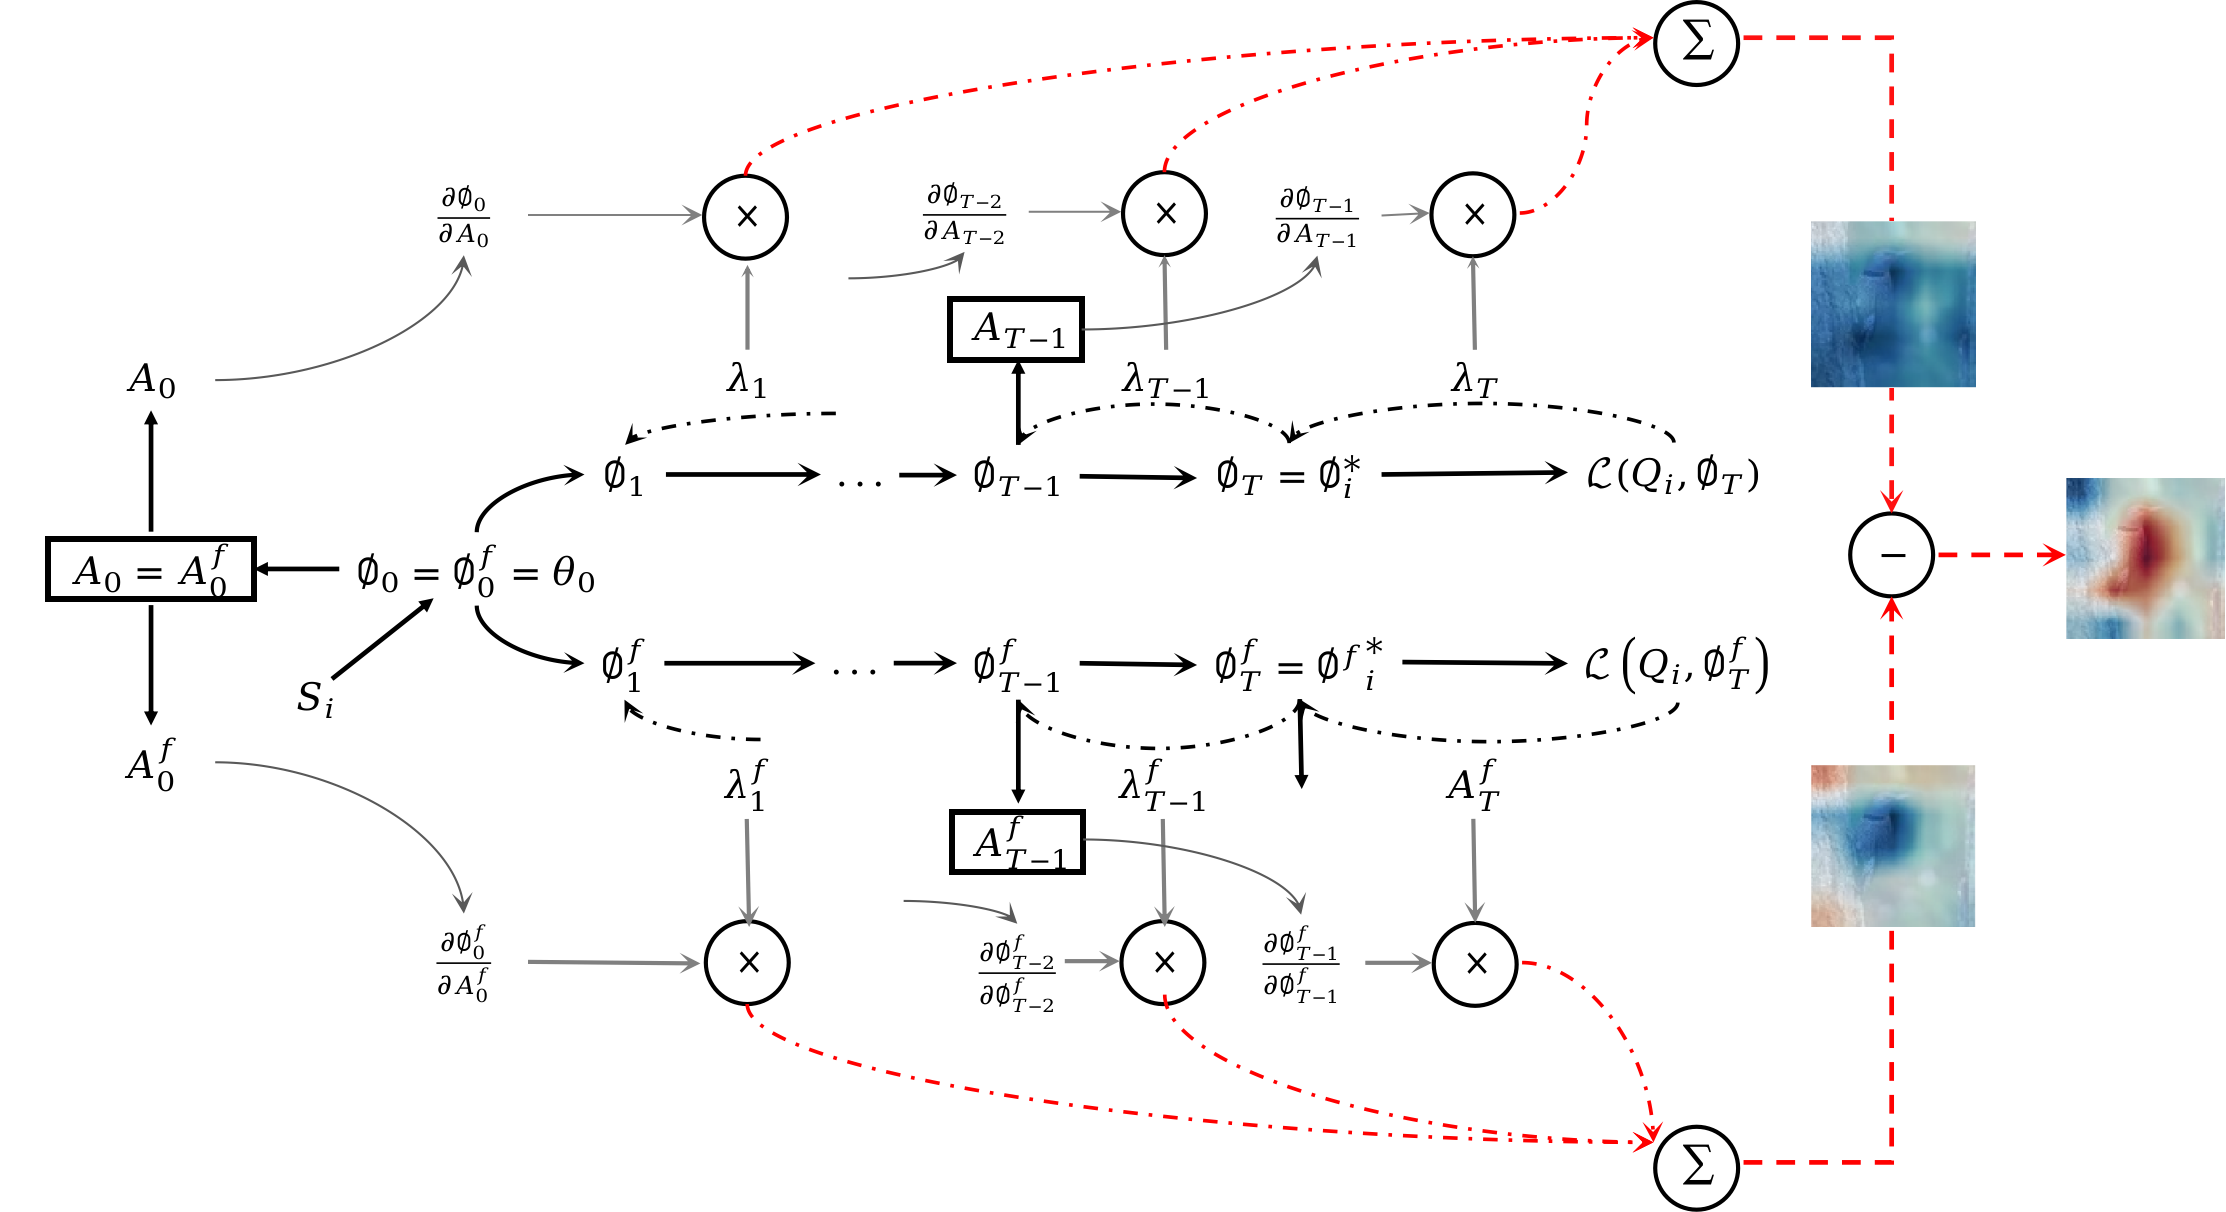
\includegraphics[width=0.9\textwidth]{../images/fama_pipeline.png}
    \caption{Pipeline tổng quan của \acrshort{fama}. Hai quỹ đạo (thích ứng toàn phần và can thiệp đóng băng) được sinh song song từ $S_i$; một lượt lan truyền ngược liên hợp duy nhất tính chuỗi $\{\lambda_t\}$ cho mỗi quỹ đạo; tại mỗi bước $t$, tín hiệu $\lambda_t$ được chiếu cục bộ lên bản đồ đặc trưng $A_{t-1}$; các bản đồ cục bộ được tích lũy theo $t$ rồi lấy hiệu giữa hai nhánh để ra bản đồ quy kết cuối cùng.}
    \label{fig:fama_pipeline}
\end{figure}

Để đảm bảo tính mạch lạc, phần còn lại của Mục~\ref{sec:fama} sẽ trình bày chi tiết theo trình tự bốn bước. (1) Khai triển đạo hàm quỹ đạo (Mục~\ref{subsec:derivative_expansion}). (2) Giải quyết chi phí tính toán bằng phương pháp liên hợp (Mục~\ref{subsec:adjoint}). (3) Định nghĩa đại lượng quy kết trên không gian đặc trưng (Mục~\ref{subsec:attribution_target}). và (4) Chiếu (projection) kết quả về không gian điểm ảnh (Mục~\ref{subsec:projection}).

\subsection{Khai triển đạo hàm qua quỹ đạo}
\label{subsec:derivative_expansion}
Xét một trong hai quỹ đạo (quá trình lập luận hoàn toàn tương tự đối với quỹ đạo còn lại). Gọi $g_{t-1} := \nabla_\phi \mathcal{L}(\phi_{(t-1)}, S_i)$ là gradient của hàm mất mát trên tập hỗ trợ. Theo quy tắc cập nhật vòng lặp trong (inner-loop) ở phương trình~\eqref{eq:inner_loop} cho $\phi_t = \phi_{t-1} - \alpha g_{t-1}$, ta thu được ma trận Jacobian cho một bước như sau.
\begin{equation}
    \frac{\partial \phi_t}{\partial \phi_{t-1}} = I - \alpha H_{t-1}, \qquad H_{t-1} := \nabla^2_\phi \mathcal{L}\big(\phi_{t-1}, S_i\big).
    \label{eq:step_jacobian}
\end{equation}

Theo đó, ta suy ra được vi phân trực tiếp qua thời gian (Backpropagation-Through-Time) bằng cách nhân dồn Jacobian từng bước qua toàn bộ $T$ bước cập nhật như sau.
\begin{equation}
    \frac{\partial \phi_T}{\partial \phi_0} = \prod_{t=1}^{T} \big(I - \alpha H_{t-1}\big),
    \label{eq:jacobian_product}
\end{equation}
Tích này tạo thành một ma trận có kích thước $P \times P$ (với $P$ là số lượng tham số trong mạng). Do đó, việc tính toán và lưu trữ tường minh ma trận này kéo theo chi phí bộ nhớ và thời gian lên đến $\mathcal{O}(TP^2)$, là một mức độ phức tạp hoàn toàn bất khả thi đối với các mạng nơ-ron học sâu.

Mặt khác, vì tập hỗ trợ $S_i$ đóng vai trò là đầu vào tường minh tại \emph{mọi} bước cập nhật. Nên theo quy tắc mắt xích (chain rule), đạo hàm của hàm mất mát đích $\mathcal{L}(Q_i, \phi_T)$ theo $S_i$ là tổng sự đóng góp của $S_i$ tại từng bước $t$.
\begin{equation}
    \frac{\partial \mathcal{L}(Q_i,\phi_{T})}{\partial S_i} \;=\; -\sum_{t=1}^{T} \alpha\, \lambda_t \cdot \frac{\partial^2 \mathcal{L}(\phi_{t-1}, S_i)}{\partial \phi_{t-1} \partial S_i},
    \label{eq:trajectory_expansion}
\end{equation}
trong đó $\lambda_t := \partial \mathcal{L}(Q_i,\phi_T)/\partial \phi_t$. (Được định nghĩa và chứng minh bằng quy nạp lùi tại Phụ lục~\ref{appendix:adjoint_proof}).

Mà từ cấu trúc phân rã ở phương trình~\eqref{eq:trajectory_expansion} này, có thể thấy được đạo hàm toàn cục của $\mathcal{L}(Q_i,\phi_T)$ hoàn toàn có thể chia tách thành $T$ số hạng cục bộ. Mà trong đó mỗi số hạng được đánh trọng số bởi $\lambda_t$. Dù vậy, bài toán tính $\lambda_t$ vẫn phải đối mặt với mức chi phí khổng lồ $\mathcal{O}(TP^2)$ nếu thực hiện khai triển Jacobian trực tiếp.

\subsection{Phương pháp liên hợp}
\label{subsec:adjoint}

Để vượt qua trở ngại về chi phí tính toán và bộ nhớ khi đánh giá ma trận Jacobian dọc theo quỹ đạo học, chúng tôi xây dựng cơ chế lan truyền dựa trên \emph{phương pháp trạng thái liên hợp} (Adjoint State Method). Nền tảng của phương pháp này xuất phát từ Nguyên lý cực đại Pontryagin trong lý thuyết điều khiển tối ưu.

Trong lý thuyết điều khiển liên tục, xét một hệ động lực với biến trạng thái $\mathbf{x}(t) = (x^1(t), \dots, x^n(t))$ và biến điều khiển $u(t)$ thay đổi theo hệ phương trình vi phân $\frac{dx^i}{dt} = f^i(\mathbf{x}(t), u(t))$. Để tính toán độ nhạy của một hàm mục tiêu tại thời điểm cuối $\Phi(\mathbf{x}(t_1))$ đối với sự thay đổi trạng thái ở một thời điểm $t$ bất kỳ, Pontryagin định nghĩa một vectơ liên hợp $\psi(t) = (\psi_1(t), \dots, \psi_n(t))$ tuân theo hệ phương trình liên hợp (adjoint system) ngược chiều thời gian:
\begin{equation}
    \frac{d\psi_i(t)}{dt} = - \sum_{\alpha=1}^n \frac{\partial f^\alpha(\mathbf{x}(t), u(t))}{\partial x^i} \psi_\alpha(t),
    \label{eq:pontryagin_continuous_component}
\end{equation}
hay được biểu diễn gọn dưới dạng ma trận Jacobian chuyển vị:
\begin{equation}
    \frac{d\psi(t)}{dt} = - \left( \frac{\partial f(\mathbf{x}(t), u(t))}{\partial \mathbf{x}} \right)^\top \psi(t),
    \label{eq:pontryagin_continuous}
\end{equation}
với điều kiện biên được khởi tạo tại điểm đích: $\psi(t_1) = \nabla_{\mathbf{x}} \Phi(\mathbf{x}(t_1))$. Hệ thức này cho phép lan truyền thông tin gradient từ tương lai về quá khứ mà không cần tính toán trực tiếp sự thay đổi tiến của toàn bộ quỹ đạo.

Trong ngữ cảnh của chúng tôi, quỹ đạo thời gian liên tục được rời rạc hóa thành các bước cập nhật tham số (gradient descent) $\phi_{t} = \phi_{t-1} - \alpha \nabla_{\phi} \mathcal{L}(\phi_{t-1})$. Lúc này, ma trận Jacobian của quá trình dịch chuyển đóng vai trò tương đương với toán tử tiến hóa $f$ của hệ thống, và vectơ liên hợp $\psi(t)$ của Pontryagin được chúng tôi ký hiệu và đối chiếu thành chuỗi biến rời rạc $\lambda_t$.

Quá trình tính toán chuỗi liên hợp $\{\lambda_t\}_{t=1}^T$ bắt đầu bằng việc khởi tạo điều kiện biên tại điểm cuối của quỹ đạo (tương đương $\psi(t_1)$):
\begin{equation}
    \lambda_T := \mathbb{E}_{Q_i \sim \mathcal{T}_i}\big[\nabla_\phi \mathcal{L}(Q_i, \phi_T)\big].
    \label{eq:adjoint_init}
\end{equation}
Đại lượng này được xấp xỉ bằng phương pháp Monte Carlo thông qua bootstrap phân tầng trên tập truy vấn $Q_i$. Từ mốc này, biến liên hợp $\lambda_t$ được lan truyền \emph{ngược} qua từng bước theo bản rời rạc hóa của phương trình~\eqref{eq:pontryagin_continuous}:
\begin{equation}
    \lambda_{t-1} = \lambda_t - \alpha\, H_{t-1}\, \lambda_t, \qquad t = T, T-1, \dots, 1.
    \label{eq:adjoint_recursion}
\end{equation}
trong đó $H_{t-1}$ là ma trận Hessian của hàm mất mát tại $\phi_{t-1}$.

\begin{proposition}[Tính tương đương của phép liên hợp]
\label{prop:adjoint_equivalence}
Với chuỗi $\lambda^{(t)}$ sinh ra bởi hệ phương trình~\eqref{eq:adjoint_init}--\eqref{eq:adjoint_recursion}, ta có đẳng thức thể hiện sự bảo toàn gradient: $\lambda^{(t)} = \partial \mathbb{E}_{Q_i}[\mathcal{L}(Q_i,\phi^{(T)})]/\partial \phi^{(t)}$ tại mọi bước $t = 0, 1, \dots, T$.
\end{proposition}

Từ mệnh đề~\ref{prop:adjoint_equivalence} ta hoàn toàn có thể thực hiện phép toán liên hợp nhằm tìm ra $\lambda_t$ tại mọi bước trong quỹ đạo mà không cần phải qua một chuỗi nhân Jacobian khổng lồ. Tuy nhiên, tính hợp lệ của phép tuyến tính hoá để đạt được hệ thức~\eqref{eq:adjoint_recursion} qua nhiều bước liên tiếp đòi hỏi các ràng buộc chặt chẽ về mặt không gian trạng thái sau.
 
\begin{assumption}[Tính trơn và ổn định của phép liên hợp]
\label{asm:adjoint_stability}
\leavevmode\newline\vspace{0.25em}
\begin{enumerate}[label=(\roman*)]
    \item $\mathcal{L}(\cdot, S_i)$ khả vi liên tục hai lần theo $\phi$ trong một lân cận mở chứa toàn bộ quỹ đạo $\{\phi_0, \dots, \phi_T\}$;
    \item Ma trận Hessian $H(\phi)$ thỏa mãn điều kiện liên tục Lipschitz, tức là tồn tại hằng số $L_H < \infty$ sao cho $\|H(\phi) - H(\phi')\| \le L_H \|\phi - \phi'\|$, đảm bảo sai số tuyến tính hoá tại mỗi bước bị chặn bởi $\mathcal{O}(\alpha^2)$;
    \item Tốc độ học $\alpha$ phải thỏa mãn bất đẳng thức $\alpha \le 2/\lambda_{\max}(H_{t-1})$ tại mọi bước $t$, nhằm đảm bảo toán tử $(I - \alpha H_{t-1})$ không giãn nở ($\|I - \alpha H_{t-1}\| \le 1$), từ đó ngăn hiện tượng chuỗi $\{\lambda_t\}$ bùng nổ qua $T$ bước lùi.
\end{enumerate}
\end{assumption}
Và với cơ chế thích ứng nhanh ($T\alpha \ll 1$), ta gần như hoàn toàn có thể thỏa mãn các ràng buộc này đối với các cấu trúc phổ trị riêng thông thường (chứng minh chi tiết tại Phụ lục~\ref{appendix:adjoint_proof}). 

Đồng thời khi chuyển sang hệ thức liên hợp~\eqref{eq:adjoint_recursion}, ta đã loại bỏ đi được rào cản về bộ nhớ bằng cách không cần phải lưu trữ và biểu diễn tường minh ma trận Hessian $H_{t-1}$ (vốn có kích thước rất lớn $P \times P$). Thay vào đó, quá trình này chỉ yêu tính trực tiếp \textbf{tích vô hướng Hessian-vector (HVP)}, $H_{t-1}\lambda_t$.

Để thực thi điều này, chúng tôi áp dụng kỹ thuật lan truyền ngược kép mà Pearlmutter đã đề xuất \cite{pearlmutter1994fast}. Đó là, thay vì tính ma trận Hessian $H$, ta hoàn toàn có thể tính đạo hàm có hướng (directional derivative) của gradient theo hướng của vector $\lambda_t$ như sau.
\begin{equation}
    H_{t-1}\lambda_t = \nabla_{\phi_{t-1}} \big\langle \nabla_{\phi_{t-1}} \mathcal{L}, \lambda_t \big\rangle
    \label{eq:hvp_trick}
\end{equation}
Tương đương với việc thực hiện hai lần lan truyền ngược (forward-over-reverse hoặc reverse-over-reverse) trong các triển khai thực tế. Với lần lan truyền đầu tiên tạo ra đồ thị tính toán cho tích vô hướng $\langle \nabla \mathcal{L}, \lambda_t \rangle$, và lần tiếp theo chính là lấy gradient của chính tích vô hướng đó.

Thông qua kỹ thuật HVP này, việc cập nhật $\lambda_{t-1}$ có thể được tính toán với chi phí không gian và thời gian tỷ lệ thuận với $\mathcal{O}(P)$. Kết quả là tổng chi phí qua $T$ bước được làm phẳng, giảm mạnh từ $\mathcal{O}(TP^2)$ xuống mức tuyến tính $\mathcal{O}(TP)$. Và chuỗi trọng số $\{\lambda^{(t)}\}$ thu được với chi phí thấp này sau đó sẽ đóng vai trò dẫn hướng cho việc quy kết trên không gian đặc trưng.

\subsection{Đại lượng quy kết}
\label{subsec:attribution_target}

Gọi $A_j := f_{\phi_j^{b}}(S_i) \in F$ trong đó $a_{jk}$ là biểu diễn đặc trưng của mẫu $x_k^S$ tại bước thứ $j$ của quỹ đạo (với kích thước $C \times H \times W$). Khác với các phương pháp giải thích tĩnh chỉ quan tâm đến một biểu diễn duy nhất ở cuối quỹ đạo $A_{T}$, \acrshort{fama} xử lý một \textbf{chuỗi biểu diễn} $\{A_0, \dots, A_{T-1}\}$, mỗi phần tử gắn với một trạng thái backbone khác nhau $\phi_j^{b}$ dọc theo quỹ đạo.

Do $A_j$ được tính toán lại từ đầu vào $S_i$ tại mỗi mốc thời gian thông qua một backbone $\phi_j^b$ không ngừng biến đổi, do đó không tồn tại một đại lượng $A$ toàn cục đóng vai trò trung gian cho toàn bộ quỹ đạo $T$ bước. Nói cách khác, thay vì có một phép biến đổi $S \to A \to \Delta M$ để có thể áp dụng quy tắc mắt xích một lần duy nhất, ta có $T$ phép biến đổi cục bộ tách biệt độc lập như sau. 
\begin{equation}
    S_i \xrightarrow{\ f_{\phi_{t-1}^{b}}\ } A_{t-1} \xrightarrow{\ } \mathcal{L}(\phi_{t-1}, S_i), \qquad t = 1, \dots, T,
    \label{eq:local_factorization}
\end{equation}

Nhận diện được cấu trúc này, \acrshort{fama} thực hiện cơ chế can thiệp cục bộ. Tại mỗi bước, bản đồ $A_{t-1}$ được ngắt khỏi mắt xích đạo hàm (stop-gradient), biến nó thành một biến lá (leaf variable) độc lập với toàn bộ lịch sử tính toán trước đó. Khi đó, đại lượng cần quy kết không còn là đạo hàm toàn cục, mà là một \textbf{họ} gồm $T$ giá trị phân bổ cục bộ.
\begin{equation}
    \mathrm{Attr}_{(t-1)} \;:=\; \frac{\partial}{\partial A_{(t-1)}}\Big[\lambda_t \cdot \nabla_{\phi} \mathcal{L}\big(\phi_{t-1}, S_i\big)\Big], \qquad t = 1,\dots,T,
    \label{eq:local_attr}
\end{equation}
Tại đây, $\lambda_t$ đóng vai trò trọng số tầm quan trọng, quy định mức độ ảnh hưởng của biến đổi tại bước $t$ lên hàm mất mát mục tiêu ở cuối quỹ đạo.
 
\subsection{Phép chiếu về không gian đầu vào và bản đồ quy kết}
\label{subsec:projection}

Khi $A_{t-1}$ đã bị cô lập thành biến độc lập $\tilde{A}_{t-1}$ thông qua thao tác ngắt đạo hàm ra khỏi mắt xích, hàm mất mát $\mathcal{L}(\phi_{t-1}, S_i)$ chỉ còn phụ thuộc tường minh vào phần đầu phân lớp (head) $\phi_{t-1}^h$ và biểu diễn $\tilde{A}_{t-1}$. Do phần thân mạng (backbone) đã bị đóng băng về mặt hình thức, đạo hàm của vô hướng $h_{t} := \lambda_t \cdot \nabla_\phi \mathcal{L}$ theo các tham số backbone sẽ triệt tiêu. Điều này ép buộc $\mathrm{Attr}_{t-1}$ phản ánh chính xác khối Hessian chéo $\partial^2 \mathcal{L}/\partial \phi_h \partial A$ — mang ý nghĩa quy kết trực tiếp đặc trưng đối với bộ phân lớp.

Từ tensor $\mathrm{Attr}_{t-1}$ (kích thước $C \times H \times W$), thuật toán tích hợp thành bản đồ nhiệt (CAM) theo công thức tiêu chuẩn của Grad-CAM \cite{selvaraju2020grad}, áp dụng riêng cho từng bước $t$:
\begin{align}
    w_t^c &= \frac{1}{HW}\sum_{i,j} \mathrm{Attr}_{t-1}^{(c,i,j)}, \label{eq:gap}\\
    \mathrm{CAM}_{t-1}^{(i,j)} &= \sum_{c} w_t^{c}\, A_{t-1}^{(c,i,j)}), \label{eq:cam_combine}\\
    \widehat{\mathrm{CAM}}_{t-1} &= \mathrm{Upsample}\big(\mathrm{CAM}_{t-1}, \label{eq:cam_upsample}
\end{align}
Trong đó, phương trình~\eqref{eq:gap} thực hiện gộp trung bình không gian theo kênh, phương trình~\eqref{eq:cam_combine} tính toán tổ hợp có trọng số, và \eqref{eq:cam_upsample} tiến hành nội suy song tuyến.

\textbf{Lưu ý về dấu:} Trái ngược với Grad-CAM vốn áp dụng hàm $\mathrm{ReLU}$ để loại bỏ tín hiệu âm, \acrshort{fama} \textbf{bảo toàn dấu} của $\widehat{\mathrm{CAM}}_{t-1}$. Bởi lẽ, cả vùng tạo ra chuyển giao tích cực (hướng $\Delta M$ theo chiều dương) và tiêu cực (chiều âm) đều là thông tin chẩn đoán quan trọngtrong ngữ cảnh phân tích độ lợi thích ứng.

Sau đó, các bản đồ cục bộ sẽ được tích lũy dọc theo từng bước để tạo thành bản đồ nhiệt cho một nhánh quỹ đạo hoàn chỉnh.
\begin{equation}
    \Phi(x_k^S) := \sum_{t=1}^{T} \alpha \, \widehat{\mathrm{CAM}}_{t-1}.
    \label{eq:branch_saliency}
\end{equation}

Quy trình này được thực thi độc lập cho cả hai nhánh quỹ đạo thích ứng toàn phần ($\Phi_{\text{full}}$) và quỹ đạo can thiệp đóng băng ($\Phi_{\text{freeze}}$). Do đó, bản đồ quy kết cuối cùng chính là kết quả của hiệu số giữa hai nhánh.

\begin{equation}
    \boxed{\Phi_{\text{FAMA}}(x_k^S) := \Phi_{\text{full}}(x_k^S) - \Phi_{\text{freeze}}(x_k^S).}
    \label{eq:fama_final_map}
\end{equation}

Về mặt ý nghĩa, vì nhánh $\Phi_{\text{freeze}}$ sử dụng biểu diễn tiền nghiệm tĩnh không đổi qua mọi bước, nó đóng vai trò là một \textbf{đường cơ sở tái sử dụng đặc trưng} (feature-reuse baseline). Do đó, phép trừ ở phương trình~\eqref{eq:fama_final_map} sẽ cô lập hoàn toàn phần đóng góp \emph{thuần túy} phát sinh do sự biến thiên của backbone dưới tác động của tập hỗ trợ. Việc này hoàn toàn đồng nhất với thành phần đóng góp cốt lõi $C_b$ đã được chứng minh trong Mệnh đề~\ref{prop:decomposition}.

Về mặt diễn giải, vùng $\Phi_{\text{FAMA}} > 0$ chỉ ra các đặc trưng mà khi được tinh chỉnh đã giúp giảm lỗi trên tập truy vấn (chuyển giao tích cực). Ngược lại, vùng $\Phi_{\text{FAMA}} < 0$ cảnh báo các đặc trưng gây hại (ví dụ: tương quan giả) khiến hiệu suất suy giảm khi thích ứng.

Tuy nhiên, vì phép nội suy ở phương trình~\eqref{eq:cam_upsample} dựa trên giả định rằng không gian (spatial correspondence) giữa lưới đặc trưng và ảnh gốc có tính tương thích. Do đó, \acrshort{fama} hoạt động hiệu quả trên các kiến trúc tích chập. Nhưng đối với các cấu trúc không bảo toàn không gian điểm ảnh (như các phương pháp dựa trên Transformer thuần túy), thuật toán sẽ cần có một số sự điều chỉnh tương ứng.

\section{Cơ sở đánh giá}
\label{sec:metrics}
Để đánh giá tính hiệu quả của một phương pháp diễn giải, ta không thể chỉ phụ thuộc vào tính trực quan hay thẩm mỹ của bản đồ quy kết, mà cần dựa trên hai tiêu chí học thuật cốt lõi. Thứ nhất, về \textbf{tính trung thực} (faithfulness), bản đồ quy kết phải phản ánh chính xác cơ chế hoạt động nội bộ của mô hình đang được diễn giải. Trong ngữ cảnh meta-learning, điều này đồng nghĩa với việc lời giải thích phải nắm bắt đúng quá trình thích ứng nhanh (fast adaptation) trên tập hỗ trợ $S_i$, thay vì chỉ biểu diễn một mối tương quan bề mặt giữa đầu vào và đầu ra. Thứ hai, về \textbf{tính đáng tin cậy} (trustworthiness): phương pháp diễn giải phải thực sự nhạy cảm với các yếu tố chi phối hệ thống. Cụ thể, trong bài toán này, kết quả quy kết bắt buộc phải phụ thuộc vào tri thức tiên nghiệm (prior knowledge) $\theta_0$ và nội dung ngữ nghĩa của $S_i$, chứ không phải là một phép biến đổi hình học cố định độc lập với những tri thức mô hình đã học được. Tiêu chí thứ hai này đòi hỏi phải được đánh giá thông qua các phép thử tính hợp lệ (sanity check), vốn đã được chứng minh là điều kiện \emph{cần} để một bản đồ quy kết có thể được tin cậy~\cite{adebayo2018sanity}.

 Nhằm điều chỉnh cho phù hợp với bối cảnh diễn giải trên quỹ đạo thích ứng đã trình bày ở Mục~\ref{sec:fama}, nơi đối tượng phân tích không phải là một kết quả dự đoán tĩnh mà là một đại lượng động ($\Delta M$) được tổng hợp qua nhiều trạng thái tham số trung gian. Chúng tôi đưa ra ba bài kiểm chứng lần lượt đánh giá tính trung thực và tính hợp lệ, được trình bày chi tiết như sau.
 
\subsection{Bài kiểm chứng dựa trên xóa và đo hai chiều (\acrfull{biadt})}
\label{subsec:biadt}
Nguyên tắc chung của một bài kiểm tra xóa và đo (deletion test) là nếu bản đồ quy kết thực sự định vị đúng vùng chi phối đầu ra của mô hình, thì việc tuần tự che đi các vùng được đánh giá là quan trọng nhất (theo thứ tự giảm dần) sẽ làm đầu ra thay đổi nhanh hơn đáng kể so với việc xóa theo thứ tự ngẫu nhiên. Tuy nhiên, khác với các bài kiểm tra xóa-và-đo truyền thống thường chỉ đánh giá sự suy giảm theo một chiều duy nhất của độ tin cậy của dự đoán, thì đại lượng $\Phi_{\text{FAMA}}$ chứa \emph{dấu} nhằm đại diện cho chiều hướng ảnh hưởng. Cụ thể, các vùng có $\Phi_{\text{FAMA}}>0$ được cho là nguồn gốc của chuyển giao tích cực, ngược lại, những vùng có $\Phi_{\text{FAMA}}<0$ thì ứng với nguồn gốc của việc chuyển giao tiêu cực (Mục~\ref{subsec:projection}). Chính vì đặc thù này, quy trình kiểm định tính trung thực đối với $\Phi_{\text{FAMA}}$ cần được thiết kế theo \textbf{hai chiều} độc lập, với mỗi chiều kiểm chứng đúng một nửa giả thuyết về dấu.
 
\textbf{Thiết lập.} Với mỗi mẫu hỗ trợ $x_k^S \in S_i$, thông qua thuật toán phân đoạn chuẩn (ví dụ như SLIC~\cite{achanta2012slic}) không gian điểm ảnh của $x_k^S$ được phân thành $P$ vùng ảnh (superpixel) rời rạc $\{s_1, \dots, s_P\}$ và được gán bằng một điểm số quy kết tổng hợp.
\[
    \bar{\Phi}(s_p) := \frac{1}{|s_p|}\sum_{(i,j)\in s_p} \Phi_{\text{FAMA}}(x_k^S)_{i,j},
\]
và sắp xếp toàn bộ $P$ vùng theo thứ tự \emph{tăng dần} của $\bar\Phi$ (từ vùng có đóng góp tiêu cực nhất đến vùng có đóng góp tích cực nhất). Với một tỉ lệ xóa $\rho \in [0,1]$, gọi $S_i^{(\rho,\pi)}$ là tập hỗ trợ nhận được sau khi làm mờ/thay bằng giá trị nền $\lfloor \rho P \rfloor$ vùng ảnh đầu tiên theo thứ tự xóa $\pi$, với $\pi$ nhận một trong ba giá trị:
\begin{itemize}
    \item $\pi = \texttt{tăng dần}$: xóa lần lượt từ đầu danh sách đã sắp xếp — tức xóa các vùng có $\Phi_{\text{FAMA}}$ \emph{âm nhất} trước;
    \item $\pi = \texttt{giảm dần}$: xóa theo chiều ngược lại — tức xóa các vùng có $\Phi_{\text{FAMA}}$ \emph{dương nhất} trước;
    \item $\pi = \texttt{ngẫu nhiên}$: xóa theo một hoán vị ngẫu nhiên của $P$ vùng, lấy trung bình trên nhiều lần lặp độc lập để làm đường cơ sở kiểm soát (control baseline).
\end{itemize}
Với mỗi tổ hợp $(\rho,\pi)$, ta thay $S_i$ bằng $S_i^{(\rho,\pi)}$, ta thực hiện việc tính độ lợi thích ứng (adaptation gain) theo phương trình~\eqref{eq:adaptation_gain}, ký hiệu $\Delta M(\rho,\pi)$.
 
\textbf{Giả thuyết kiểm định.} Nếu $\Phi_{\text{FAMA}}$ là một bản đồ quy kết trung thực, ta kỳ vọng hai chiều xóa-và-đo mang lại hai xu hướng đối lập, và cùng tách biệt rõ rệt khỏi đường cơ sở ngẫu nhiên:
\begin{itemize}
    \item Theo chiều \texttt{giảm dần} (xóa vùng dương nhất trước): vì các vùng bị loại bỏ sớm chính là nguồn gốc của chuyển giao tích cực, $\Delta M(\rho,\allowbreak\texttt{giảm dần})$ phải suy giảm nhanh hơn đáng kể so với $\Delta M(\rho,\allowbreak\texttt{ngẫu nhiên})$ khi $\rho$ tăng.
    \item Theo chiều \texttt{tăng dần} (xóa vùng âm nhất trước): vì các vùng bị loại bỏ sớm chính là nguồn gốc của chuyển giao tiêu cực, việc loại bỏ chúng đồng nghĩa với "làm sạch" $S_i$, nên $\Delta M(\rho,\allowbreak\texttt{tăng dần})$ phải tăng nhanh hơn đáng kể so với $\Delta M(\rho,\allowbreak\texttt{ngẫu nhiên})$ khi $\rho$ tăng.
\end{itemize}
Hai xu hướng này được lượng hóa bằng diện tích lệch khỏi đường ngẫu nhiên, tương tự chỉ số AOPC (Area Over Perturbation Curve) trong các bài kiểm tra xóa cổ điển:
\begin{equation}
    \begin{split}
    \mathrm{ABC}_{\downarrow} := \int_0^1 \Big[\Delta M(\rho,\texttt{ngẫu nhiên}) - \Delta M(\rho,\texttt{giảm dần})\Big]\,d\rho, \\
    \mathrm{ABC}_{\uparrow} := \int_0^1 \Big[\Delta M(\rho,\texttt{tăng dần}) - \Delta M(\rho,\texttt{ngẫu nhiên})\Big]\,d\rho.
    \end{split}
    \label{eq:abc_metric}
\end{equation}
Và một bản đồ quy kết được xem là vượt qua \acrshort{biadt} nếu cả $\mathrm{ABC}_{\downarrow}$ lẫn $\mathrm{ABC}_{\uparrow}$ đều dương và có ý nghĩa thống kê trên nhiều tác vụ lấy mẫu. Việc đòi hỏi \emph{cả hai} chiều đồng thời đạt ý nghĩa thống kê thay vì chỉ một chiều như các bài kiểm tra xóa-và-đo thông thường chính là điểm khác biệt cốt lõi giúp \acrshort{biadt} kiểm chứng trực tiếp giả thuyết giữ nguyên dấu của $\Phi_{\text{FAMA}}$ (Mục~\ref{subsec:projection}).
 
\subsection{Bài kiểm chứng độ tỉnh táo thông qua việc phá hủy tri thức tiên nghiệm $\theta_0$}
\label{subsec:sanity_theta0}
 
Bài kiểm tra ở Mục~\ref{subsec:biadt} xác nhận rằng $\Phi_{\text{FAMA}}$ có quan hệ nhân quả với $\Delta M$ thông qua can thiệp trực tiếp lên $S_i$. Tuy nhiên, nó không loại trừ khả năng bản đồ quy kết chỉ đơn thuần phản ánh cấu trúc hình học chung của kiến trúc mạng (ví dụ hoạt động tương tự một bộ dò biên cố định), mà hoàn toàn không phụ thuộc vào \emph{nội dung} của tri thức tiên nghiệm $\theta_0$ đã học được qua giai đoạn meta-training. Đây chính là hiện tượng đã được chỉ ra ở bài kiểm tra ngẫu nhiên hóa tham số mô hình (model parameter randomization test), \textit{nhiều phương pháp giải thích phổ biến cho ra bản đồ gần như không đổi ngay cả khi toàn bộ trọng số mô hình bị thay bằng giá trị ngẫu nhiên}~\cite{adebayo2018sanity}.
 
\textbf{Thiết lập.} Gọi $\theta_0^{b} = \{W_1, \dots, W_L\}$ là $L$ lớp tham số phần thân trích xuất của mô hình. Với mỗi $\ell = 1, \dots, L$, ta có được một phiên bản tri thức tiên nghiệm bị phá hủy theo tầng (cascading randomization) là $\theta_0^{b,(\ell)}$, trong đó $\ell$ lớp cuối cùng $\{W_{L-\ell+1}, \dots, W_L\}$ — tính từ lớp gần đầu ra ngược về lớp gần đầu vào — được khởi tạo lại ngẫu nhiên theo đúng phân phối khởi tạo gốc của kiến trúc, còn $L-\ell$ lớp còn lại giữ nguyên giá trị có được ở giai đoạn meta-training. Với $\ell = L$, toàn bộ backbone bị phá hủy hoàn toàn. Việc phá hủy theo tầng thay vì phá hủy toàn bộ một lượt cho phép xác định \emph{lớp nào} là nơi bản đồ quy kết bắt đầu phân kỳ, và đặc biệt phù hợp với FAMA vì đối tượng quy kết của nó là một chuỗi biểu diễn $\{A_j\}$ (Mục~\ref{subsec:attribution_target}) vốn được trích xuất trực tiếp từ chính các lớp này.
 
Với mỗi $\theta_0^{b,(\ell)}$, ta thực hiện áp dụng toàn bộ quy trình thích ứng nhanh và phép chiếu \acrshort{fama} (Mục~\ref{sec:fama}) từ đầu, thay $\theta_0^b$ gốc bằng $\theta_0^{b,(\ell)}$, thu được bản đồ quy kết bị nhiễu $\Phi_{\text{FAMA}}^{(\ell)}$. Sau đó ta so sánh $\Phi_{\text{FAMA}}^{(\ell)}$ với bản đồ gốc $\Phi_{\text{FAMA}}$ (ứng với $\ell = 0$, không can thiệp) bằng hệ số tương quan hạng Spearman hoặc Pearson $\rho_s\big(\Phi_{\text{FAMA}}^{(\ell)}, \Phi_{\text{FAMA}}\big)$, tính trên toàn bộ điểm ảnh của $x_k^S$.
 
\textbf{Giả thuyết kiểm định.} Nếu $\Phi_{\text{FAMA}}$ thực sự phản ánh tri thức tiên nghiệm đã học ở $\theta_0^b$, hệ số $\rho_s\big(\Phi_{\text{FAMA}}^{(\ell)}, \Phi_{\text{FAMA}}\big)$ phải suy giảm đơn điệu và có ý nghĩa thống kê khi $\ell$ tăng, tiệm cận về mức tương quan giữa hai bản đồ độc lập ngẫu nhiên (ước lượng bằng cách hoán vị ngẫu nhiên $\Phi_{\text{FAMA}}$) tại $\ell = L$. Ngược lại, nếu $\rho_s$ vẫn giữ mức cao bất kể $\ell$, điều đó đồng nghĩa \acrshort{fama} thất bại phép kiểm tra tỉnh táo này. Bản đồ quy kết khi đó chỉ là một hàm số của kiến trúc mạng và nội dung ảnh đầu vào, hoàn toàn tách rời khỏi những gì mô hình đã thực sự học được từ meta-training, và do đó không thể được diễn giải như một lời giải thích có ý nghĩa cho hành vi thích ứng của mô hình.
 
\subsection{Bài kiểm chứng độ tỉnh táo thông qua việc can thiệp vào tập hỗ trợ $S_i$}
\label{subsec:sanity_support}
 
Song song với việc kiểm tra độ nhạy đối với $\theta_0$, ta cần kiểm tra độ nhạy của $\Phi_{\text{FAMA}}$ đối với chính nội dung ngữ nghĩa của tập hỗ trợ $S_i$, là nguyên nhân quyết định trực tiếp quỹ đạo thích ứng. Đây là phiên bản mở rộng của bài kiểm tra ngẫu nhiên hóa dữ liệu/nhãn (data/label randomization test)~\cite{adebayo2018sanity} sang bối cảnh few-shot, được thiết kế để bao quát ba dạng phổ biến của hiện tượng tác vụ không đồng nhất (heterogeneous task)~\cite{si2025meta} gồm nhãn nhiễu (label noise), tác vụ khó (task difficulty), và tác vụ nằm ngoài phân phối so với phân phối gốc (out-of-distribution). Với mỗi dạng, chúng tôi định nghĩa một phép can thiệp $S_i \to S_i'$ tương ứng.
 
\textbf{(a) Hoán vị nhãn (label permutation).} Áp dụng một hoán vị ngẫu nhiên $\sigma$ lên tập $N$ lớp của tác vụ $\mathcal{T}_i$, và gán lại $y_k^S \gets \sigma(y_k^S)$ cho mọi mẫu hỗ trợ trong khi vẫn giữ nguyên $x_k^S$. Việc này phá vỡ hoàn toàn mối liên kết ngữ nghĩa giữa ảnh và nhãn mà quá trình thích ứng nhanh dựa vào.
 
\textbf{(b) Tăng độ khó tác vụ (hard-task perturbation).} Làm mờ (Gaussian blur) hoặc thêm nhiễu lên $x_k^S$, sao cho ranh giới phân biệt giữa các lớp trong $\mathcal{T}_i$ trở nên mờ nhạt hơn nhằm mục đích mô phỏng một tác vụ khó, nơi tín hiệu phân biệt hữu ích cho backbone khai thác bị suy giảm.
 
\textbf{(c) Trộn tác vụ ngoài phân phối (OOD task mixing).} Thay toàn bộ các mẫu trong tập hỗ trợ $S_i$ bằng các mẫu lấy từ một tác vụ $\mathcal{T}_j$ khác tách biệt so với $\mathcal{T}_i$, nhưng vẫn giữ nguyên tập truy vấn $Q_i$ (ví dụ một tập dữ liệu khác hoặc một tập hợp lớp không liên quan), tạo ra một tác vụ lai không đồng nhất mà quá trình meta-training chưa từng chuẩn bị.
 
Với mỗi phép can thiệp, ta thực hiện áp dụng quy trình thích ứng và \acrshort{fama} trên $S_i'$ để thu được $\Phi_{\text{FAMA}}'$ và $\Delta M'$, sau đó so sánh với $\Phi_{\text{FAMA}}$ và $\Delta M$ gốc.
 
\textbf{Giả thuyết kiểm định.} Cả ba phép can thiệp trên đều được thiết kế để phá hoại cấu trúc hữu ích của $S_i$ theo những cách khác nhau, nên đều được kỳ vọng đẩy quá trình thích ứng nhanh về phía chuyển giao tiêu cực nhiều hơn. Tức là $\Delta M'$ có xu hướng thấp hơn $\Delta M$ một cách có ý nghĩa thống kê. Tương ứng, một bản đồ quy kết trung thực phải phản ánh đúng sự dịch chuyển này, phân bố không gian của $\Phi_{\text{FAMA}}'$ phải lệch về phía âm nhiều hơn so với $\Phi_{\text{FAMA}}$. Ngược lại, nếu $\Phi_{\text{FAMA}}'$ không có sự khác biệt có ý nghĩa thống kê so với $\Phi_{\text{FAMA}}$ dù $S_i$ đã bị can thiệp nghiêm trọng đến mức làm suy giảm rõ rệt $\Delta M'$, điều đó đồng nghĩa bản đồ quy kết đã tách rời khỏi nội dung ngữ nghĩa thực sự của $S_i$, và do đó không đáng tin cậy.
 
Ngoài ra, việc thực hiện cả ba bài kiểm chứng trên cần được lặp lại trên một tập hợp lớn các tác vụ $\mathcal{T}_i$ được lấy mẫu ngẫu nhiên tại thời điểm meta-testing, thay vì chỉ minh họa trên một vài tác vụ đơn lẻ. Do đó, các chỉ số tổng hợp ($\mathrm{ABC}_\downarrow$, $\mathrm{ABC}_\uparrow$, hệ số tương quan $\rho_s$, và độ lệch phân phối của $\Phi_{\text{FAMA}}'$) vì vậy được báo cáo dưới dạng phân phối qua nhiều tác vụ, kèm khoảng tin cậy và kiểm định ý nghĩa thống kê so với đường cơ sở tương ứng, thay vì một con số đơn lẻ dễ gây hiểu lầm. Toàn bộ kết quả thực nghiệm của ba bài kiểm chứng này, cùng các phân tích định tính bổ sung trên một số tác vụ minh họa, sẽ được trình bày chi tiết ở Chương~\ref{Chapter4}.


\chapter{Kết quả thực nghiệm}
\label{Chapter4}

Chương này trình bày các thực nghiệm được thực hiện nhằm đánh giá độ tin cậy (\textit{faithfulness}) và tính đúng đắn (\textit{sanity}) của bản đồ độ nổi bật (\textit{saliency map}) sinh ra bởi mô hình giải thích (\textit{explainer}) trong bối cảnh meta-learning. Ba nhóm thực nghiệm được tiến hành, tương ứng với ba mục tiêu đánh giá khác nhau:

\begin{itemize}
    \item \textbf{Đánh giá độ tin cậy hai chiều (Bi-directional Faithfulness – biADT):} kiểm tra xem vùng ảnh mà saliency map cho là quan trọng có thực sự ảnh hưởng đến khả năng thích nghi (\textit{adaptation}) của mô hình hay không.
    \item \textbf{Kiểm tra sanity bằng ngẫu nhiên hóa tham số mô hình (Model Parameter Randomization):} kiểm tra xem saliency map có thực sự phụ thuộc vào tham số đã học của mạng hay không, tránh trường hợp giải thích chỉ là một bộ dò biên (\textit{edge detector}) không liên quan đến mô hình.
    \item \textbf{Kiểm tra sanity với support set dựa trên tính không đồng nhất của tác vụ (HetroM):} kiểm tra độ nhạy của saliency map trước các biến động của tập hỗ trợ (\textit{support set}) — nhãn nhiễu, ảnh khó (mờ), và mẫu ngoài phân phối (OOD) — nhằm phản ánh tính chất không đồng nhất giữa các tác vụ vốn là đặc trưng của HetroM.
\end{itemize}

Tất cả các thực nghiệm được thực hiện trên tập kiểm tra (\textit{test set}) với mô hình đã huấn luyện, sử dụng số bước thích nghi $T = T_{test}$.

\section{Đánh giá độ tin cậy hai chiều (Bi-directional Faithfulness – biADT)}

\subsection{Mục tiêu}
Mục tiêu của thực nghiệm này là kiểm chứng tính faithfulness của saliency map: liệu các vùng ảnh được gán độ quan trọng dương và độ quan trọng âm có thực sự phản ánh đúng vai trò của chúng đối với quá trình thích nghi (\textit{inner-loop adaptation}) của mô hình hay không.

\subsection{Phương pháp}
Với mỗi tác vụ, quy trình đánh giá bao gồm:
\begin{enumerate}
    \item \textbf{Phân hạng theo siêu điểm ảnh:} Ảnh hỗ trợ được phân đoạn bằng SLIC. Các siêu điểm ảnh được xếp hạng theo ba chế độ:
    \begin{itemize}
        \item \textit{pos}: Loại bỏ dần vùng có độ nổi bật dương cao nhất.
        \item \textit{neg}: Loại bỏ dần vùng có độ nổi bật âm thấp nhất.
        \item \textit{random}: Loại bỏ ngẫu nhiên (baseline).
    \end{itemize}
    \item \textbf{Xóa dần thông tin ảnh:} Thay thế vùng ảnh bằng ảnh nền đã làm mờ Gaussian.
    \item \textbf{Đo độ lợi thích nghi:} Tính diện tích dưới đường cong (AUC) cho từng chế độ: $AUC_{pos}, AUC_{neg}, AUC_{random}$.
    \item \textbf{Tính chỉ số:}
    \begin{itemize}
        \item $PDA = AUC_{random} - AUC_{pos}$
        \item $NDA = AUC_{neg} - AUC_{random}$
        \item $Combined = PDA + NDA$
    \end{itemize}
\end{enumerate}

\subsection{Kết quả}
\begin{table}[h]
\centering
\caption{Kết quả đánh giá độ tin cậy hai chiều (biADT)}
\begin{tabular}{|l|c|}
\hline
\textbf{Chỉ số} & \textbf{Giá trị trung bình} \\ \hline
PDA (Positive Deletion Advantage) & 0.1861 \\ \hline
NDA (Negative Deletion Advantage) & 0.2892 \\ \hline
\textbf{Combined (PDA + NDA)} & \textbf{0.4752} \\ \hline
\end{tabular}
\end{table}

\subsection{Nhận xét}
Kết quả cho thấy cả PDA và NDA đều dương, khẳng định saliency map có ý nghĩa nhân quả thực sự. NDA lớn hơn PDA cho thấy mô hình rất nhạy trong việc xác định các vùng "gây nhiễu" (\textit{distractor}).

\section{Kiểm tra sanity bằng ngẫu nhiên hóa tham số mô hình}

\subsection{Phương pháp}
Các tham số của mạng được khởi tạo lại ngẫu nhiên theo từng lớp (cascading) từ lớp cuối về lớp đầu. Saliency map mới được so sánh với saliency map gốc bằng hệ số tương quan Pearson và Spearman.

\subsection{Kết quả}
\begin{table}[h]
\centering
\caption{Kết quả kiểm tra sanity theo ngẫu nhiên hóa tham số}
\begin{tabular}{|c|c|c|c|}
\hline
\textbf{Thứ tự} & \textbf{Lớp bị phá hủy} & \textbf{Pearson} & \textbf{Spearman} \\ \hline
0 & Lớp cuối (gần đầu ra) & 0.0871 & 0.0846 \\ \hline
1-7 & Các lớp trung gian & $\approx 0$ & $\approx 0$ \\ \hline
8 & Lớp đầu (gần đầu vào) & -0.0050 & -0.0064 \\ \hline
\end{tabular}
\end{table}

\subsection{Nhận xét}
Hệ số tương quan xấp xỉ 0 cho thấy saliency map phụ thuộc mạnh mẽ vào các tham số đã học của toàn bộ mạng, vượt qua phép kiểm tra sanity kinh điển.

\section{Kiểm tra sanity với support set dựa trên tính không đồng nhất của tác vụ}

\subsection{Kịch bản thực nghiệm}
\begin{itemize}
    \item \textbf{Noisy check:} Hoán vị nhãn (flip ratio = 0.8).
    \item \textbf{Hard check:} Làm mờ ảnh bằng bộ lọc Gaussian ($\sigma = 3.0$).
    \item \textbf{OOD check:} Trộn 2 lớp từ tác vụ khác vào support set.
\end{itemize}

\subsection{Kết quả}
\begin{table}[h]
\centering
\caption{Kết quả kiểm tra sanity với support set nhiễu loạn}
\begin{tabular}{|l|c|c|}
\hline
\textbf{Kịch bản} & \textbf{Pearson} & \textbf{Spearman} \\ \hline
Noisy & 0.2578 & 0.2499 \\ \hline
Hard & 0.2664 & 0.2576 \\ \hline
OOD & 0.3398 & 0.3305 \\ \hline
\end{tabular}
\end{table}

\subsection{Nhận xét}
Saliency map có sự thay đổi hợp lý trước các biến động của dữ liệu, không bị "trơ" nhưng vẫn giữ được tính cấu trúc không gian nhất định.

\section{Tổng kết}
Các thực nghiệm khẳng định phương pháp giải thích đề xuất vừa đảm bảo tính tin cậy nhân quả (faithfulness), vừa đạt chuẩn về tính đúng đắn (sanity) và phản ánh tốt đặc trưng không đồng nhất của dữ liệu trong HetroM.
%\section{Trích dẫn tài liệu}

%Dùng lệnh $\textbackslash cite$ để trích dẫn một hoặc nhiều tài liệu tham khảo.
%Tài liệu tham khảo có thể là trang web~\cite{Listings,HDLVThS}, bài báo khoa học~\cite{1994-Cavnar}, sách~\cite{1984-TeX-Knuth,2006-DDien,2006-NPTV}, bài tạp chí~\cite{1989-TED} hoặc các nguồn tham khảo khác. 
%Lưu ý khi trích dẫn tài liệu tham khảo, cần viết câu sao cho bỏ phần trong cặp ngoặc vuông đi thì câu vẫn đầy đủ ý nghĩa.
%Ví dụ, thay vì viết ``Nghiên cứu~\cite{1989-TED} chỉ ra rằng ... '' thì nên viết ``Nghiên cứu của Zhang~\cite{1989-TED} chỉ ra rằng ...''.
%Một ví dụ khác, thay vì viết ``... như trong công trình nghiên cứu~\cite{1994-Cavnar}.'' thì nên viết ``... như trong công trình nghiên cứu của Cavnar và Trenkle~\cite{1994-Cavnar}.''

%\section{Chèn mã nguồn}

%Để chèn mã nguồn, cần dùng package listings~\cite{Listings}:

%\begin{lstlisting}
%\usepackage{listings}
%\end{lstlisting}

%Mã nguồn có thể được chèn trực tiếp như sau:

%\begin{lstlisting}[language=Python]
%print "Hello, World!"
%\end{lstlisting}

%hoặc chèn thông qua tập tin chứa mã nguồn trong thư mục $SourceCode$ như sau:

%\lstinputlisting[language=C++]{SourceCode/hello.cpp}

%Để chèn mã giả, cần dùng package algorithm~\cite{Algorithm}:

%\begin{lstlisting}
%\usepackage{algorithm}
%\end{lstlisting}

%Có thể chèn mã giả vào như sau:

%\begin{algorithm}
%\caption{My algorithm}\label{euclid}
%\begin{algorithmic}[1]
%\Procedure{MyProcedure}{}
%\State $\textit{stringlen} \gets \text{length of }\textit{string}$
%\State $i \gets \textit{patlen}$
%\BState \emph{top}:
%\If {$i > \textit{stringlen}$} \Return false
%\EndIf
%\State $j \gets \textit{patlen}$
%\BState \emph{loop}:
%\If {$\textit{string}(i) = \textit{path}(j)$}
%\State $j \gets j-1$.
%\State $i \gets i-1$.
%\State \textbf{goto} \emph{loop}.
%\State \textbf{close};
%\EndIf
%\State $i \gets i+\max(\textit{delta}_1(\textit{string}(i)),\textit{delta}_2(j))$.
%\State \textbf{goto} \emph{top}.
%\EndProcedure
%\end{algorithmic}
%\end{algorithm}

%\section{Hình ảnh}

%Để chèn hình ảnh, cần dùng package graphicx~\cite{Figures}:

%\begin{lstlisting}
%\usepackage{graphicx}
%\end{lstlisting}

%Hình \ref{fig:vd1}, hình \ref{fig:vd2} là một số ví dụ về chèn hình ảnh.

%\begin{figure}[htp]
%\centering
%
\includegraphics[width=6 cm]{images/logo-khtn.png}
%\caption{Hình ví dụ 1}
%\label{fig:vd1}
%\end{figure}

%\begin{figure*}[htp]
%\centering
%
\includegraphics[width=40 mm]{images/logo-khtn.png}
%\caption{Hình ví dụ 2}
%\label{fig:vd2}
%\end{figure*}

%\section{Bảng biểu}

%Để tạo bảng biểu, tham khảo thêm tại sharelatex.com~\cite{Tables}.
%Bảng~\ref{tab:vd1} là một ví dụ về bảng.
%Ngoài ra, có một số tool online~\footnote{Như trang http://www.tablesgenerator.com/} có thể được dùng để tạo bảng biểu một cách trực quan.

%\begin{table}[ht]
%\caption{Bảng ví dụ 1}

%\label{tab:vd1}%
%\begin{center}
%\begin{tabular}{ |p{3cm}||p{3cm}|p{3cm}|p{3cm}|  }
 %\hline
 %\multicolumn{4}{|c|}{Country List} \\
 %\hline
 %Country Name     or Area Name& ISO ALPHA 2 Code &ISO ALPHA 3 Code&ISO numeric Code\\
 %\hline
 %Afghanistan   & AF    &AFG&   004\\
 %Aland Islands&   AX  & ALA   &248\\
 %Albania &AL & ALB&  008\\
 %Algeria    &DZ & DZA&  012\\
 %American Samoa&   AS  & ASM&016\\
 %Andorra& AD  & AND   &020\\
 %Angola& AO  & AGO&024\\
 %\hline
%\end{tabular}
%\end{center}
%\end{table}

%\section{Công thức}

%Công thức có thể chèn vào trong cùng một dòng như $ \sqrt{a^2+b^2} $ hoặc nằm trên dòng riêng như công thức~\ref{eu_eqn}.

%\begin{equation} \label{eu_eqn}
%x = a_0 + \frac{1}{a_1 + \frac{1}{a_2 + \frac{1}{a_3 + a_4}}}
%\end{equation}

\chapter{Kết luận}
\label{Chapter5}
Nhằm giải quyết các câu hỏi nghiên cứu về hiện tượng chuyển giao tiêu cực (negative transfer) trong quá trình thích ứng nhanh của \acrfull{maml} đã được phân tích tại Mục~\ref{sec:research_urgency}, luận văn đã đề xuất thành công phương pháp hậu diễn giải (post-hoc explaination) dựa trên độ lợi thích ứng $\Delta M$ và phương pháp \acrfull{fama}.

Cụ thể, thông qua đại lượng $\Delta M$, chiều hướng tác động (có lợi hoặc có hại) của việc thích ứng nhanh hoàn toàn có thể được xác định một cách tường minh. Mà dựa trên kết quả đó, \acrshort{fama} thông qua việc phân bổ liên hợp trong không gian đặc trưng chung $F$ mà định vị chính xác các vùng không gian trên tập hỗ trợ $S_i$ là nguyên nhân gốc rễ gây ra tác động này xuyên suốt toàn bộ quỹ đạo thích ứng qua nhiều bước, nhờ đó mà có thể trực quan hóa được hiện tượng "thiên lệch ngữ cảnh" (contextual bias) dẫn đến hiện tượng chuyển giao tiêu cực.

Đồng thời, các thực nghiệm kiểm chứng cũng đã khẳng định phương pháp mà chúng tôi đề ra hoàn toàn trung thực và đáng tin cậy với việc chỉ ra cơ chế thích ứng nhanh. Các kết quả từ việc thực hiện \acrfull{biadt} đạt mức ý nghĩa thống kê cao ($p<0.001$) ở cả hai chiều tích cực lẫn tiêu cực. Và, hai bài kiểm tra tính tỉnh táo (sanity checks) qua can thiệp tri thức tiên nghiệm $\theta_0$ và dữ liệu $S_i$ đã chứng minh bản đồ quy kết của \acrshort{fama} thực sự bắt nguồn từ tri thức đã học và nội dung dữ liệu của tập hỗ trợ, điều này đồng nghĩa với việc triệt tiêu hoàn toàn sự chi phối của các yếu tố cấu trúc mạng trơ. Nhờ đó, luận văn mang đến một công cụ diễn giải hoàn toàn mới, khả vi và độc lập với dữ liệu meta-training cho lĩnh vực meta-learning.

\section{Hạn chế và hướng phát triển}

Tuy nhiên, nghiên cứu hiện tại vẫn còn một số hạn chế do việc sử dụng kiến trúc nông. Việc thực nghiệm trên kiến trúc Conv4 khiến lưới đặc trưng ở khối tích chập cuối có độ phân giải không gian thô, gây ra hiện tượng "tràn màu" (spatial bleeding) khi định vị các vật thể nhỏ và tạo ra mức sai số biên khá lớn trong đánh giá \acrshort{biadt}. Ngoài ra, kiến trúc nông cũng khiến kịch bản can thiệp OOD chưa phản ánh đúng độ nhạy kỳ vọng do sự tương đồng về thống kê thị giác cấp thấp giữa các tập dữ liệu, và thang đo phá hủy mạng ($\ell=0,\dots,4$) chưa đủ mịn để quan sát chi tiết sự sụt giảm hiệu năng.

Từ những hạn chế trên, luận văn đề xuất 4 hướng phát triển tiềm năng trong tương lai:
\begin{enumerate}
    \item \textbf{Cải thiện độ phân giải không gian:} Mở rộng thực nghiệm sang các kiến trúc backbone sâu hơn (như ResNet-12) nhằm giải quyết triệt để hiện tượng tràn màu.
    \item \textbf{Tinh chỉnh kịch bản can thiệp:} Sử dụng các tập dữ liệu phi-vật-thể (như Places hoặc ảnh kết cấu) làm nhiễu OOD để tạo ra phép thử Sanity Check khắc nghiệt và chính xác hơn.
    \item \textbf{Kiểm chứng tính phổ quát:} Khái quát hóa khung đánh giá $\Delta M$ và \acrshort{fama} sang các biến thể tối ưu hóa khác (ANIL, BOIL, Meta-SGD) trong số các phương pháp thuộc họ \acrshort{maml} (\acrshort{maml}-based).
    \item \textbf{Can thiệp chủ động:} Kết hợp \acrshort{fama} với các cơ chế can thiệp biểu diễn (như HSFM) nhằm tiến xa hơn từ việc chẩn đoán sang việc tự động hiệu chỉnh tập hỗ trợ $S_i$, khép kín vòng lặp giữa diễn giải XAI và cải thiện trực tiếp hiệu năng mô hình.
\end{enumerate}


% Công trình của tác giả (nếu không có thì comment 02 dòng dưới)
%\addcontentsline{toc}{chapter}{Danh mục công trình của tác giả}
%\include{Appendix/publish}

% In tài liệu tham khảo
\addcontentsline{toc}{chapter}{Tài liệu tham khảo}
\printbibheading[title={Tài liệu tham khảo}]

\printbibliography[heading=subbibliography, title={Tiếng Việt}, keyword=Viet, resetnumbers=true]

\DeclareNameAlias{sortname}{family-given}
\DeclareNameAlias{default}{family-given}

\printbibliography[heading=subbibliography, title={Tiếng Anh}, notkeyword=Viet, resetnumbers=true]
% ===================================================================== %
% CHÚ Ý: phải gán lại resetnumbers=số tài liệu tham khảo tiếng Việt + 1 %
% ===================================================================== %

% Phần phụ lục
% Chứng minh các mệnh đề
\appendix

\chapter{Chứng minh Mệnh đề~\ref{prop:decomposition}}
\label{appendix:taylor_proof}

Chương này chứng minh chi tiết Mệnh đề~\ref{prop:decomposition} (Mục~\ref{sec:definition_AG}): dưới chế độ thích ứng nhanh (Giả thuyết~\ref{asm:fast_adaptation}), $\Delta M = -C_b + O\big((T\alpha)^2\big)$.

\section{Thiết lập và khai triển bậc hai}

Ký hiệu $\theta_0 = (\theta_0^b, \theta_0^h)$. Xét hàm mất mát kỳ vọng trên tập truy vấn $L(\phi) := \mathbb{E}_{Q_i\sim\mathcal{T}_i}[\mathcal{L}(Q_i,\phi)]$, giả sử khả vi liên tục hai lần trong một lân cận mở chứa $\theta_0$ và toàn bộ quỹ đạo. Đặt $_b := \nabla_b L(\theta_0)$, $g_h := \nabla_h L(\theta_0)$, $H_{bb} := \nabla^2_{bb} L(\theta_0)$, $H_{bh} := \nabla^2_{bh} L(\theta_0)$, $H_{hh} := \nabla^2_{hh} L(\theta_0)$.

Gọi $\Delta b_T := \phi_T^b - \theta_0^b$, $\Delta h_T := \phi_T^h - \theta_0^h$ (nhánh thích ứng toàn phần) và $\Delta h_T^f := \phi_T^{f,h} - \theta_0^h$ (nhánh can thiệp). Vì backbone bị đóng băng ở nhánh can thiệp, $\Delta b_T^f = 0$.

Khai triển Taylor bậc hai của $L$ quanh $\theta_0$ cho mỗi nhánh:
\begin{align}
    L(\phi_T) &= L(\theta_0) + g_b^\top \Delta b_T + g_h^\top \Delta h_T \nonumber\\
    &\quad + \tfrac{1}{2}\Delta b_T^\top H_{bb} \Delta b_T + \Delta b_T^\top H_{bh} \Delta h_T + \tfrac{1}{2}\Delta h_T^\top H_{hh} \Delta h_T + o(\|\Delta\|^2), \label{eq:taylor_full}\\[4pt]
    L(\phi_T^f) &= L(\theta_0) + g_h^\top \Delta h_T^f + \tfrac{1}{2}{\Delta h_T^f}^\top H_{hh} \Delta h_T^f + o(\|\Delta h_T^f\|^2). \label{eq:taylor_frozen}
\end{align}
Trừ~\eqref{eq:taylor_frozen} cho~\eqref{eq:taylor_full} và dùng định nghĩa $\Delta M = L(\phi_T^f) - L(\phi_T)$ (Phương trình~\eqref{eq:adaptation_gain}, đã lấy kỳ vọng theo $Q_i$), số hạng $L(\theta_0)$ triệt tiêu và ta thu được chính xác Phương trình~\eqref{eq:decomposition}:
\begin{equation}
    \begin{split}
        \Delta M = & -\,\underbrace{\Big[g_b^\top \Delta b_T + \tfrac{1}{2}\Delta b_T^\top H_{bb} \Delta b_T + \Delta b_T^\top H_{bh} \Delta h_T\Big]}_{C_b} \\
    &+ \underbrace{\Big[g_h^\top(\Delta h_T^f - \Delta h_T) + \tfrac{1}{2}\big({\Delta h_T^f}^\top H_{hh} \Delta h_T^f - \Delta h_T^\top H_{hh} \Delta h_T\big)\Big]}_{R_h},
    \end{split}
    \label{eq:decomposition}
\end{equation}

\section{Bậc độ lớn của các số hạng dịch chuyển}

\begin{lemma}[Dịch chuyển tích lũy $O(T\alpha)$]
\label{lem:displacement_order}
Giả sử $\|\nabla_\phi \mathcal{L}(\phi,S_i)\| \le G$ trong lân cận quỹ đạo. Khi đó $\|\Delta b_T\|, \|\Delta h_T\|, \|\Delta h_T^f\| = O(T\alpha)$.
\end{lemma}
\begin{proof}
Mỗi bước cập nhật inner-loop~\eqref{eq:inner_loop} dịch chuyển tham số một lượng $\alpha\|\nabla_\phi\mathcal{L}\| \le \alpha G$. Sau $T$ bước, theo bất đẳng thức tam giác, tổng dịch chuyển tích lũy bị chặn bởi $T\alpha G = O(T\alpha)$, áp dụng như nhau cho cả ba đại lượng vì cả hai nhánh đều thực hiện đúng $T$ bước cập nhật dạng này (nhánh can thiệp chỉ khác ở việc phần backbone bị ghi đè về $\theta_0^b$ sau mỗi bước, không ảnh hưởng đến bậc của phần head).
\end{proof}

\begin{lemma}[Độ lệch giữa hai quỹ đạo head là $O((T\alpha)^2)$]
\label{lem:head_divergence}
Đặt $\delta_j := \Delta h_j - \Delta h_j^f$. Dưới điều kiện $\nabla_h\mathcal{L}(\cdot,S_i)$ Lipschitz với hằng số $L$ theo $\phi$ (hệ quả của Giả thuyết~\ref{asm:adjoint_stability}(ii)), ta có $\delta_T = O\big((T\alpha)^2\big)$. Đặc biệt, tại $T=1$, $\delta_1 = 0$ \textbf{tuyệt đối}.
\end{lemma}
\begin{proof}
Tại $j=1$: cả hai nhánh cùng xuất phát từ $\phi_0 = \phi_0^f = \theta_0$, nên bước gradient đầu tiên của head trùng nhau tuyệt đối, $\delta_1 = 0$.

Với $j \ge 2$, từ quy tắc cập nhật:
\[
    \delta_j = \delta_{j-1} - \alpha\Big[\nabla_h\mathcal{L}(\phi_{j-1},S_i) - \nabla_h\mathcal{L}(\phi_{j-1}^f,S_i)\Big].
\]
Hai đối số $\phi_{j-1} = (\phi_{j-1}^b,\phi_{j-1}^h)$ và $\phi_{j-1}^f=(\theta_0^b,\phi_{j-1}^{f,h})$ khác nhau ở backbone một lượng $\Delta b_{j-1} = O((j-1)\alpha)$ (Bổ đề~\ref{lem:displacement_order}) và ở head một lượng $\delta_{j-1}$. Do tính Lipschitz,
\begin{align*}
    \big\|\nabla_h\mathcal{L}(\phi_{j-1},S_i) - \nabla_h\mathcal{L}(\phi_{j-1}^f,S_i)\big\| &\le L\big(\|\Delta b_{j-1}\| + \|\delta_{j-1}\|\big)\\
                                                                                            &= O\big((j-1)\alpha + \|\delta_{j-1}\|\big).
\end{align*}
Suy ra
\[
    \|\delta_j\| \le (1+\alpha L)\|\delta_{j-1}\| + O\big((j-1)\alpha^2\big).
\]
Với $\delta_1=0$ và khai triển đệ quy, do $T\alpha\ll1$ (Giả thuyết~\ref{asm:fast_adaptation}) nên $(1+\alpha L)^{T} = 1+O(T\alpha)$ vẫn bị chặn:
\begin{align*}
    \|\delta_T\| &\le \sum_{k=1}^{T-1} O(k\alpha^2)\cdot\big(1+O(\alpha)\big)^{T-1-k}\\
    &= O(\alpha^2)\sum_{k=1}^{T-1} k \cdot\big(1+O(T\alpha)\big)\\
    &= O(\alpha^2 T^2) = O\big((T\alpha)^2\big).
\end{align*}
\end{proof}

\section{Bậc độ lớn của $C_b$ và $R_h$, và kết luận}

Từ Bổ đề~\ref{lem:displacement_order}: số hạng tuyến tính $g_b^\top\Delta b_T = O(T\alpha)$ là bậc chủ đạo trong $C_b$; hai số hạng bậc hai còn lại của $C_b$ đều là $O((T\alpha)^2)$. Vậy $C_b = O(T\alpha)$.

Từ Bổ đề~\ref{lem:head_divergence}: số hạng tuyến tính của $R_h$ là $g_h^\top(\Delta h_T^f - \Delta h_T) = -g_h^\top\delta_T = O\big((T\alpha)^2\big)$; các số hạng bậc hai còn lại của $R_h$ (hiệu hai dạng toàn phương) cũng có bậc $O\big((T\alpha)^2\big)$ vì $\delta_T$ là bậc chủ đạo của hiệu $\Delta h_T^f$ và $\Delta h_T$. Vậy $R_h = O\big((T\alpha)^2\big)$, và
\[
    \Delta M = -C_b + R_h = -C_b + O\big((T\alpha)^2\big),
\]
đúng như Phương trình~\eqref{eq:leading_order}, hoàn tất chứng minh Mệnh đề~\ref{prop:decomposition}. $\blacksquare$

Đặc biệt, với $T=1$, Bổ đề~\ref{lem:head_divergence} cho $\delta_1=0$ tuyệt đối, kéo theo $R_h=0$ \emph{chính xác} (không chỉ là vô cùng bé), khớp với nhận xét tại Mục~\ref{sec:definition_AG}.

\chapter{Chứng minh phương pháp liên hợp và cận sai số}
\label{appendix:adjoint_proof}

Chương này chứng minh Mệnh đề~\ref{prop:adjoint_equivalence} (tính tương đương của $\lambda^{(t)}$), suy ra công thức khai triển~\eqref{eq:trajectory_expansion}, và thiết lập cận ổn định/sai số dưới Giả thuyết~\ref{asm:adjoint_stability}.

\section{Tính tương đương của biến liên hợp (chứng minh Mệnh đề~\ref{prop:adjoint_equivalence})}

Xét một nhánh quỹ đạo bất kỳ (lập luận đối xứng cho nhánh còn lại), viết gọn $\bar{L}(\phi) := \mathbb{E}_{Q_i}[\mathcal{L}(Q_i,\phi)]$. Ta chứng minh bằng quy nạp lùi rằng
\[
    \lambda^{(t)} = \frac{\partial \bar{L}(\phi^{(T)})}{\partial \phi^{(t)}}, \qquad t = T, T-1, \dots, 0.
\]

\textbf{Cơ sở quy nạp ($t=T$).} Vì $\phi^{(T)}$ là đối số trực tiếp của $\bar{L}$, ta có:
\[
    \partial\bar{L}(\phi^{(T)})/\partial\phi^{(T)} = \nabla_\phi\bar{L}(\phi^{(T)}) = \lambda^{(T)}
\]
theo đúng định nghĩa~\eqref{eq:adjoint_init}.

\textbf{Bước quy nạp.} Giả sử mệnh đề đúng tại $t$, ta chứng minh đúng tại $t-1$. Vì $\phi^{(T)}$ phụ thuộc vào $\phi^{(t-1)}$ duy nhất thông qua trung gian $\phi^{(t)}$ (quy tắc cập nhật~\eqref{eq:inner_loop} là một chuỗi Markov tham số), quy tắc dây chuyền cho
\[
    \frac{\partial \bar L(\phi^{(T)})}{\partial \phi^{(t-1)}} = \left(\frac{\partial \phi^{(t)}}{\partial \phi^{(t-1)}}\right)^{\!\top} \frac{\partial \bar L(\phi^{(T)})}{\partial \phi^{(t)}} \overset{\text{gt quy nạp}}{=} \big(I-\alpha H_{t-1}\big)^{\top}\lambda^{(t)},
\]
sử dụng Jacobian một bước đã tính ở Phương trình~\eqref{eq:step_jacobian}. Vì $H_{t-1} = \nabla^2_\phi\mathcal{L}(\phi^{(t-1)},S_i)$ là ma trận Hessian, nó đối xứng ($H_{t-1}^\top = H_{t-1}$), nên
\[
    \big(I-\alpha H_{t-1}\big)^{\top}\lambda^{(t)} = \lambda^{(t)} - \alpha H_{t-1}\lambda^{(t)} = \lambda^{(t-1)}
\]
đúng theo định nghĩa đệ quy~\eqref{eq:adjoint_recursion}. Vậy $\partial\bar L(\phi^{(T)})/\partial\phi^{(t-1)} = \lambda^{(t-1)}$, hoàn tất bước quy nạp. $\blacksquare$

\textbf{Nhận xét quan trọng.} Chứng minh trên không dùng bất kỳ phép xấp xỉ nào — Jacobian~\eqref{eq:step_jacobian} là \emph{chính xác} (đạo hàm của một bước gradient descent), nên với $H_{t-1}$ được tính đúng (không xấp xỉ), đệ quy liên hợp~\eqref{eq:adjoint_recursion} tính $\lambda^{(t)}$ một cách \emph{chính xác tuyệt đối}, không phải xấp xỉ bậc nhất. Đây là điểm khác biệt căn bản so với các phương pháp liên hợp cho hệ động lực liên tục (neural ODE) vốn phải rời rạc hóa một phương trình vi phân — ở đây hệ đã rời rạc sẵn (inner-loop là SGD hữu hạn bước), nên không phát sinh sai số rời rạc hóa.

\section{Suy ra công thức khai triển~\eqref{eq:trajectory_expansion}}

Xem $\phi^{(t)} = \Psi_t(\phi^{(t-1)}, S_i) := \phi^{(t-1)} - \alpha\nabla_\phi\mathcal{L}(\phi^{(t-1)},S_i)$ là một hệ động lực rời rạc trong đó $S_i$ xuất hiện lặp lại như một \emph{tham số dùng chung} tại mọi bước $t=1,\dots,T$. Theo quy tắc đạo hàm tổng (total derivative) cho tham số dùng chung qua nhiều bước của một chuỗi hàm hợp,
\begin{align*}
    \frac{d\bar L(\phi^{(T)})}{dS_i} &= \sum_{t=1}^{T} \left(\frac{\partial \Psi_t}{\partial S_i}\Big|_{\phi^{(t-1)}}\right)^{\!\top} \left(\frac{\partial \phi^{(T)}}{\partial \phi^{(t)}}\right)^{\!\top} \nabla_\phi \bar L(\phi^{(T)}) \\
    &= \sum_{t=1}^{T} \left(\frac{\partial \Psi_t}{\partial S_i}\Big|_{\phi^{(t-1)}}\right)^{\!\top} \lambda^{(t)},
\end{align*}
Trong đó bước cuối dùng đúng kết quả vừa chứng minh ở trên vì 
\[
(\partial\phi^{(T)}/\partial\phi^{(t)})^\top\nabla_\phi\bar L(\phi^{(T)}) = \partial\bar L(\phi^{(T)})/\partial\phi^{(t)} = \lambda^{(t)}
\]

Mà $\Psi_t(\phi^{(t-1)},S_i) = \phi^{(t-1)} - \alpha\nabla_\phi\mathcal{L}(\phi^{(t-1)},S_i)$,
\[
    \frac{\partial \Psi_t}{\partial S_i}\Big|_{\phi^{(t-1)}} = -\alpha\,\frac{\partial^2 \mathcal{L}(\phi^{(t-1)},S_i)}{\partial \phi^{(t-1)}\partial S_i}.
\]
Thay vào, ta thu được chính xác Phương trình~\eqref{eq:trajectory_expansion}:
\[
    \frac{\partial \bar L(\phi^{(T)})}{\partial S_i} = -\sum_{t=1}^{T}\alpha\,\lambda^{(t)}\cdot\frac{\partial^2\mathcal{L}(\phi^{(t-1)},S_i)}{\partial\phi^{(t-1)}\partial S_i}.
\]
Áp dụng công thức này riêng biệt cho nhánh thích ứng toàn phần ($\phi^{(T)}=\phi_T$) và nhánh can thiệp ($\phi^{(T)}=\phi_T^f$), rồi lấy hiệu theo đúng định nghĩa $\Delta M$ ở Phương trình~\eqref{eq:adaptation_gain}, ta thu được công thức $\partial\Delta M/\partial S_i$ dùng làm điểm xuất phát của Mục~\ref{sec:fama}. $\blacksquare$

\section{Ổn định của đệ quy liên hợp (chứng minh dựa trên Giả thuyết~\ref{asm:adjoint_stability})}

\begin{proposition}[Không giãn nở]
\label{prop:nonexpansive}
Dưới Giả thuyết~\ref{asm:adjoint_stability}(iii), $\|\lambda^{(t-1)}\| \le \|\lambda^{(t)}\|$ với mọi $t$, do đó $\|\lambda^{(0)}\| \le \|\lambda^{(T)}\|$: chuỗi $\{\lambda^{(t)}\}$ không bùng nổ qua $T$ bước lùi.
\end{proposition}
\begin{proof}
Vì $H_{t-1}$ đối xứng, nó chéo hóa trực giao được với các trị riêng thực $\{\mu_i\}$. Theo (iii), $\alpha \le 2/\lambda_{\max}(H_{t-1})$, nên với mọi trị riêng $\mu_i \in [\lambda_{\min}, \lambda_{\max}]$ của $H_{t-1}$, giá trị riêng tương ứng $1-\alpha\mu_i$ của toán tử $I-\alpha H_{t-1}$ thỏa $|1-\alpha\mu_i|\le 1$ (vì $0\le\alpha\mu_i\le\alpha\lambda_{\max}\le2$, nên $1-\alpha\mu_i\in[-1,1]$). Do đó $\|I-\alpha H_{t-1}\|_{\text{op}} \le 1$, và từ~\eqref{eq:adjoint_recursion}: $\|\lambda^{(t-1)}\| = \|(I-\alpha H_{t-1})\lambda^{(t)}\| \le \|\lambda^{(t)}\|$.
\end{proof}

\begin{proposition}[Cận sai số khi $H_{t-1}$ được ước lượng xấp xỉ]
\label{prop:error_propagation}
Trong triển khai thực tế, $\lambda^{(T)}$ ở Phương trình~\eqref{eq:adjoint_init} và các tích Hessian–vector $H_{t-1}\lambda^{(t)}$ đều được ước lượng bằng bootstrap phân tầng hữu hạn trên $Q_i$ (Mục~\ref{subsec:adjoint}), do đó chịu sai số thống kê. Giả sử tại mỗi bước $t$, sai số ước lượng của tích Hessian–vector bị chặn bởi $\|\widehat{H_{t-1}\lambda^{(t)}} - H_{t-1}\lambda^{(t)}\| \le \varepsilon$. Khi đó, dưới Giả thuyết~\ref{asm:adjoint_stability}(ii)–(iii), sai số tích lũy sau $T$ bước lùi bị chặn bởi
\[
    \big\|\hat\lambda^{(0)} - \lambda^{(0)}\big\| \le T\alpha\varepsilon.
\]
\end{proposition}
\begin{proof}
Đặt $e_t := \hat\lambda^{(t)} - \lambda^{(t)}$ là sai số tích lũy tại bước $t$ (với $e_T=0$ nếu bỏ qua sai số ước lượng $\lambda^{(T)}$ ban đầu, hoặc cộng thêm nếu có). Từ đệ quy xấp xỉ $\hat\lambda^{(t-1)} = \hat\lambda^{(t)} - \alpha\widehat{H_{t-1}\lambda^{(t)}}$ và đệ quy đúng~\eqref{eq:adjoint_recursion},
\[
    e_{t-1} = \big(I-\alpha H_{t-1}\big)e_t - \alpha\big(\widehat{H_{t-1}\lambda^{(t)}} - H_{t-1}\lambda^{(t)}\big).
\]
Lấy chuẩn hai vế, dùng $\|I-\alpha H_{t-1}\|_{\text{op}}\le1$ (Mệnh đề~\ref{prop:nonexpansive}) và giả thiết sai số từng bước $\le\varepsilon$:
\[
    \|e_{t-1}\| \le \|e_t\| + \alpha\varepsilon.
\]
Khai triển đệ quy từ $t=T$ (với $e_T=0$) xuống $t=0$ qua $T$ bước, mỗi bước cộng thêm tối đa $\alpha\varepsilon$:
\[
    \|e_0\| \le T\alpha\varepsilon.
\]
\end{proof}

\textbf{Ý nghĩa thực nghiệm.} Mệnh đề~\ref{prop:error_propagation} cho thấy sai số của toàn bộ bản đồ quy kết $\Phi_{\text{FAMA}}$ do việc xấp xỉ Monte Carlo trên $Q_i$ (thay vì lấy kỳ vọng chính xác) tăng \emph{tuyến tính} theo $T\alpha$ — đúng bậc mà chế độ thích ứng nhanh (Giả thuyết~\ref{asm:fast_adaptation}, $T\alpha\ll1$) giữ ở mức nhỏ. Đây là căn cứ lý thuyết cho việc chọn số lượng bootstrap $\texttt{num\_bootstraps}$ đủ lớn (nhằm giảm $\varepsilon$) trong cài đặt tại Mục~\ref{subsec:adjoint}, thay vì phải tăng theo cấp số nhân với $T$.


\end{document} 
